%% DOC: http://mirror.ctan.org/macros/latex/contrib/koma-script/scrguide.pdf
\documentclass[
	% DEFAULT: final, a4paper, 11pt
	twoside,
	DIV11,				% Seitengroesse (siehe scrguide.pdf)
	BCOR5mm,			% Zusaetzlicher Rand auf der Innenseite
	pagesize,			% Schreibt die Papiergroesse in die Datei, wichtig fuer Konvertierungen
	headsepline,		% Linie unter Kopfzeile
	parskip=half,		% Abstand zwischen zwei Abs�tzen
	bibtotoc,			% Bibliographie ins Inhaltsverzeichnis
	liststotoc,			% Abb.- und Tabellenverzeichnis ins Inhaltsverzeichnis
	cleardoubleempty	% Vakatseiten bleiben leer (etwa Seite vor einem Kapitel, das auf rechts beginnt)
]{scrbook}

%% Preambel
\usepackage[bottom=4cm, right=4cm]{geometry}

%~~~~~~~~~~~~~~~~~~~~~~~~~~~~~~
%% LOAD FIRST
%~~~~~~~~~~~~~~~~~~~~~~~~~~~~~~

%% Encoding
\usepackage[latin1]{inputenc}

%% Sprache
%  ftp://tug.ctan.org/pub/tex-archive/macros/latex/required/babel/babel.pdf
\usepackage[english]{babel}
\usepackage{blindtext}
%% Besserer Flattersatz (Linksbuendig, statt Blocksatz)
%  ftp://tug.ctan.org/pub/tex-archive/macros/latex/contrib/ms/ragged2e.pdf
\usepackage{ragged2e}

%% Bilder
%  ftp://tug.ctan.org/pub/tex-archive/macros/latex/required/graphics/grfguide.pdf
\usepackage[]{graphicx}

%% Farben
%  ftp://tug.ctan.org/pub/tex-archive/macros/latex/contrib/xcolor/xcolor.pdf
% Incompatible: Do not load when using pstricks !
\usepackage[table,usenames,dvipsnames]{xcolor} % Load for using rowcolors command in tables


%\usepackage[nointegrals]{wasysym}

%% Mathematik Basispaket
%  ftp://tug.ctan.org/pub/tex-archive/macros/latex/required/amslatex/math/amsldoc.pdf
\usepackage[]{amsmath}



% damit es nicht zu "no room for new \dimen"-Fehler kommt
\usepackage{etex}

\usepackage{tikz}
\usepackage{tkz-graph}
%  \usepackage{ifthen}
%  \usepackage{xstring}
%  \usepackage{calc}
%  \usepackage{pgfopts}

% See http://pgfplots.sourceforge.net/pgfplots.pdf
\usepackage{pgfplots}
\usepackage{pgfplotstable}
\usetikzlibrary{pgfplots.groupplots}
\usetikzlibrary{patterns}

% argument #1: any options
\newenvironment{customlegend}[1][]{%
    \begingroup
    % inits/clears the lists (which might be populated from previous
    % axes):
    \csname pgfplots@init@cleared@structures\endcsname
    \pgfplotsset{#1}%
}{%
    % draws the legend:
    \csname pgfplots@createlegend\endcsname
    \endgroup
}%

% makes \addlegendimage available (typically only available within an
% axis environment):
\def\addlegendimage{\csname pgfplots@addlegendimage\endcsname}

\usepackage{epstopdf}


%prevent number and text in list of figures to overlap
\makeatletter
\renewcommand*\l@figure{\@dottedtocline{1}{1.5em}{3em}}% 3em instead of 2.3em
\let\l@table\l@figure
\makeatother


%~~~~~~~~~~~~~~~~~~~~~~~~~~~~~~
%% TEXT
%~~~~~~~~~~~~~~~~~~~~~~~~~~~~~~

%% Schriftart

%% http://www.tug.dk/FontCatalogue/mathfonts.html



\usepackage{lmodern}
%\usepackage{kpfonts}
%\usepackage{mathptmx}
%\usepackage[sc]{mathpazo}
%\usepackage{charter}

\usepackage[T1]{fontenc}
%\usepackage{ae,aecompl}

%Optischer Randausgleich mit pdfTeX
\usepackage[%
	expansion=false, % if true: better typography, but larger PDF file (and not compatible with all fonts)
	protrusion=true
]{microtype}

%% Zum Unterstreichen
%  ftp://tug.ctan.org/pub/tex-archive/macros/latex/contrib/misc/ulem.sty
\usepackage[normalem]{ulem}

%%% Doc: ftp://tug.ctan.org/pub/tex-archive/macros/latex/contrib/soul/soul.pdf
\usepackage{soul}	% Unterstreichen, Sperren

%% Control the look & feel of the captions from floating environments like figure and table.
%  ftp://tug.ctan.org/pub/tex-archive/macros/latex/contrib/caption/caption.pdf
\usepackage{caption}
% Aussehen der Captions
\captionsetup{
   margin = 10pt,
   font = {small,rm},
   labelfont = {small,bf},
   format = plain, % oder 'hang'
   indention = 0em,  % Einruecken der Beschriftung
   labelsep = colon, %period, space, quad, newline
   justification = RaggedRight, % justified, centering
   singlelinecheck = true, % false (true=bei einer Zeile immer zentrieren)
   position = bottom %top
}
%%% Bugfix Workaround (Matthias Pospiech!?)
\DeclareCaptionOption{parskip}[]{}
\DeclareCaptionOption{parindent}[]{}

%% �berschriften komlett Umdefinieren
%  ftp://tug.ctan.org/pub/tex-archive/macros/latex/contrib/titlesec/titlesec.pdf
\usepackage{titlesec}

%% Mehrere Text-Spalten
\usepackage{multicol}

%%
% Doc: ftp://tug.ctan.org/pub/tex-archive/macros/latex/contrib/paralist/paralist.pdf
\usepackage{paralist}

%% Better than 'paralist' and 'enumerate' because it uses a keyvalue interface !
%  Do not load together with package 'enumerate'.
%  ftp://tug.ctan.org/pub/tex-archive/macros/latex/contrib/enumitem/enumitem.pdf
\usepackage{enumitem}

%% Schriftanpassung nach scrguide.pdf
\setkomafont{subsection}{\sffamily}

%% Chapter-Style definieren
% --> Rechtsb�ndig: Gro�e Kapitelnummer, darunter der Name
\titleformat{\chapter}[display]
{\filleft\usekomafont{chapter}\Huge}
{\fontsize{100pt}{50pt}\selectfont\thechapter}
{-2ex} %is vertical space in [display] mode
%Platz vor dem ganzen Krempel
{\vspace{1ex}} %1ex ist die H�he von x im aktuellen Font
%Platz danach
[\vspace{1ex}]


\usepackage{nowidow}


%~~~~~~~~~~~~~~~~~~~~~~~~~~~~~~
%% TABELLEN (tabularx wird von ltxtable geladen!?)
%~~~~~~~~~~~~~~~~~~~~~~~~~~~~~~

%% Tabellen ueber mehere Seiten
%  ftp://tug.ctan.org/pub/tex-archive/macros/latex/contrib/carlisle/ltxtable.pdf
\usepackage{ltxtable} % Longtable + tabularx
                      % (multi-page tables) + (auto-sized columns in a fixed width table)
%% bessere Abstaende innerhalb der Tabelle (Layout))
%  ftp://tug.ctan.org/pub/tex-archive/macros/latex/contrib/booktabs/booktabs.pdf
\usepackage{booktabs}

%% Erweiterte Funktionen innerhalb von Tabellen
%  ftp://tug.ctan.org/pub/tex-archive/macros/latex/contrib/multirow/multirow.sty
\usepackage{multirow} % Mehrfachspalten

%% Tabellen: Ausrichtung an Komma oder Punkt
\usepackage{dcolumn}

\usepackage{pbox}
\usepackage{footnote}

%~~~~~~~~~~~~~~~~~~~~~~~~~~~~~~
%% FARBEN
%~~~~~~~~~~~~~~~~~~~~~~~~~~~~~~

\definecolor{sectioncolor}{RGB}{0, 0, 0}    % Schwarz

% Farbe des Textes
\definecolor{textcolor}{RGB}{0, 0, 0}        % Schwarz

% Farbe fuer grau hinterlegte Boxen (fuer Paket framed.sty)
\definecolor{shadecolor}{gray}{0.90}

% Farben fuer die Links im PDF
\definecolor{pdfurlcolor}{rgb}{0.6,0,0}
\definecolor{pdffilecolor}{rgb}{0,0.4,0}
\definecolor{pdflinkcolor}{rgb}{0,0,0.75}

% Java Syntax Highlighting
\definecolor{javared}{rgb}{0.6,0,0} % for strings
\definecolor{javagreen}{rgb}{0.25,0.5,0.35} % comments
\definecolor{javapurple}{rgb}{0.5,0,0.35} % keywords
\definecolor{javadocblue}{rgb}{0.25,0.35,0.75} % javadoc

% more
\definecolor{darkblue}{rgb}{0.0,0.0,0.6}
\definecolor{cyan}{rgb}{0.0,0.6,0.6}

%colors for teh dbs
\colorlet{EventStoreClr}{SpringGreen}
\colorlet{HBaseClr}{Dandelion}
\colorlet{PostgresClr}{Cyan}
\colorlet{RedisClr}{Apricot}


\definecolor{plot1}{RGB}{128,0,128}
\definecolor{plot2}{RGB}{128,128,128}
\definecolor{plot3}{RGB}{236,217,198}
\definecolor{plot4}{RGB}{255,178,178}
\definecolor{plot5}{RGB}{178,178,255}



%~~~~~~~~~~~~~~~~~~~~~~~~~~~~~~
%% LITERATUR
%~~~~~~~~~~~~~~~~~~~~~~~~~~~~~~

% ftp://tug.ctan.org/pub/tex-archive/macros/latex/contrib/natbib/natbib.pdf
%\usepackage[%
	%round,	%(default) for round parentheses;
%	square,	% for square brackets;
	%curly,	% for curly braces;
	%angle,	% for angle brackets;
	%colon,	% (default) to separate multiple citations with colons;
%	comma,	% to use commas as separaters;
	%authoryear,% (default) for author-year citations;
%	numbers,	% for numerical citations;
	%super,	% for superscripted numerical citations, as in Nature;
%	sort,		% orders multiple citations into the sequence in which they appear in the list of references;
%	sort&compress,    % as sort but in addition multiple numerical citations
                   % are compressed if possible (as 3-6, 15);
	%longnamesfirst,  % makes the first citation of any reference the equivalent of
                   % the starred variant (full author list) and subsequent citations
                   %normal (abbreviated list);
	%sectionbib,      % redefines \thebibliography to issue \section* instead of \chapter*;
                   % valid only for classes with a \chapter command;
                   % to be used with the chapterbib package;
	%nonamebreak,     % keeps all the authors names in a citation on one line;
                   %causes overfull hboxes but helps with some hyperref problems.
%]{natbib}

%% Bibliography styles created with custombib
%  ftp://tug.ctan.org/pub/tex-archive/macros/latex/contrib/custom-bib/makebst.pdf
%\bibliographystyle{bib/bst/AlphaDINFirstName}
\bibliographystyle{alpha}


%~~~~~~~~~~~~~~~~~~~~~~~~~~~~~~
%% BILDER & GRAFIKEN
%~~~~~~~~~~~~~~~~~~~~~~~~~~~~~~

% Stellt die Option [H] fuer Floats zur Verf�gung
\usepackage{float}

% Floats immer erst nach der Referenz setzen
\usepackage{flafter}
 
%% Platz ober- und unterhalb des Bildes
\setlength{\intextsep}{0.5\baselineskip} 

%%% Doc: http://www.ctan.org/tex-archive/macros/latex/contrib/sidecap/sidecap.pdf
\usepackage[%
%	outercaption,%	(default) caption is placed always on the outside side
%	innercaption,% caption placed on the inner side
%	leftcaption,%  caption placed on the left side
	rightcaption,% caption placed on the right side
%	wide,%			caption of float my extend into the margin if necessary
%	margincaption,% caption set into margin
	ragged,% caption is set ragged
]{sidecap}

\renewcommand\sidecaptionsep{2em}
%\renewcommand\sidecaptionrelwidth{20}
\sidecaptionvpos{table}{c}
\sidecaptionvpos{figure}{c}

%% Subfigures
%  ftp://tug.ctan.org/pub/tex-archive/macros/latex/contrib/subfig/subfig.pdf
%  Incompatible: loads package capt-of. Loading of 'capt-of' afterwards will fail therefor
\usepackage{subfig}

% Aussehen der Captions fuer subfigures (subfig-Paket)
\captionsetup[subfloat]{%
   margin = 10pt,
   font = {small,rm},
   labelfont = {small,bf},
   format = plain, % oder 'hang'
   indention = 0em,  % Einruecken der Beschriftung
   labelsep = space, %period, space, quad, newline
   justification = RaggedRight, % justified, centering
   singlelinecheck = true, % false (true=bei einer Zeile immer zentrieren)
   position = bottom, %top
   labelformat = parens % simple, empty % Wie die Bezeichnung gesetzt wird
}

%% Bilder von Text Umfliessen lassen
%  ftp://tug.ctan.org/pub/tex-archive/macros/latex/contrib/wrapfig/wrapfig.sty
% defines wrapfigure and wrapfloat
\usepackage{wrapfig}

% Platz ober- und unterhalb des Bildes
\setlength{\intextsep}{0.5\baselineskip} 
%\setlength{\wrapoverhang}{\marginparwidth} % Overlap des Bildes ...
%\addtolength{\wrapoverhang}{\marginparsep} % ... in den margin
%\setlength{\columnsep}{1em} % Abstand zum Text

% Make float placement easier ???
\renewcommand{\floatpagefraction}{.75} % vorher: .5
\renewcommand{\textfraction}{.1}       % vorher: .2
\renewcommand{\topfraction}{.8}        % vorher: .7
\renewcommand{\bottomfraction}{.5}     % vorher: .3
\setcounter{topnumber}{3}              % vorher: 2
\setcounter{bottomnumber}{2}           % vorher: 1
\setcounter{totalnumber}{5}            % vorher: 3

%%% Doc: http://www.ctan.org/tex-archive/macros/latex/contrib/sidecap/sidecap.pdf
\usepackage[%
%	outercaption,%	(default) caption is placed always on the outside side
%	innercaption,% caption placed on the inner side
%	leftcaption,%  caption placed on the left side
	rightcaption,% caption placed on the right side
%	wide,%			caption of float my extend into the margin if necessary
%	margincaption,% caption set into margin
	ragged,% caption is set ragged
]{sidecap}

\renewcommand\sidecaptionsep{2em}
%\renewcommand\sidecaptionrelwidth{20}
\sidecaptionvpos{table}{c}
\sidecaptionvpos{figure}{c}


%~~~~~~~~~~~~~~~~~~~~~~~~~~~~~~
%% KOPF- UND FUSSZEILEN
%~~~~~~~~~~~~~~~~~~~~~~~~~~~~~~

% ftp://tug.ctan.org/pub/tex-archive/macros/latex/contrib/koma-script/scrguide.pdf
\usepackage[%
   automark,         % automatische Aktualisierung der Kolumnentitel
   nouppercase,      % Grossbuchstaben verhindern
   %markuppercase    % Grossbuchstaben erzwingen
   %markusedcase     % vordefinierten Stil beibehalten
   %komastyle,       % Stil von Koma Script
   %standardstyle,   % Stil der Standardklassen
]{scrpage2}

\renewcommand*{\chaptermark}[1]{%
  \markboth{\chaptermarkformat #1}{}}
\renewcommand*{\sectionmark}[1]{%
  \markright{\sectionmarkformat #1}}


%~~~~~~~~~~~~~~~~~~~~~~~~~~~~~~
%% MATHE & FORMELN
%~~~~~~~~~~~~~~~~~~~~~~~~~~~~~~

%% Bracket Schreibweise
%  ftp://tug.ctan.org/pub/tex-archive/macros/latex/contrib/misc/braket.sty
\usepackage{braket}

%% Durchstreichen
%  ftp://tug.ctan.org/pub/tex-archive/macros/latex/contrib/misc/cancel.sty
\usepackage{cancel}

%% Hervorheben
%  ftp://tug.ctan.org/pub/tex-archive/macros/latex/contrib/mh/doc/empheq.pdf
\usepackage{empheq}


%~~~~~~~~~~~~~~~~~~~~~~~~~~~~~~
%% LISTINGS & CODE & DIAGRAMME (UML)
%~~~~~~~~~~~~~~~~~~~~~~~~~~~~~~

%% Listings Paket
%  http://www.pvv.ntnu.no/~berland/latex/docs/listings.pdf
\usepackage{listings}
\lstloadlanguages{Java,SQL,XML}

%% f�r alle Listings
\lstset{ 
		 backgroundcolor=\color{gray!12},
         basicstyle=\footnotesize\ttfamily, % Standardschrift    
         numbers=left,               % Ort der Zeilennummern
         numberstyle=\tiny,          % Stil der Zeilennummern
%         stepnumber=1,               % Abstand zwischen den Zeilennummern
         numbersep=5pt,              % Abstand der Nummern zum Text
         tabsize=2,                  % Groesse von Tabs
         extendedchars=true,         %
         breaklines=true,            % Zeilen werden Umgebrochen    
         showspaces=false,           % Leerzeichen anzeigen ?%         showtabs=false,             % Tabs anzeigen ?
         showstringspaces=false,     % Leerzeichen in Strings anzeigen ?
		 %frame=single,
		 %frame={l,r,b},
		 rulecolor=\color{black!60},
		 %captionpos=b,
		 xleftmargin=15pt,
		 framexleftmargin=14pt,
		 %framexrightmargin=4pt,
         %framexbottommargin=4pt,
         %framextopmargin=4pt,
         belowcaptionskip=5pt,
 }
 
\DeclareCaptionFont{white}{\color{white}}
\DeclareCaptionFormat{listing}{\colorbox{black!60}{\parbox{0.985\textwidth}{\hspace{13pt}#1#2#3}}}
\captionsetup[lstlisting]{format=listing,labelfont={white},textfont={sf,white},
singlelinecheck=false, margin=1pt, font={bf,small}}

\lstdefinestyle{Java}
{
  keywordstyle=\color{javapurple}\bfseries,
  stringstyle=\color{javared}, % Farbe der String
  commentstyle=\color{javagreen}, % Farbe der Kommentare
  morecomment=[s][\color{javadocblue}]{/**}{*/},
  morekeywords={public,lang}
}

\lstdefinelanguage{XML}
{
  morestring=[b][\color{javadocblue}]",
  morestring=[s][\color{black}]{>}{<},
  %morecomment=[s]{<?}{?>},
  %stringstyle=\color{javadocblue},
  identifierstyle=\color{javagreen},
  keywordstyle=\color{javapurple},
  morekeywords={category,lang}% list your attributes here
}

%% tikz-uml zur Darstellung von UML-Diagrammen
%  http://www.ensta-paristech.fr/~kielbasi/tikzuml/index.php?lang=en
\usepackage{packages/tikz-uml}	% aus dem Ordner packages, da nicht im MikTex-Repository!

%~~~~~~~~~~~~~~~~~~~~~~~~~~~~~~
%% SONSTIGES
%~~~~~~~~~~~~~~~~~~~~~~~~~~~~~~

\setcounter{lofdepth}{1}  % Tiefe Abbildungsverzeichnis, 1 = nur figures, 2 = figures + subfigures
\setcounter{secnumdepth}{2}    % Tiefe der Nummerierung
\setcounter{tocdepth}{2}	   % Tiefe Inhaltsverzeichnis

%% Intelligente Querverweise
%  http://www.ctex.org/documents/packages/bibref/varioref.pdf
\usepackage[english]{varioref}

%% Fussnoten/Endnoten
%  ftp://tug.ctan.org/pub/tex-archive/macros/latex/contrib/footmisc/footmisc.pdf
\usepackage[
   bottom,      % Footnotes appear always on bottom. This is necessary
                % especially when floats are used
   stable,      % Make footnotes stable in section titles
   perpage,     % Reset on each page
   %para,       % Place footnotes side by side of in one paragraph.
   %side,       % Place footnotes in the margin
   ragged,      % Use RaggedRight
   %norule,     % suppress rule above footnotes
   multiple,    % rearrange multiple footnotes intelligent in the text.
   %symbol,     % use symbols instead of numbers
]{footmisc}

%% Advanced features for clever quotations
%  ftp://tug.ctan.org/pub/tex-archive/macros/latex/contrib/csquotes/csquotes.pdf
\usepackage[%
   babel,            % the style of all quotation marks will be adapted
                     % to the document language as chosen by 'babel'
   german=quotes,		% Styles of quotes in each language
   english=british,
   french=guillemets
]{csquotes}

\renewcommand*{\mkblockquote}[4]{\enquote{#1}#2#4#3}


% Use �\cite{NEEDED}� to get Wikipedia-style �citation needed� in document
\usepackage{ifthen}
\let\oldcite=\cite
\renewcommand\cite[1]{\ifthenelse{\equal{#1}{NEEDED}}{\ensuremath{^\texttt{\color{red}[citation~needed]}}}{\oldcite{#1}}}

%\usepackage[disable]{todonotes}
\usepackage{todonotes}

% margin notes aligned with paragraph
\newcommand{\mnote}[1]{{\hspace{0pt}\marginpar[\raggedleft\emph{\small{#1}}]{\raggedright\emph{\small{#1}}}}\ignorespaces}


%~~~~~~~~~~~~~~~~~~~~~~~~~~~~~~
%% LINKS (hyperref am Besten zum Schluss Laden laut Doku)
%~~~~~~~~~~~~~~~~~~~~~~~~~~~~~~

%% Setzen von URLs. In Verbindung mit hyperref sind diese auch aktive Links.
%  ftp://tug.ctan.org/pub/tex-archive/macros/latex/contrib/misc/url.sty
\usepackage{url}
\urlstyle{sf}

%% Basispaket hyperref
%  ftp://tug.ctan.org/pub/tex-archive/macros/latex/contrib/hyperref/doc/manual.pdf
\usepackage[
   % Farben fuer die Links
   colorlinks=false,%true,         % Links erhalten Farben statt Kaeten
   urlcolor=pdfurlcolor,    % \href{...}{...} external (URL)
   filecolor=pdffilecolor,  % \href{...} local file
   linkcolor=pdflinkcolor,  %\ref{...} and \pageref{...}
   citecolor=pdffilecolor,	% Farbe von Links zum Literaturverzeichnis
   % Links
   raiselinks=true,			% calculate real height of the link
   breaklinks,              % Links �berstehen Zeilenumbruch
   backref=page,            % Backlinks im Literaturverzeichnis (section, slide, page, none)
   pagebackref=true,        % Backlinks im Literaturverzeichnis mit Seitenangabe
   verbose,					% extra diagnostic messages are printed in the log file
   hyperindex=true,         % backlinkex index
   linktocpage=true,        % Inhaltsverzeichnis verlinkt Seiten
   hyperfootnotes=false,    % Keine Links auf Fussnoten
   % Bookmarks
   bookmarks=true,          % Erzeugung von Bookmarks fuer PDF-Viewer
   bookmarksopenlevel=1,    % Gliederungstiefe der Bookmarks
   bookmarksopen=true,      % Expandierte Untermenues in Bookmarks
   bookmarksnumbered=true,  % Nummerierung der Bookmarks
   bookmarkstype=toc,       % Art der Verzeichnisses
   % Anchors
   plainpages=false,        % Anchors even on plain pages ?
   pageanchor=true,         % Pages are linkable
   % PDF Informationen
   pdftitle={},             % Titel
   pdfauthor={},            % Autor
   pdfcreator={LaTeX, hyperref, KOMA-Script}, % Ersteller
   %pdfproducer={pdfeTeX 1.10b-2.1} %Produzent
   pdfstartview=FitH,       % Dokument wird Fit Width geaefnet
   pdfpagemode=UseOutlines, % Bookmarks im Viewer anzeigen
   pdfpagelabels=true      % set PDF page labels
]{hyperref}

%% Links auf Gleitumgebungen springen nicht zur Beschriftung, sondern zum Anfang der Gleitumgebung
%  ftp://tug.ctan.org/pub/tex-archive/macros/latex/contrib/oberdiek/hypcap.pdf
\usepackage[all]{hypcap}

%% Erweitert Angabe eines Zitats (im Literaturverzeichnis)
\renewcommand*{\backrefalt}[4]{%
   	% alternative interface
   	% #1: number of distinct back references
   	% #2: backref list with distinct entries
   	% #3: number of back references including duplicates
   	% #4: backref list including duplicates
   	\ifnum#1>0 %
	   	\mbox{(cited on %
	   	\ifnum#1=1 %
			   page~%
		   \else
	   		pages~%
	   	\fi
	   	#2)}%
   	\fi
   }

   
  


%% Commands
%% Document Information
\newcommand{\infoInstitute}{Rheinische Friedrich-Wilhelms-Universit�t Bonn}
\newcommand{\infoDepartment}{Institute of Computer Science III}
\newcommand{\infoAdvisor}{Jun.-Prof. Dr. Alexander Markowetz}
\newcommand{\infoTitleHead}{Menthal}
\newcommand{\infoTitle}{Distributed online processing of big data streams}
\newcommand{\infoThesisType}{Master's Thesis}
\newcommand{\infoAuthorP}{Svetlana Pospelova}
\newcommand{\infoAuthorI}{Viacheslav Inozemtsev}
\newcommand{\infoAuthor}{\infoAuthorP \textsc{ }\textsc{ }\textsc{ }\infoAuthorI}
\newcommand{\infoMatriculationP}{2551566}
\newcommand{\infoMatriculationI}{2544488}
\newcommand{\infoLocation}{Bonn}
\newcommand{\infoDate}{June 19, 2014}

%% New Commands
\newcommand{\package}[1]{\texttt{\itshape#1}}
\newcommand{\command}[1]{\texttt{#1}}
\newcommand{\env}[1]{\texttt{#1}}

%include author in section title in a flexible way
\newcommand{\authorsection}[2]{
\ifx&#2&%
  % #2 is empty
  \section{#1 \color{red}{NO AUTHOR}}
\else
  \section{#1 \small[#2]}
\fi
}


% \newcommand{\authorsection}[2]{
%    \section{#1$_{#2}$}}
%% Kommandos fuer Tabellen. Entnommen aus The LateX Companion, tabsatz.ps und diversen Dokus:

%%% ---| Farben fuer Tabellen |-------------------

\colorlet{tablesubheadcolor}{gray!30}
\colorlet{tableheadcolor}{gray!25}
\colorlet{tableblackheadcolor}{black!100}
\colorlet{tablerowcolor}{gray!10.0}

%%% ---------------------------------------------


%%% -| Neue Spaltendefinitionen 'columntypes' |--
%
% Belegte Spaltentypen:
% l - links
% c - zentriert
% r - rechts
% p,m,b  - oben, mittig, unten
% X - tabularx Auto-Spalte

% um Tabellenspalten mit Flattersatz zu setzen, muss \\ vor
% (z.B.) \raggedright geschuetzt werden:
\newcommand{\PreserveBackslash}[1]{\let\temp=\\#1\let\\=\temp}


% Spalten mit Flattersatz und definierte Breite:
% m{} -> mittig
% p{} -> oben
% b{} -> unten
%
% Linksbuendig:
\newcolumntype{v}[1]{>{\PreserveBackslash\RaggedRight\hspace{0pt}}p{#1}}
\newcolumntype{M}[1]{>{\PreserveBackslash\RaggedRight\hspace{0pt}}m{#1}}
% % Rechtsbuendig :
% \newcolumntype{R}[1]{>{\PreserveBackslash\RaggedLeft\hspace{0pt}}m{#1}}
% \newcolumntype{S}[1]{>{\PreserveBackslash\RaggedLeft\hspace{0pt}}p{#1}}
% % Zentriert :
% \newcolumntype{Z}[1]{>{\PreserveBackslash\Centering\hspace{0pt}}m{#1}}
% \newcolumntype{A}[1]{>{\PreserveBackslash\Centering\hspace{0pt}}p{#1}}

\newcolumntype{Y}{>{\PreserveBackslash\RaggedLeft\hspace{0pt}}X}
%%% Spalten fuer Mathematik
%
% serifenlose Matheschrift
\newcolumntype{s}[1]{%
	>{\DC@{.}{,}{#1}\mathsf\bgroup}l%
	<{\egroup\DV@end}%
}

% Tabellenspaltentyp fuer den Kopf: (Farbe + Ausrichtung)
\newcolumntype{H}[1]{>{\columncolor{tableheadcolor}}l}

% aequivalent aus typokurz (fett+grau+links)
% \newcolumntype{H}{>{\fontseries{b}\selectfont%
%     \columncolor[gray]{.8}[6pt][0pt]}l}
%%% --------------------------------------------


%%% ---|Listen in Tabellen |--------------------
\newcommand{\removeindentation}{%
	\leftmargini=\labelsep%
	\advance\leftmargini by \labelsep%
}
%
\makeatletter
\newcommand\tableitemize{
	\@minipagetrue%
	\removeindentation
}
\makeatother
%%% --------------------------------------------

%%% ---|Layout der Tabellen |-------------------

% Neue Umgebung fuer Tabellen:

\newenvironment{Tabelle}[2][c]{%
  \tablestylecommon
  \begin{longtable}[#1]{#2}
  }
  {\end{longtable}%
  \tablerestoresettings
}


% Groesse der Schrift in Tabellen
\newcommand{\tablefontsize}{ \footnotesize}
\newcommand{\tableheadfontsize}{\footnotesize}

% Layout der Tabelle: Ausrichtung, Schrift, Zeilenabstand
\newcommand\tablestylecommon{%
  \renewcommand{\arraystretch}{1.4} % Groessere Abstaende zwischen Zeilen
  \normalfont\normalsize            %
  \sffamily\tablefontsize           % Serifenlose und kleine Schrift
  \centering %                       % Tabelle zentrieren
}

\newcommand{\tablestyle}{
	\tablestylecommon
	%\tablealtcolored
}

% Ruecksetzten der Aenderungen
\newcommand\tablerestoresettings{%
  \renewcommand{\arraystretch}{1}% Abstaende wieder zuruecksetzen
  \normalsize\rmfamily % Schrift wieder zuruecksetzen
}

% Tabellenkopf: Serifenlos+fett+schraeg+Schriftfarbe
\newcommand\tablehead{%
  \tableheadfontsize%
  \sffamily\bfseries%
  %\slshape
  %\color{white}
}

\newcommand\tablesubheadfont{%
  \tableheadfontsize%
  \sffamily\bfseries%
  \slshape
  %\color{white}
}


\newcommand\tableheadcolor{%
	%\rowcolor{tablesubheadcolor}
	%\rowcolor{tableblackheadcolor}
	\rowcolor{tableheadcolor}%
}

\newcommand\tablesubheadcolor{%
	\rowcolor{tablesubheadcolor}
	%\rowcolor{tableblackheadcolor}
}


\newcommand{\tableend}{\arrayrulecolor{black}\hline}

% Tabellenkopf (1=Spaltentyp, 2=Text)
% \newcommand{\tablehead}[2]{
%   \multicolumn{1}{#1@{}}{%
%     \raisebox{.1mm}{% Ausrichtung der Beschriftung
%       #2%
%     }\rule{0pt}{4mm}}% unsichtbare Linie, die die Kopfzeile hoeher macht
% }


\newcommand{\tablesubhead}[2]{%
  \multicolumn{#1}{>{\columncolor{tablesubheadcolor}}l}{\tablesubheadfont #2}%
}

% Tabellenbody (=Inhalt)
\newcommand\tablebody{%
\tablefontsize\sffamily\upshape%
}

\newcommand\tableheadshaded{%
	\rowcolor{tableheadcolor}%
}
\newcommand\tablealtcolored{%
	\rowcolors{1}{tablerowcolor}{white!100}%
}
%%% --------------------------------------------

\newlength{\mylen}
\newlength{\adjusthspace}

\newenvironment{tabularc}[2]
{%
	\setlength\mylen{#2/(#1)-\tabcolsep*2-\arrayrulewidth*(#1+1)/(#1)}%
	%\setlength{\adjusthspace}{((#2-1)/2)*\linewidth}
	%\par\noindent
	%\hspace*{-\the\adjusthspace}
	\begin{tabular}%{#2}%
		{*{#1}{v{\the\mylen}}}%
}
{\end{tabular}\par}


%% Silbentrennung
\hyphenation{}


%% DOKUMENT
\begin{document}

\pagenumbering{gobble}	% turn off page numbering
%\sloppy		% Schaltet auf eine gro�z�gige Formatierungsweise um, die relativ wenige Worttrennungen
				% am Zeilenende erzeugt, daf�r aber auch etwas gr��ere Wortabst�nde innerhalb der Zeilen zul��t.

%% Titel
\newgeometry{margin=2cm, left=2.5cm}
\begin{titlepage}
	\centering
	
	% HEAD
	\Large\scshape
	\infoInstitute\\
	\infoDepartment
	\vspace{0.17\textheight}\\
	
	% TITLE
	\Huge\normalfont
	\infoTitleHead
	\vspace{0.3\baselineskip}\\
	\huge\bfseries
	\infoTitle
	\vspace{0.12\textheight}\\
	
	% TYPE AND ADVISOR
	\Large
	\infoThesisType\\[0.3\baselineskip]
	\normalfont\large
	Supervisor:	\infoAdvisor
	\vspace{4\baselineskip}\\
	
	% AUTHOR
	\Large
	%\hspace{50pt}
	\infoAuthorP
	
	\infoAuthorI
	%\hspace{85pt}
	%\infoAuthor \\[0.3\baselineskip]
	%\large
	%Matrikelnummer \infoMatriculation
	\vspace{4\baselineskip}\\
	\infoLocation, \infoDate
	\vfill
	
	% LOGO
	
\includegraphics[width=0.4\textwidth]{images/uni_bonn_logo}
	
\end{titlepage}
\restoregeometry


\chapter*{Decleration of Authorship}

I hereby certify that my part of this thesis, indicated by my initials, has been composed by me and is based on my own work, unless stated otherwise.
No other person's work has been used without due acknowledgement in this thesis.
All references and verbatim extracts have been quoted.
Every source of information, including graphs and data sets, has been specifically acknowledged.
\vspace{4\baselineskip}\\
\infoLocation, \infoDate \hfill \infoAuthor
\vspace{4\baselineskip}\\

\chapter*{}
\vfill
\rule{\textwidth}{0.4pt}
\emph{``Any sufficiently advanced technology is indistinguishable from magic.''}\\ Arthur C. Clarke

%% Inhaltsverzeichnis
\frontmatter		% preface (roman numbering)
\tableofcontents

%% Inhalt


\mainmatter			% arabic numbering for content
\pagestyle{scrheadings}
\clearscrheadfoot
\chead{\leftmark \hfill \rightmark}
\cfoot[\pagemark]{\pagemark}
\chapter{Introduction}
\label{chap:introduction}

In the good old times, when we had hard disk drives of just several gigabytes, it was easy to write a program and do any kind of manipulations with the data, that were at the disposal.
Back then we built a model, and decided what data we need to have, to make the model functioning.
For example, if you had a company, it was easy to devise ER-model and to build a database with corresponding tables, that would be stored on a single machine.
It would possible have a slave machine, that repeated the whole database for a case of failure.
In the normal case we would simply do a dump of the database once in week.
All selects were fast and pretty, and nobody thought about need to make things scalable.
We used only data that were necessary to maintain the company's meta information.

Nowdays everything has changed.
We now have immense amount of data coming from everywhere.
Hard disks are large, and get larger.
They even evolved to solid state drives without any mechanical parts, and became hence much faster.
Such environment has brought us to a completely different way of thinking.

We keep everything!
This is our motto.
There is no necessity any more to think about space, because it has become so cheap.
We can store everything possible storable, and then answer any kind of queries later on, when they arise.
Such model can in theory provide much more information for a final client, but it has its drawback.
All the methods of storage and computations have to be reinvented.
We cannot anymore store everything on the single machine in the single relational database.

\mnote{Big Data}
To overcome this problem the whole new branch of computer science and information technology has appeared - \textit{Big Data}.
This is a very broad term, that encompasses different topics as for example storage systems, data processing systems, cloud computing, etc.
All these systems, no matter do they store data or do some processing, have one thing in common - \textit{distributivity}.
Data storage systems in the big data context are usually cold \textit{noSQL} databases, because they have different data storing models comparing to relational databases.
They lay on many machines and provide reliability of data, so that if one machine dies, data remains alive.
Data processing systems use many machines to do computations.
Processing model is so, that it is easy to add new machines and increase speed of processing almost linearly.
These systems also provide reliability in the sense, that all the data is always processed in the end, no matter what happens in the meantime with machines used for computing.

One of the ideas that arised in the depths of the Institute of Computer Science of the University of Bonn was to measure usage of smartphones by their owners.
Menthal is a group, that works on this project.
It created an application for Android operating system, that gathers and sends data about use of smartphone to the server, where different computations are being made.
Important to mention, that no private data is ever sent, only different markers (numbers) about how often a person unlock the phone, launches a particular app, and so on.
As the bottom line, this emerged to a real big data system, where large amounts of data are being gathered continuously, and many different questions can be answered using this data.

The classical approach of data processing and big data architecture was bacth processing.
It means we gather data, and once in a while we do all computations we need to produce relevant results for query answering.
Then we can answer any particular question easily.
But it has become recently not enough, because the delay of the batch computations is too big.
It can take hours or event days.
In general, it is important to maintain the system in such state, that it can answer any specific query right away having the most relevant results ready.

Here the online processing comes out of the scene, and we need to thing about how to answer with low latency to the query, that client of the system has.
Low latency means that we must provide a time guarantee, that data, that has come, will be in the query answers not later from its coming time, than this guarantee.


Lambda architecture as a solution, combining batch and online processing

our system
\chapter{The Menthal Story}
\label{chap:menthal_story}
Such devices as smartphones became an integral part of modern life.
People use it not only for communication, but for plenty of other purposes, like reading books, surfing in the Internet, playing games, etc.
However, most of the users can not correctly estimate the time spent on their phone during the day.
Besides, information about how people use their phones can be analysed from different sides.
Psychological research, statistical calculations, medicine and healthcare projects, advertising - these are several examples of where such data can yield a profit.
Menthal is an application that is designed specifically for these purposes.
This chapter describes the main functionality and technical details of this application.

Nowadays mobile/smartphone excessive usage becomes a critical problem.
People constantly use these devices, making calls, sending messages, surfing in the Internet or just playing.
People are distracted by their phones even on personal meetings, parties and dates.
When a person leaves his phone at home, quite often he feels nervous and irritated.
Some people suffer from a cellphone vibration syndrome, when one feels as if a cellphone is vibrating but in fact it is not.
Sometimes they unlock the phone and check messages or social network pages unconsciously, just to make sure that nothing new has happened. 

The crucial problem is that people are not able to detect that they concentrate on their smartphones too much.
Few of them can correctly estimate the daily usage period of the device.
First, it is difficult to evaluate yourself, take a detached view on your behavior.
For example, one can unlock his phone 45 times per day and use it for 2 minutes on average.
However, in the end of the day it sums up to 1,5 hours.
This fact can surprise the user, because his estimated frequency of interaction with a phone and usage time would be much smaller.
Second, even if a person can correctly assess the wasted time, it is morally unpleasant to confirm these figures.
For instance, one plays a game on his smartphone instead of working on important task that has to be accomplished.
Finally, the task is not finished, the person realizes that the reason was that mobile game, but it is easier to say that there was not enough time to complete the task.  
Thus, exterior assessment mechanism is needed to calculate how much time a user spend on his smartphone, what applications he uses and when.    

At the same time, there is no proper study how people use their phones.
Currently most of the researches in the field of human-smartphone interaction involve direct interaction with a user group, by means of questionnaires and interviews.
Recently special software applications for smartphones to keep track of user actions emerge.
However, they still require the interaction with users, showing dialogue boxes and asking questions.
It introduces a certain bias into the results of the research, because a user gets distracted by this interference.
Only an application that is invisible for users can help to make a complete and thorough research.

The results of human-smartphone study can be used in various fields.
For example, France introduces a rule to switch off work phones after 18:00 and till 9:00, to protect employees from official duties outside office hours.
To perform such introduction, it is important to investigate how people of various professions use their work phone.
This research can help to detect the cases when it is actually necessary to block the phones.
In some cases maybe it is sufficient to block only particular functions, such as emails or text messages.

Moreover, it is essential to determine how people use their smartphones to make user-friendly application interfaces. 
An application interface has a big influence on user.
Developers can make it attractive and handy, that encourages users to use the application again even if there is no actual necessity.
If a person wants to decrease the time spent on the smartphone, a special enhanced interface can help.
For example, the phone can warn user when he spends too much time using the device during the day.  

As a result, there are two problems that have to be solved. 
On the one hand, there is a need to provide a user with his smartphone use information.
On the other hand, it is necessary to supply researches with a tool that tracks smartphone usage.
Menthal, an application for smartphones, combines these two features and provides solutions for both of these problems. 

\authorsection{Study}{SP}
Menthal is an application that gathers phone usage data and stores it on a server for further analysis, providing user with a feedback.
Phone usage data includes the number of times user unlocks his phone, the number of performed calls and sent SMS, etc.
The user receives a feedback about the smartphone usage statistics that is provided by the server.
In this case Menthal uses the same concept as Google: it grants users a free service in return to data.
This approach works well, and the high number of Menthal users demonstrates it. 

Prior to present Menthal application a pilot study was conducted. 
It was a psychological experiment on 49 participants.
During 5 weeks their telephone/SMS usage was measured by means of a mobile phone application.
The personality dimensions were determined using questionnaire.
The goal of this study was to detect a connection between smartphone usage patterns and personality traits.

In contrast to other similar attempts, this work uses automatized approach for gathering information instead of self-report data.
The application tracks tuples for calls of the format (anonymized number, start time, end time, in/out).
SMS tuples have a form (anonymized number, length of the message, time sent for outgoing messages / time received, time read for incoming SMS).
The application is not visible for the user, uploading data to the server automatically.
Later collected data is analysed on the server in the context of personality traits.
Among the result of the study one can observe a positive correlation between extraversion and the number and frequency of telephone calls.

\authorsection{Technical details}{SP}
This experiment develops into an independent smartphone application for mass usage. 
It collects data, providing user with a feedback and supplying psychologists with information that can be analysed later on.
Figure~\ref{fig:menthal_architecture} illustrates the Menthal architecture.
The application includes a client and a server part, that interact with each other via HTTPS.

\begin{figure}[h]
  \centering
  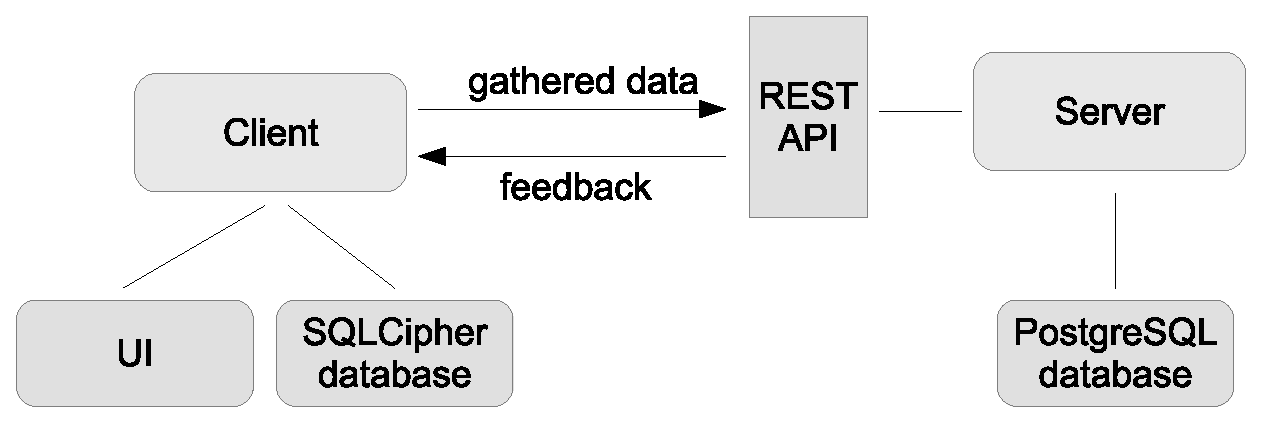
\includegraphics [width=0.7\textwidth]{images/Menthal_architecture}
  \caption{Menthal architecture}
  \label{fig:menthal_architecture}
\end{figure}

The client part consists of an Android application installed on a smartphone.
It keeps track of all the user activity during the day.
All the activities are stored as \textit{events}.
Each event contains such data as id, event type, timestamp, data itself and some additional information.
The main types of events are: SMS\_RECEIVED, SMS\_SENT, CALL\_RECEIVED, CALL\_OUTGOING, CALL\_MISSED, SCREEN\_UNLOCK, SCREEN\_LOCK, LOCALISATION.
The information gathering process is hidden from users, the application runs in the background, automatically sending data to the server.

The application gathers this data from different sources, using standard Android operating system API.
For example, to get the information about phone lock/unlock, it listens to the corresponding events and handles them.
To be aware of application usage, Menthal periodically (every 2 seconds) checks the current top application in the application stack of the smartphone.
If the application detects that the application has been changed, it writes the event into the database, adding a timestamp.
Catching a lock event is also used as a sign that the current application was changed and leads to a new record into the database.
The information about phone calls and sms can be queried from a local smartphone storage.
Every six hours Menthal checks whether the day is changed and if it does, it makes a new query to the local storage to get the latest information about performed calls and sent/received sms. 
 
\mnote{Menthal GUI}
Menthal has a user interface to provide users with a feedback. 
The main screen shows a 'score' - the relative phone usage measurement.
Using this value, one could check how intensively he uses his phone today comparing to previous days statistics.
UI provides also additional functionality.
It shows overall daily/weekly/monthly statistics about the phone usage such as most used application, number of calls or the number of times user unlocked the phone.
After a short questionary it can display personality characteristics diagram, that includes five sides: extraversion, neuroticism, openness, conscientiousness, agreeableness.
Furthermore a user can check the list of contacts with whom he communicates more often over a period of time.
The next screen shows the daily time spenditure with the phone for the last 30 days.
The application is able to keep track of user mood, periodically checking his current state of mind.
Using smartphone's GPS receiver, Menthal can determine and show on map the user location.
Moreover the application gives an opportunity to put a time limit on a particular application, so when the limit is exceeded the phone warns a user about that.

\begin{figure}[h]
\centering
\begin{minipage}{.5\textwidth}
  \centering
  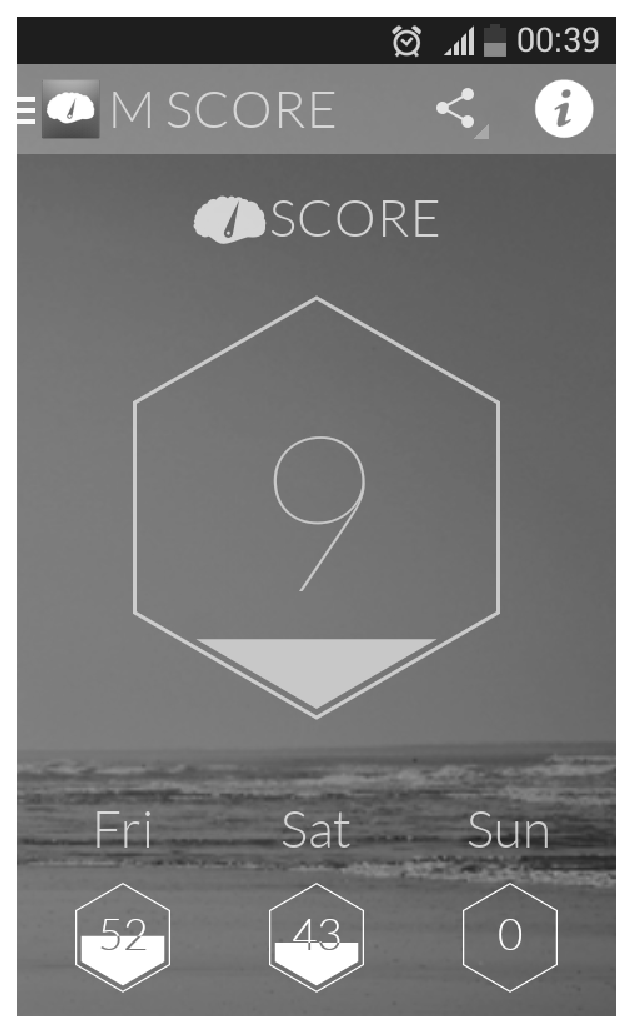
\includegraphics [width=.8\textwidth]{images/Menthal_GUI_mainscreen}
  \caption{Start screen}
  \label{fig:menthal_gui_mainscreen}
\end{minipage}%
\begin{minipage}{.5\textwidth}
  \centering
  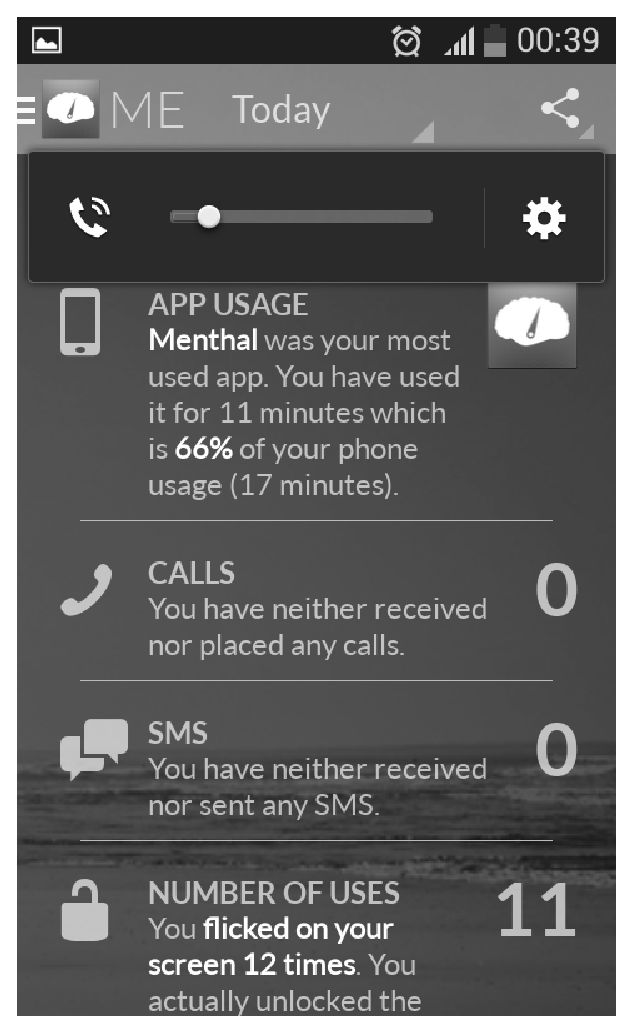
\includegraphics [width=.8\textwidth]{images/Menthal_GUI_me}
  \caption{Personal statistics}
  \label{fig:menthal_gui_me}
\end{minipage}
\end{figure}

\begin{figure}[h]
\centering
\begin{minipage}{.5\textwidth}
  \centering
  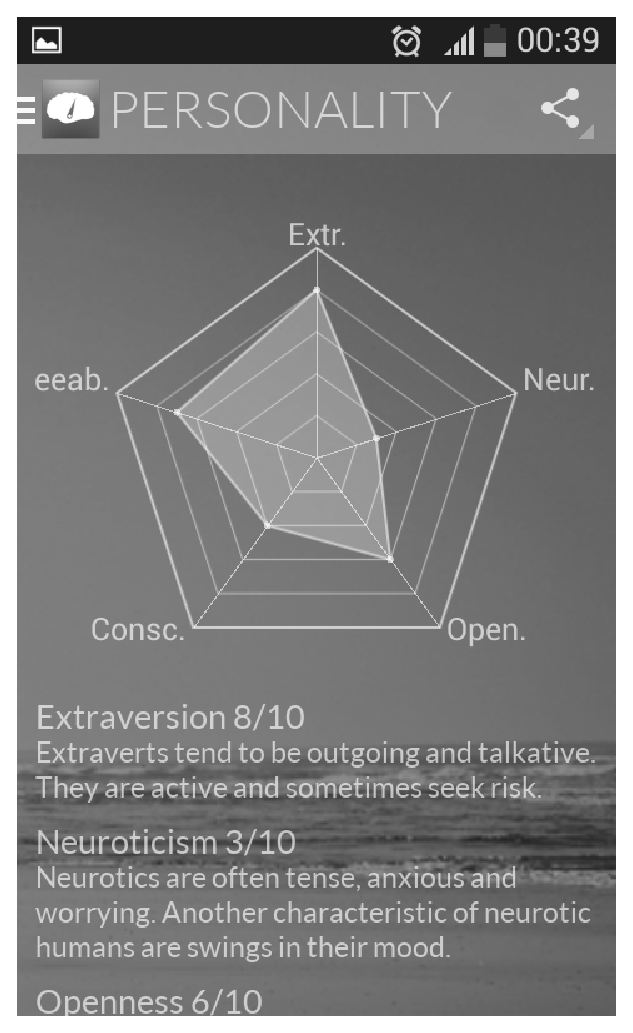
\includegraphics [width=.8\textwidth]{images/Menthal_GUI_personality}
  \caption{Personality characteristics}
  \label{fig:menthal_gui_personality}
\end{minipage}%
\begin{minipage}{.5\textwidth}
  \centering
  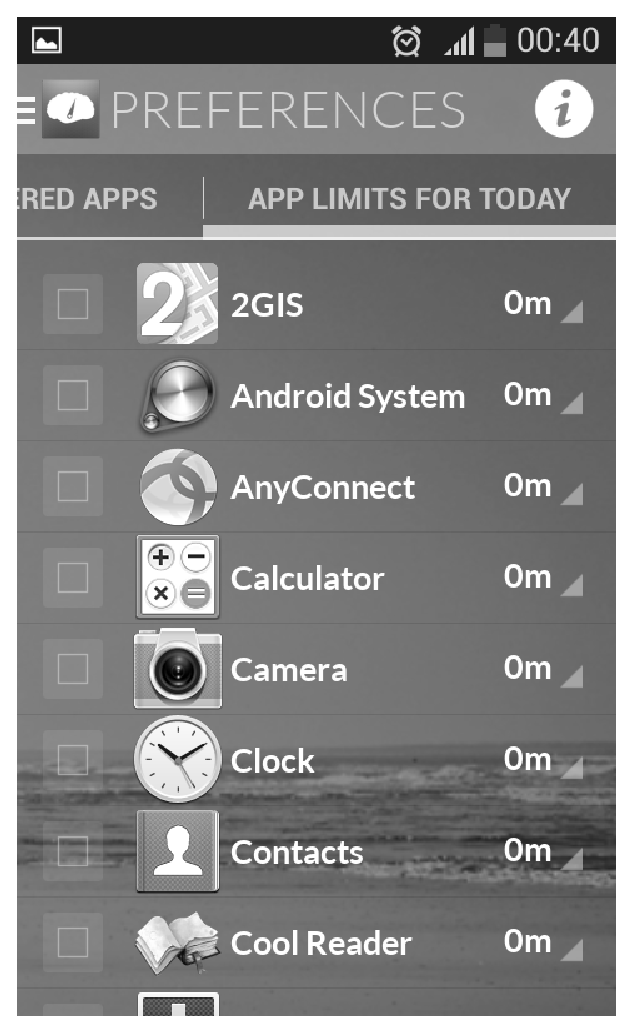
\includegraphics [width=.8\textwidth]{images/Menthal_GUI_preferences}
  \caption{Time limits preferences}
  \label{fig:menthal_gui_preferences}
\end{minipage}
\end{figure}

All the gathered data is temporarely stored on a phone in a cryptographically protected SQLCipher database.
Every time a new event is created, the application increases a special counter by 1.
When this value reaches 50, Menthal performs the following steps:

1) Obtain all the data from the SQLCipher database.

2) Convert it into JSON.

3) Send it to the server.

4) Wait for the reply.

5) If the server does not respose, try again in approximally 2 minutes. 

6) If the acknowledgment is received, delete the data that was sent from the SQLCipher database.

However, this is done only when a phone is connected to WiFi to avoid unnecessary charges for the user.
If the phone was not connected to WiFi during the day, Menthal still needs to send the data.
In this case the application sends it at random time between 1:00 - 6:00 at night via 3G.
All the data is sent in batches, where one batch contains no more than 50 events.

\mnote{information security}
Menthal uses secure connection, encryption of sensitive data and authentication mechanism to guarantee information security.
Communication between the client and the server goes through HTTPS.
This protocol is designed to provide a secure communication over a computer network. 
OAuth 1.0a protocol guarantees an authorization control.
When a client connects to the server the very first time, it receives a token.
Later the client sends this token with every message and the server uses it for authentication.
On the phone the data is stored in SQLCipher database.
This database uses 256 bit AES encryption for storing information in a secure way.
Moreover, Menthal hashes the sensitive data, such as the contact names or the phone numbers via SHA2. 

On the Server side Menthal has a cluster of 3 machines.
A PostgreSQL database is replicated between two of them.
One of these machines serves as a master node and another as a slave node.
The third machine hosts a key-value store that works as a read cache, message and task queues and a web application.
 
Menthal recently gained popularity among users.
It happened when the application was covered in mass media.
The articles in newspapers and interview with a project leader lead to the explosive increase of the number of users.
Almost 50 000 persons have this application installed on their phones.
All of these devices periodically send collected information to the server, that sums up to a vast amount of data.
Totally around 34Gb of information is received per day, that is almost 1Tb per month.
All these factors have a significant influence on the application performance.
The Menthal server side becomes overflowed and is not able to write all incoming data into database, not to mention providing a feedback.
Therefore, the application requires a new, enhanced server-side architecture that can meet the new requirements.
\chapter{Big Data Architecture [SP]}
\label{chap:big_data_architecture}

Traditionally, the process of making decisions is expensive and experiences significant error.
Simple reasoning is a straightforward approach, but it can work only till the certain point.
The main problem is that it can be easily ruined by the wrong assumptions.
Hence one would preferably use evidence based approaches that built on the accumulated data.
The most commonly used tools for this purpose are surveys and experiments, carried out on a control group.   
However, they both have significant disadvantages that makes the process of making decisions more complicated. 
On the one hand, surveys and experiments involve human resources, what leads to high expenses.
On the other hand, these approaches are also vulnerable to errors.
A lot of various reasons can cause an error, such as a survey composed in a wrong way, or a not representative control group.
 
Fortunately, this situation has changed dramatically in recent years.
First of all, data has become available for free, as a by-product of other processes (such as log files).
Moreover, constant reduction of data storage costs allows to warehouse enormous amounts of information, without troubling about the size limits.
Owing to the progress in the information technologies area, both transferring and processing of huge data volumes become easy.
All this gives us an alternative solution to the problem of making decisions that avoids the drawbacks of the strategies presented above.
The name of this solution is Big Data.

The main distinguishing feature of Big Data is that data collection is independent of use case.
Information is collected because it is available and cheap, with the hope that later on it can be used to answer a question that has not arisen yet.
For example, Facebook stores all available data about the users, like demographic information, geographic location, connections with other users, visited websites, clicked links, etc.
As a result it has a huge amount of data, which, with the right approach, can give lots of useful information. 
For instance, afterwards it can be used in targeted advertising, or for performing the social network analysis.

\section{Big Data}
\mnote{Big Data}
There is no consensus about the origins of the term "Big Data", but most of the sources claim that it is first mentioned in the press in 2008.
People start actively using it since 2009 and it spreads quickly owing to its precise and capacious meaning. 
Big Data is characterized by its high (i) variety, (ii) velocity and (iii) volume. [reference - find from wikipedia]
All these three "v" constitute a criterion that allocates Big Data observation into a distinct sector of computer science, which requires ad hoc decisions and a special approach.

\mnote{Variety}
First, Big Data sources are highly diverse.
They differ in the type of produced data - it can be text, images, sounds, raw feed incoming directly from sensors, etc.
Each of these types, in turn, may have a different format.
For instance, text can be transmitted in various languages, coding, formatting and so forth.
Big Data sources also differ in the speed of data flow and the data purity.  
Some of the sources generate noisy information, while others can produce data, that does not need cleaning.
Moreover, Big Data differ in the way how it is collected, how urgently it should be processed and which storage capabilities are available for its warehousing.

\mnote{Velocity}
The diversity of Big Data sources causes the high velocity of data input flow.
For example, Menthal, mentioned above, currently receives data from 50 000 users.
It sums up to almost 30Gb input data per day.
Therefore, Menthal reseives on average around 24Mb per minute, that sends a challenge how to handle input data flow on such a hight speed.

\mnote{Volume}
In the end, massive sources variety, multiplied by high velocity of data generation, results in its enormous size.
For instance, by the end of 2013, the number of Facebook users reaches 1.23 billion.
Each of them not only has some profile information, but also communicates with other users, shares data, updates the timeline and so forth.
In total 2.5 billion content items are shared every day.
Let us assume that each of these events is stored as a JSON object and needs 2Kb on average.
That means that in the end of the year Facebook deals with 4.65Tb * 365 = 1.65Pb of information.
And it is only metadata, not including images and video files that require significantly more space. 
As a result, Facebook deals with storing and processing petabytes of data.

Another example is the information received from sensors.
Sensor is a converter that measures and transforms physical quantity into a digital signal.
Sensors find an application in various fields: manufacturing industry, transportation systems, meteorology, medicine, even modern smartphones have lots of sensors.
The key feature of a sensor is that often it does its job constantly, continuously producing the flow of information, what leads to the large volumes of data.
Nest Labs is an American company that manufactures sensor-driven thermostats and smoke detectors.
The population of United States is about 318 million, so if every hundredth resident uses at least one of Nest thermostats in the house, it sums up to 3.2 million devices.
One thermostat has a variety of sensors, like activity, temperature, humidity, illumination, etc.
Each thermostat generates and transmits around 2Mb of data per day.
Consequently, all Nest thermostats in United States generate around 2.17Pb of data per year. 
The ability to process large amounts of information is the main benefit of Big Data analytics, since with its vast volume it is possible to construct better models.

\mnote{Batch Processing}
There are two fundamentally different ways of processing the Big Data, namely Batch and Real-Time data processing.
In the first case, data is handled in batches, i.e. process collects the data until the batch size is obtained, and only after this the process can perform the necessary actions on a batch as a whole.
This gives several advantages.
Batch processing can be done in the appropriate time, when the computing resources are less busy.
Furthermore, one can set a priority for each task, beginning with more urgent operations.
There is no need in a close supervision of a run, batch processing is mostly autonomous.
Finally, it becomes possible to process multiple operations in one request, instead of handling each operation individually.
That makes data treatment more efficient. 

To give a naive example how batching improves the performance, let us describe the problem of I/O operations.
For instance, an application every second receives data that should be written to the hard disk. 
There are two options how to implement the writing procedure.
On one hand, an application can write the input data every time it receives it, i.e. in our case every second.
On the other hand, it is possible to accumulate input data in memory until it reaches the defined size and than write the whole batch at a time.
It is known that I/O operations involve physical movement of mechanical devices (e.g. seek motion of hard drive).
Thus, the speed of sequential writes to a file is higher than random writes, because in the latter case additional time is spent for seek operations between each write.
This means that in our simple example the second option is preferable, because it decreses the number of seek operation and therefore makes the writing faster.    
The same principle also works in general case, i.e. combining multiple operations in one batch can significantly enhance performance.
However, Batch processing has one significant drawback: the results are always obtained with an arbitrary time delay.

\mnote{Real-Time Processing}
Real-time processing handles data at the moment of arrival. 
The advantage of the latter is that the results are ready almost immediately, which can be an essential requirement in such areas as medicine or security threat prediction. 
In spite of the fact that a certain delay is nevertheless exists, its duration is predetermine and is guaranteed to have a specified value.
That differentiates real-time processing from batch processing.
This fixed delay length varies depending on the application.
In some cases 10 minutes to perform all the computations is still considered to be a real-time processing.
However, in other cases, more than 1 second delay is unacceptable.
Real-time processing makes the information always available and up-to-date.

These significant advantages results in rising popularity of real-time processing, despite the fact that it requires greater effort to design and maintain.
Real-time processing can help to improve traffic in metropolitan areas, offering various travel alternatives for a vehicle, basing on analysis of incoming data about the situation on the roads.
Rapidity of data processing can be necessary in other cases as well.
Sometimes high processing speed can even be indispensable to life, when using in medicine, for example.
Special systems monitor the state of a patient, immediately alerting caregivers in the case of dangerous anomaly occurrence. 

\section{Architectural Requirements [SP]}

%System must provide information having gathered data from users and other sources.
%Application of complex algorithms is often necessary.
%Amount of data and rate of its arrival are heavy.
%Those aspects makes system to preprocess indices and aggregations that provide useful information.
%Batch processing is a good solution for that, nevertheless it has a drawback - execution time is long.
%Incremental processing resolves this issue.
%In combination these two approaches allow to design a system, that answers user queries with low latency as well as high accuracy.

%The purpose of the system is to answer queries having data.
%Let's consider an artificial example.
%Suppose we have a website where people pose programming questions, and other answer them.
%In this case the simplest query to the system is to return list of answers for a particular question post.
%Another query is to find all posts containing given keyword.

%One query is easy to answer, another requires application of complex algorithms.
%It is pretty easy to get list of answers to the question post having its id.
%You simply create hash-table that maps questions' ids to lists of answers' ids.
%Search by keyword, or even phrase search, is much more complex.
%To make it possibe we have to build specific inverted index, and this requires much more time to execute and to programm.
%Let's further assume, that our system has to provide keyword search, using precomputed inverted index. 

%Amount of data gathered with the time, as well as intense of arrival, can be huge.
%Let's consider again our example website.
%Assume that on average every second 5 questions and 20 answers appear.
%Every post is about 100 words, each of about 8 unicode symbols.
%The rate of incoming data is then $25*100*8*2=39$ KB per second.
%It is about 3.2 GB per day.
%This leads our system to be able to process such amount of data efficiently, as well as to rapidly reflect the state of inverted index with newly arrived posts.


There are some requirements that are common for most of the Big Data architectures.
Big Data systems deal with a large volumes of information, that constantly growth, therefore a system should be highly scalable.
Scalability has a direct impact on performance, thus it is essential to maintain a system performance on a proper level.
Moreover, availability and reliability are important attributes of a distributed architecture.
All these properties are described in the following paragraphs.

\mnote{Performance}
Performance is a quantitative characteristic of operation speed.  
This concept includes a variety of aspects, such as response time, processing speed, latency, bandwidth, etc.
With regard to extremely high volume and velocity of Big Data the question of system performance is a big issue.
For fair comparison of multiple systems performance a benchmark is used.
A benchmark is a sequence of tests that helps to estimate the performance of the system.

\mnote{Scalability}
Scalability indicates the property to handle an increasing amount of work.
It means that the performance of the system can be enhanced using additional hardware resources.
There are two types of scaling, namely vertical and horizontal.
Vertical scaling means that the single node of a system is enriched, e.g. CPU is added to a computer. 
Horizontal scaling denotes the enlargement of a system by adding new nodes.

\mnote{Commodity hardware}
In the context of Big Data architecture the latter method is of great interest for us.
First, in some cases the system should be distributed geographically.
For instance, adding new nodes closer to the customer can reduce the network load.
Second, because of the decreasing computer price it becomes possible to build highly performant systems using commodity machines.
A commodity computer is a moderately priced machine that is widely available for purchase.
The usage of inexpensive hardware helps considerably decrease the cost of the system.
It is especially relevant in the context of Big Data because of its overwhelming scales.
One of the well-known examples is the Google Lego server.
In 1996 two students, Larry Page and Sergey Brin, needed a cheap but capacious server to test the Pagerank algorithm on a huge data. 
[picture?]
They assembled it using 10 drives 4Gb each and a Lego enclosure. 
Nowadays Google uses commodity computers for building their computing clusters.

\mnote{Fault tolerance}
The direct consequence of the cheap hardware is the high failure rate.
Moreover, the large number of components also increases the probability of failure. 
Thus the system should be highly fault tolerant, with timely error detection and easy automatic recovery.

\mnote{Large files}
The world of Big Data introduces its own specific requirements for architecture design.
The file size can be enormous comparing to the standards.
It is not rare to work with a file of several gigabytes.
Storing the data in large files simplifies data processing.
The size of data itself is huge and it is more efficient to work with several large files than with great number of small files.

There are two metrics to measure the robustbness of a system, namely availability and reliability.
At first sight they look similar, however these two metrics assess a system from different perspective.
\mnote{Availability}
Availability means that a system operates properly at any given moment.
It can be calculated by the following formula: (total time - down time)/total time.
Consequently, availability depends on the sum of the time the system was down.
That means that even if the system fails every hour, but for negligible time, it is still considered to be highly available.

\mnote{Reliability}
In contrast, reliability denotes the capability of a system to operate continuously without failing.
Reliability and availability are the opposite concepts.
The highly available system mentioned above is not reliable, because the intervals of working without failing are relatively short.
However, the system that is down for one hour but only once per month can be reffered to sufficiently reliable.

Big Data architectures have to be targeted to each specific scenario.
For instance, architecture, designed for processing video data from a web camera, differs significantly from one for handling server log files.
Menthal, mentioned in Chapter 2, deals with data, that consists of a bulk of key/value pairs. 
As a result, Big Data technology becomes an umbrella of various systems. 
Data has to be collected, processed, transmitted, stored, protected from attacks, etc.

The Figure~\ref{fig:big_data_flow} shows the general flow of data within the Big Data concept.
Each of the presented steps involves a batch of technologies.
For example, depending on data type and size, one can choose SQL (MySQL, Oracle, Teradata, etc.) or NoSQL (Cassandra, MongoDB, Apache HBase, etc.) solutions for storing Big Data.
Similarly, depending on the application, Real-Time processing (Storm, Spark Streaming, etc.) or Batch processing (Apache Hadoop, etc.) technologies are used. 
Thereby, it is apparent that no one general solution exists for every Big Data problem.
Further we describe the existing Big Data architectures in the context of Menthal needs.

\begin{figure}
  \centering
  \includegraphics [width=0.8\textwidth]{images/big_data_flow}
  \caption{Big Data Flow}
  \label{fig:big_data_flow}
\end{figure}

\section{Naive Approach}
\mnote{PostgreSQL}
It is natural to start with a naive approach, using widely available and easy to use technologies.
As a storage system, one could use a relational database, such as MySQL or PostgreSQL.
PostgreSQL is an object-relational database management system.
It is an open source project, that is quite popular among developers due to its high security standards, good performance and scalability.
PostgreSQL was chosen as a database for Menthal application as a compromise between widespread but primitive MySQL and such large-scale solutions as Oracle or MongoDB.
On the one hand, it supports sufficiently complicated queries and easily scales, comparing to simple MySQL database.
On the other hand, it is not overload with redundant functional and does not require high maintenance affords as large-scale database management systems.

\mnote{REST}
Menthal uses a Representational state transfer (REST) API for communication between client and the database.
In this context RESTful API means that all the required information is transferred as parameters inside of an HTTP request (GET or POST).
The application uses stateless type of data exchange, that means that the server does not store a client state.
It helps to decrease the load on the server side, however increasing the amount of exchange traffic.
This straigforward approach is easy to implement, however, at a certain point, it cannot anymore sustain a constantly growing load.
The datatbase cannot cope anymore with the increased input flow, returning a timeout error.

\mnote{Database mirroring}
Database mirroring avoids the database overload.
It is a technique of keeping redundant copies of a database.
It enhances data availability and allows to always have an accessible copy of a database on one of the machines.
There is a special kind of mirroring called a hot standby, when every change is copied immediately to the mirrored instance.
In this case, there is a guarantee that all the instances keep the identical data, however, it can lead to a high latency.
If some data loss is permitted, a warm standby mode can be used, when the data is not fully synchronized across the database instances.
It does not grant the same information consistency as a hot standby mode, but it shows better performance results.

\mnote{Database caching}
Database caching is another technique for improving architecture scalability. 
In this case data is cached in high-performance store, e.g. in memory.
The access to memory is faster than the reading from a file or a database or transfering data via HTTP.
When the application often uses such external resources, database caching significantly increases performance. 
The drawback of both approaches is that they only improve reading, leaving the problem of large-scale writing unsolved. 

\mnote{Sharding}
In this situation it is reasonable to use horizontal partitioning, also known as sharding.
Sharding helps to enhance write scalability.
It denotes the process of partitioning of database tables by rows.
Each partition (shard) can be settled on separate machine.
This technology allows to spread the write load between multiple database servers.
Also it reduces the index size, thereby improving performance.
However, with growing input flow, the maintaining of shards and auxiliary infrastructure becomes more and more complex, demanding too much effort from developers. 	   
Hence the biggest IT corporations conduct their own research in this area, designing specific architectural solutions for working with Big Data.
\chapter{Industrial Approaches [SP]}
\label{chap:google_architecture}

Google is one of the well-known examples of corporations that deal with Big Data.
Its activity directly relates to storing and processing of large volumes of data.
Google Search engine handles more than three billion searches every day.
Social networking service Google+ had 540 million users in 2013.
Gmail, Google's email service, had 425 million users in 2012.
These are just several examples of large-scale Google projects, that processes huge amounts of data.
Therefore, Google introduces a batch of solutions for building scalable systems. 

The overall structure of Google Big Data architecture is presented on the
Figure~\ref{fig:google_architecture}.
The lowest layer is Linux kernel, that serves as a basis for Google File System.
Google File System is a scalable and highly available file system. 
These properties are achieved by replicating data across several machines.
Next, data can be efficiently processed by MapReduce framework.
This technology includes two steps - map, that performs filtering and sorting and reduce, that aggregates the output of map step to the final result.
Bigtable, a highly scalable database, provides a way to store massive amounts of information.
Finally, client application uses these technologies to perform highly scalable and distributed tasks.  
Let us explain in more detail the primary features and internal structure of these technologies.

\begin{figure}
  \centering
  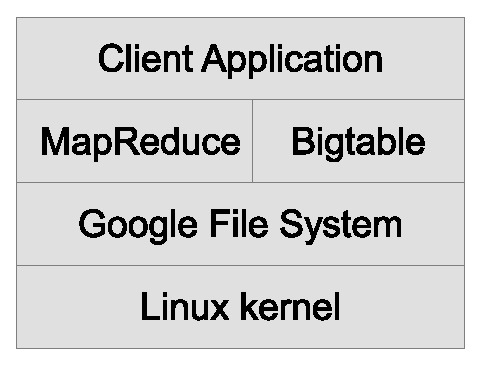
\includegraphics [width=0.4\textwidth]{images/Google_architecture}
  \caption{Google Architecture}
  \label{fig:google_architecture}
\end{figure}

\section{Google File System}

[reference]
\mnote{Google File System}
Google File System (GFS) is a scalable distributed file system, which supports Big Data operations.
The underlying idea is the following: Google Search Engine and some other Google systems process vast amount of data, which is spread all over the world.
Hence the file system should be highly extensible, give an opportunity to use cheap hardware components and, consequently, be fault tolerate. 
Furthermore, it has some specific usage features.
Because of vast scales and cheap hardware, component failure is a commonplace.
The size of files exceeds several-fold the traditional standards, so a multi-gigabyte file is not unusual.
Most of the time the stored data stays unchanged and new data is only appended.
The append operation, in its turn, should provide the concurrent access for multiple clients.
GFS architecture design helps to meet all these requirements.

The Figure~\ref{fig:GFS_architecture} illustrates the main components of the GFS
Architecture.
Each GFS cluster contains one master server and several chunkservers.
The master has a "shadow" node, that provides read-only access when the primary master is down. 
Chunkserver stores chunks as Linux files on local disk.
Every chunk is replicated on several chunkservers for reliability.
One chunk combines multiple files and has a fixed size of 64 megabytes.

% Figure: according to [66]
\begin{figure}
  \centering
  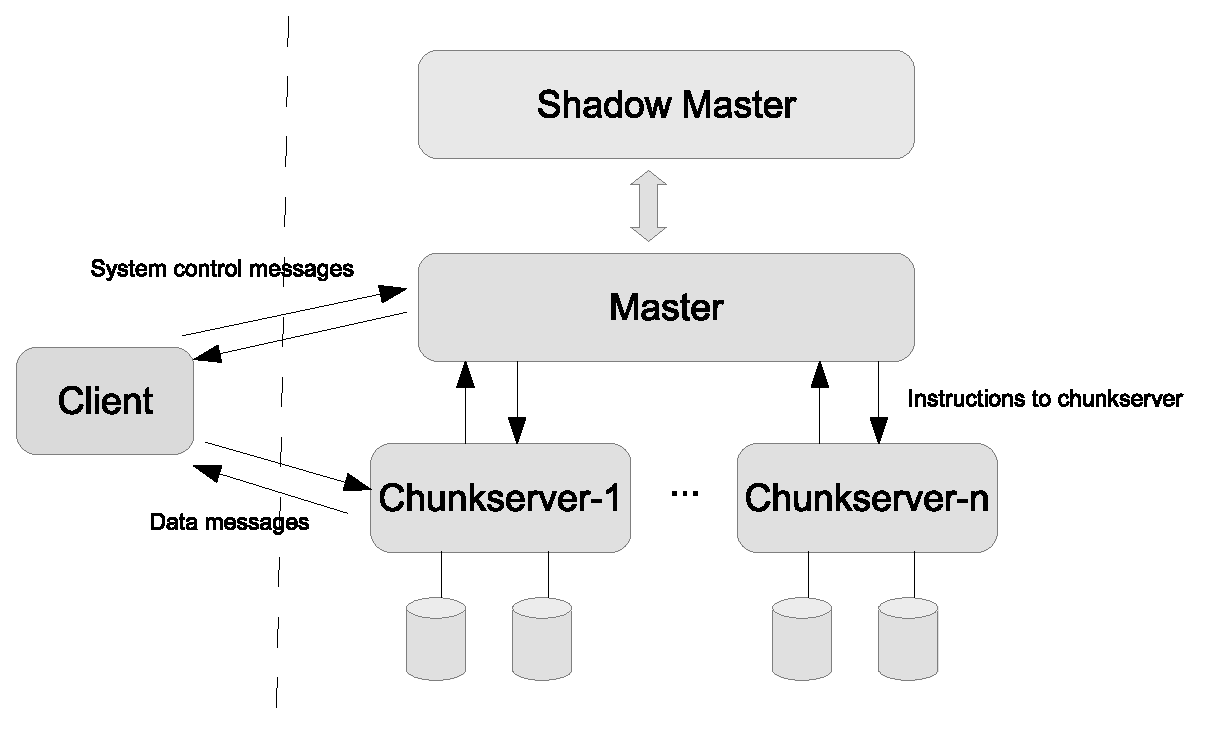
\includegraphics [width=0.8\textwidth]{images/GFS_architecture}
  \caption{GFS Architecture}
  \label{fig:GFS_architecture}
\end{figure}

The large size of chunk gives several advantages.
Clients send requests to the master for chunk location less frequently.
A persistent TCP connection to the chunkserver for a longer time period allows to avoid network overhead.
The master node stores less metadata that provide a possibility to keep it in memory.

The master node manages the mapping from files to chunks, location of chunks, access control, garbage collection and some other tasks.
It does not persistently store the information about chunks location. 
On the contrary, it gives instructions to chunkservers and collects their states using periodic HeartBeat messages.
To prevent the master being a bottleneck, only file system control data goes through it.
For example, a client can ask the master node which chunkservers it should contact.
The master node returns the corresponding chunk handle and its replicas' location.
After receiving a reply, the client caches this information and can directly transfer data to the given chunkserver, dispensing master node from overload.
Clients and chunkservers do not cache file data.
Clients mostly work with files that are too large to be cached.
Chunkservers treat chunks as Linux files, therefore in this case caching is done by operating system.

\mnote{Operation Log}
To recover its state, the master uses the operation log.
The operation log consists of the chronometric information about critical metadata changes.
This log is replicated on several machines.
For the purpose of consistency, client receives a respond for operation only when corresponding log record is flushed to a local disk and the disks of all replicas.
To avoid the operation log being too large, the master makes a checkpoint each time when the log size exceeds a certain threshold.
In the case of failure, the master can load the latest checkpoint from local disk and replay it, recovering its state.
For storing checkpoint it uses a compact B-tree like data structure, that allows to map it directly into memory and perform fast lookups.
For performance reasons the new checkpoint is created in separate thread.
The ability of a server to restore its state does not depend on the way it was terminated.
Shutting down a server by killing the process is a normal procedure. 

\mnote{Mutation}
A mutation denotes a change of the contents or metadata of a chunk.
There are two types of mutations, namely writes and record appends.
In the former case data is written with a file offset specified by a client.
In the latter, GFS chooses an offset, and data (record) is appended with an append-at-least-once semantics.
Record append operation is atomic, i.e. it is treated as one continuous sequence of bytes. 
This allows multiple clients to append information concurrently.

\mnote{Lease}
Each mutation is replicated across several chunks.
To keep a mutation order consistent at all the replicas, GFS uses a technique of leases.
The master gives a lease to one of the replicas, that becomes a primary replica.
The primary chooses an order for all the chunk's mutations and each replica then follows this order when applying mutations.

The flow of write control is shown on the Figure~\ref{fig:write_control_flow} in
more details.

\begin{figure}
  \centering
  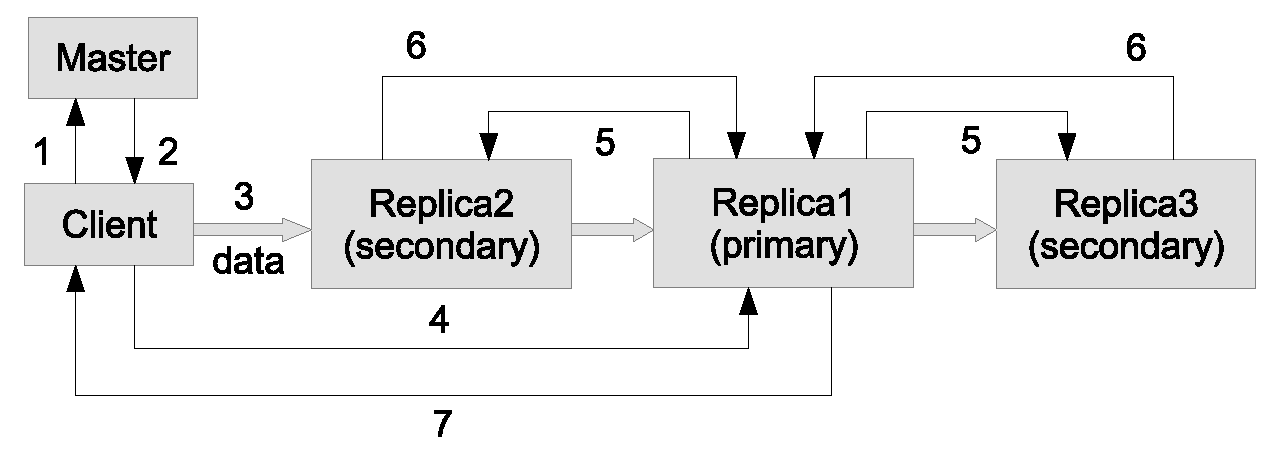
\includegraphics [width=0.7\textwidth]{images/write_control_flow}
  \caption{Write control flow}
  \label{fig:write_control_flow}
\end{figure}

1. The client sends a request to the master.

2. The master replies with a chunkserver, that holds the current lease, and the location of the other replicas.
If a primary replica (that has a lease) is not defined, the master chooses one. 
The client caches this information for the next mutations.

3. The client sends the data to all the replicas in arbitrary order.
Chunkservers store this data in an internal buffer cache. 

4. When the client receives acknowledgements from all the replicas, it sends a write request to the primary.
The primary picks serial numbers to all the mutations it has received and performs them in corresponding order.

5. All secondary replicas receive the write request forwarded by the primary.
Each replica applies mutations to its own state in the same order assigned by the primary.

6. The secondaries notify the primary about the completion of the operation.

7. The primary sends a reply to the client.
In the case of error occurrence at any of the replicas, the primary informs the client about them.
The write is considered to be successful, if the primary and an arbitrary number of secondary replicas succeeded.

GFS differs from traditional file systems in the way how it manages files and directories.
There is no possibility to list all the files in a directory in GFS, because it does not support per-directory structure.
It stores a mapping between full pathnames and metadata in a lookup table.
Prefix compression helps to efficiently represent this table in memory. 

The file deletion does not occur at once.
Firstly the master logs the event of deletion.
Than the system renames the file with a hidden name that includes the time of deletion.
The master performs a regular scan of the namespace and removes a hidden file, if it has existed for more than a specified time interval (e.g. 3 days). 

All the described features help the Google File System to successfully cope with a large-scale data processing workload.
GFS meets the storage needs of Google corporation.
Therefore Google uses GFS as the storage platform for many applications, both in research and production areas.
Another Google technologies, like MapReduce or BigTable are based on it.  	 

\section{MapReduce}

\label{sec:mapreduce}
[reference]
MapReduce model finds wide application in a variety of real world tasks.
For example, search engines use web crawling to gather a vast amount of information.
They process this information to create inverted indices, construct web graphs, figure out the most frequent search queries, etc.
Any of these tasks can be divided into two steps, namely Map and Reduce.
Map operation converts input data to a set of intermediate key/value pairs.
Reduce operation, in its turn, combines all the values that share the same key.
The advantage of the MapReduce abstraction is that it hides the implementation details from users.
This allows even not experienced programmers to easily construct parallel and distributed systems.

MapReduce shares the same requirements with other systems that work with large data sets.
It should provide high parallelization, be fault-tolerant and perform load balancing between nodes.
Applying Map and Reduce operations helps to parallelize large calculations.
Moreover, this makes simpler re-execution of a task that serves as a primary mechanism for fault tolerance.

Both Map and Reduce operations work with key/value pairs.
The user of MapReduce library determines the logic of these operations, specific to the given application.
The Map function receives an input a key/value pair and produces a set of intermediate pairs.
The MapReduce library groups these intermediate pairs together by the key and passes the result to the Reduce function.
It passes them via iterator that allows to handle a large data set without keeping it in memory.
The Reduce function merges the values with the same key, possibly decreasing a given set of values.
One Reduce function invocation most of the time produces a single output value, or even none.
A pseudo-code for a simple MapReduce task is illustrated in Listing~\ref{lis:simple_mapreduce_task}.

\begin{lstlisting}[float=h, caption=Simple MapReduce task, label=lis:simple_mapreduce_task]
def map(key, value):
	list = []
	for x in value:
		if some_condition_holds:
	 		list.append((key, x))
	return list

def reduce(key, list_of_values):
	result = 0
	for x in list_of_values:
		result += x
	return (key, result)
\end{lstlisting}

\begin{figure}
  \centering
  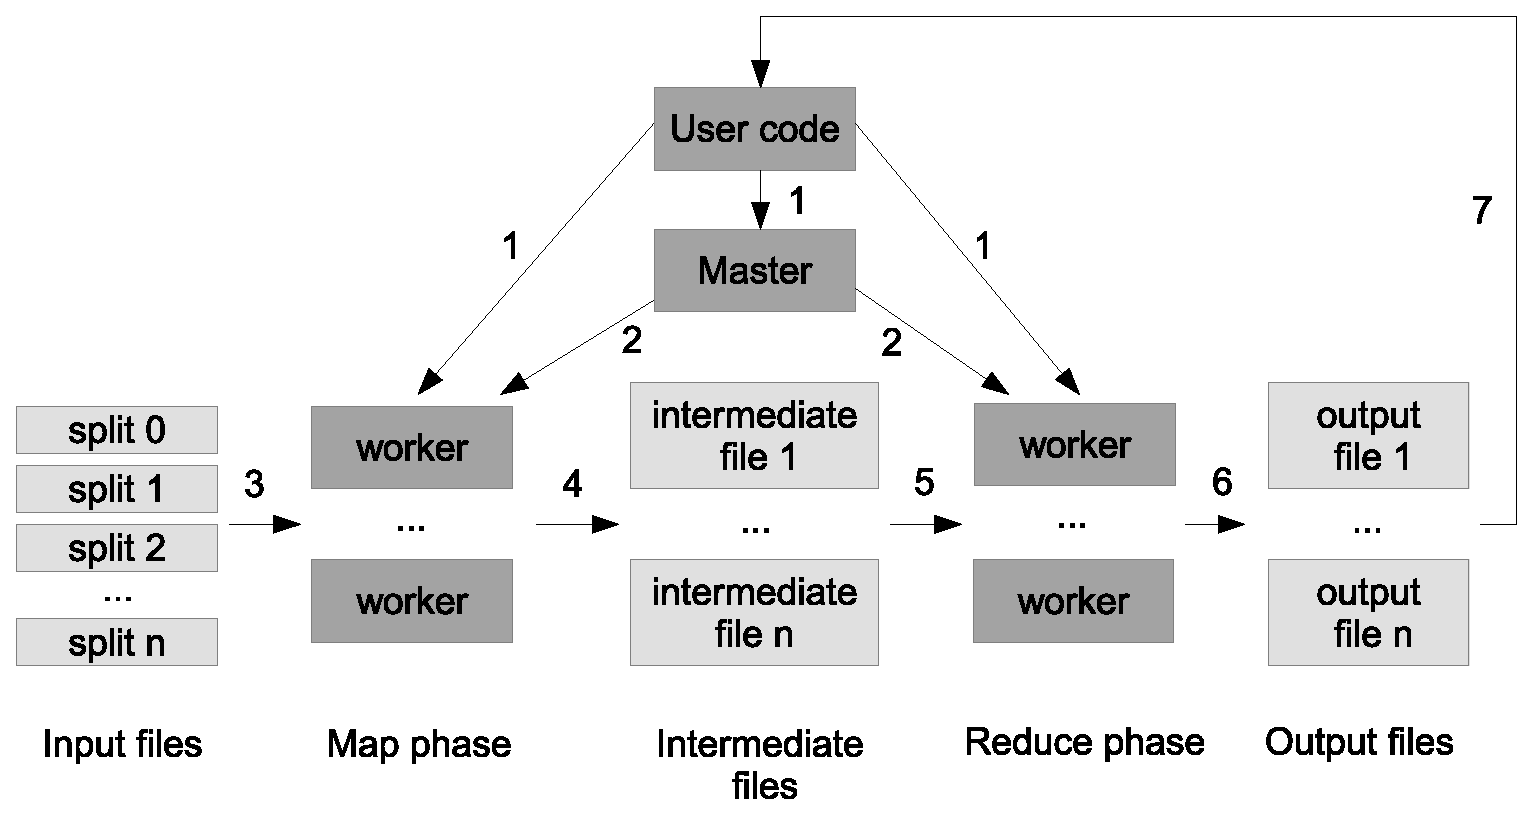
\includegraphics [width=0.9\textwidth]{images/MapReduce_operation_flow}
  \caption{MapReduce operation flow}
  \label{fig:mapreduce_operation_flow}
\end{figure}

We visualize the overall flow of a MapReduce operation in the Figure~\ref{fig:mapreduce_operation_flow}.

1. The MapReduce library divides the input files into M splits.
The size of one piece varies from 16Mb to 64Mb depending on the chosen settings.
User code invokes the MapReduce routine on several machines.

2. One of these machines is a master, while others are workers.
The master manages the workers, assigning to idle nodes one of M map tasks or one of R reduce tasks.

3. A worker that handles a map task reads the data from a respective input split.
It passes the parsed key/value pairs to the Map function.
The intermediate output of the Map function is stored in a buffer.

4. The MapReduce library periodically writes the buffered data into selected number of R local intermediate files.
Also it informs the master about the location of these files.

5. The master passes the locations to workers that handle a reduce operation.
A reduce worker reads the intermediate pairs from a specified location using remote procedure calls.
After compliting the reading, the worker groupes together all the pairs that share the same key.

6. These pairs are then passed to the Reduce function, one key and one or several related values at a time.
The output of the Reduce function is written to one of the output files.

7. After finishing all the map and reduce tasks, the MapReduce library returns the control to the user code.
The derived output files can be directly processed or be used as an input to another MapReduce task.

The MapReduce library has an optional Combine function that can be used for optimisation.
For example, let us consider the task of counting the number of words in English text.
Most probably it contains a lot of articles `a` and `the`.
Each Map task sends thousands of pairs <a, 1> to a single Reduce operation over the network. 
The Combine function can improve this situation by partial merging these pairs before sending them over the network.
Each machine that executes a Map function now also executes a Combine function.
Combine operation often uses the same code as Reduce one.
The difference is that the output of the former is stored in an intermediate file, while the latter writes it into the final output file.

The usage of Google File System (GFS) for storing input data helps to reduce the network bandwidth consumption.
GFS stores input data in blocks, copying each block on different machines (usually it makes 3 copies).
The master in MapReduce library knows which machine contains a replica and tries to assign a corresponding map task to this machine.   
When it is not possible, the master uses the nearest node to that machine.
This technology conserves network bandwidth significantly, especially when dealing with huge MapReduce operations.
 
The master keeps track of worker failures.
For this purpose it stores the state of each task and the identity of the worker that performs the task.
There are three types of states: idle, in-process and completed.
The behavior of the master in the case of failure depends on the type of the task (map or reduce) that failed.
When the map task fails, the master re-executes it on another worker.
Re-execution is required since the output of the map task is stored locally on the failed machine.
On the contrary, there is no need to re-execute the reduce task because global file system stores its output.
Sometimes a failure is caused by a defective record.
In this case the MapReduce library optionally can skip this record to continue the work. 
 
Stragglers is another problem that can obstruct the task completion.
Straggler is a machine that handles the last several map or reduce tasks too slow, keeping the whole system waiting for completion.
The MapReduce master uses a special mechanism to solve this problem.
On termination of an operation it executes the remaining in-process tasks on two different machines.
When either primary or backup worker completes computations, the task is considered to be completed.

Google Search engine widely uses MapReduce functionality for indexing, computing different statistics and analysing data.  
Moreover MapReduce can significantly facilitate the problems of data mining and machine learning.
Its key feature of dividing the computation into Map and Reduce phases helps to easily build distributed systems and makes the computation considerably more efficient.  

\section{BigTable}

[reference]
Some Google projects deal with so large amounts of data, that common storage systems cannot sustain such a load.
For instance, personalized search, that stores user browser history and handles search queries based on the stored information about user activity.
It is necessary to warehouse each user's data.
Taking into account the huge number of Google Search users, the amount of data to be stored is also tremendous. 

The company introduces its own storage system for these purposes - a Bigtable.
It is a sparse, distributed, persistent multidimensional sorted map. [reference]
Bigtable uses three-dimensional mapping: row key, column key and timestamp are mapped to an array of bytes.
It is created to store petabytes of data in a distributed way.
As Google uses Bigtable in various projects, it puts different requirements on data size and latency of the storage system. 

\mnote{row keys}
The row key is represented by an arbitrary string with a maximum size of 64Kb.
Read and write operations under one row key are atomic.
Bigtable stores row keys in lexicographic order and dynamically partitions each row range.
One partition is called a tablet and serves as a distribution and load balancing unit.
For instance, when storing web pages with an URL as a row key, it is optimal to arrange pages from the same domain in one tablet.
In this case an URL like en.wikipedia.org/index.html is presented as org.wikipedia.en/index.html.

\mnote{column keys}
Bigtable groups column keys into column families, which serves as an access control units.
It means that each column family can have different access permissions (e.g. write access for one application and read only for another one).
It is common to store in one column family data of the same type.
One can store data under a column key only when a column family comprising this column key is created.
Number of distinct column families should be kept small, while each column family can contain unbounded number of columns.
The name of column key is presented as family:qualifier pair, where family should be printable and qualifier can be an arbitrary string.
For example, the column key name can look like language:en, where 'language' is a column family name and 'en' is a language ID. 

\mnote{timestamps}
Timestamps are used to store multiple versions of the same information.
A timestamp can be assigned in different ways.
On the one hand, Bigtable can use the time in microseconds as a timestamp.  
On the other hand, a client application can maintain its own unique timestamps.
Several versions of data are ordered such as the most recent version can be accessed first. 
Garbage collector processes the outdated data automatically using one of the two column family settings to detect the outdated versions.
The first setting allows to keep only the last \textit{n} versions of data, while the second setting allows to keep data that was written in the last \textit{m} days.

\mnote{Sawzall}
Bigtable allows user to manipulate the stored data using a special language developed by Google.
The language is called Sawzall.
Scripts, written in this language, can execute on Bigtable server's address spaces.
Using Sawzall scripts one can filter, transform and make various summarization on data.

\mnote{Chubby}
Chubby is a persistent distributed lock service for synchronizing access to shared system resources.
The Chubby service replicates to five nodes, choosing one of them to be a master node.
The service provides a namespace, that contains directories and files, and uses them as a lock.
Chubby has a client library that can keep the cached Chubby files in memory.
Every client sustains a session with Chubby service.
The expired session loses all the locks.

Bigtable uses Chubby for several purposes.
First, Chubby guarantees to have at most one active master at a time.
Second, it handles the appearance of new tablets and finilizes the dead ones.
Third, it stores the schema of Bigtable and access control lists.

The major components of Bigtable are a master server, a number of tablet servers and a library linked into each client.
It is possible to dynamically add or remove tablet servers according to given workload.
The master assignes tablets to tablet servers, performs load-balancing, garbage collection.
Furthermore, it is responsible for creation of tables and column families.
Each tablet server controls a tablets set.
When a client sends a read or write request to the tablet, this request is processed by the tablet server.
Also the tablet server splits too large tablets.

The internal details of master-slaves interaction are similar to those mentioned above in GFS and MapReduce subchapters.
Analogously, the system does not transfer client data through the master and establishes a direct connection between clients and tablet servers.
It prevents the high load of a single master node.

A Bigtable cluster warehouses one or several tables.
A table contains a number of tablets. 
All the data that belongs to one row range is situated in one tablet.
Primarily one table contains only one tablet.
When the table becomes larger than a specified threshold, it automatically splits into several tablets.

\mnote{METADATA table}
The root tablet uses a special METADATA table to store the location of tablets.
The root tablet is a first tablet in this table.
However, it is never split in contrast to the rest of the tablets to keep the number of hierarchy levels constant.
Figure~\ref{fig:bigtable_tablets_hierarchy} illustrates the tablets hierarchy.
The METADATA table also stores logs of operations on each tablet.
This data can be used for preformance analysis and debugging.  

\begin{figure}
  \centering
  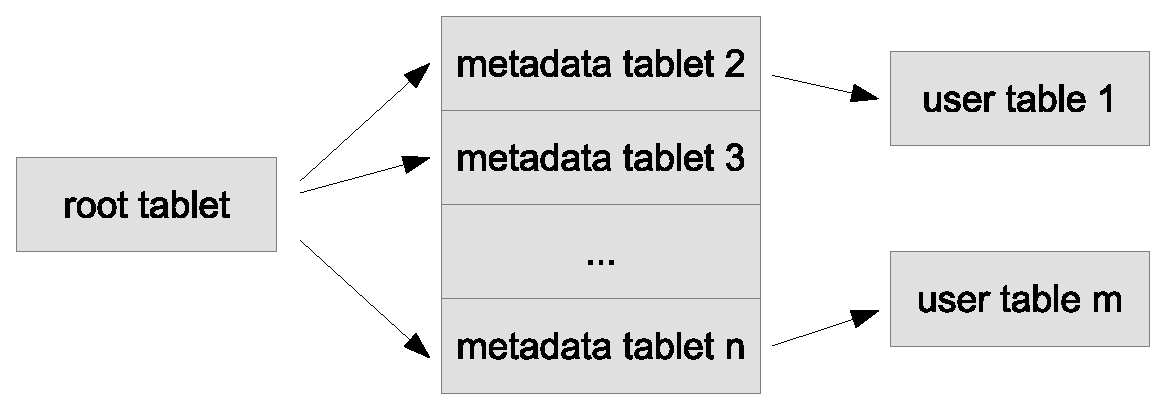
\includegraphics [width=0.7\textwidth]{images/bigtable_tablets_hierarchy}
  \caption{Bigtable tablets hierarchy}
  \label{fig:bigtable_tablets_hierarchy}
\end{figure}

\mnote{SSTable}
Bigtable stores data in special file format called SSTable.
Each SSTable consists of several blocks of a fixed size (64Kb by default). 
To locate blocks it stores their indexes, that are loaded into memory on opening the SSTable.
The blocks indexes considerably decrease the lookup time.
First the binary search is performed on in-memory index to find the needed block.
Than the appropriate block is read from disk.
The whole SSTable can be loaded into memory if necessary to perform lookup and scan operations avoiding touching disk.

A tablet can be recovered using a commit log.
This log contains all the tablet updates.
The most recent updates can be obtained from a memtable - a sorted buffer in memory.
The set of SSTables stores the older updates. 
A tablet server can read the METADATA table to detect the necessary SSTables for recovering.
Than the tablet server applies all the updates in order to restore the crashed tablet. 
  
A tablet server checks the incoming read and write operations.
The operation should be well-formed and the sender should be authorized to perform a mutation.
First the server writes a valid mutation to the commit log.
Then for write operation it inserts its content to memtable.
When the size of the memtable goes beyond the given threshold, the system frozes it.
It creates a new memtable and converts the frozen one into an SSTable. 
Read operation is performed on a merged view of the memtable and corresponding SSTables.

Periodically a merging compaction on SSTables and the memtable are used to create new SSTables out of old ones.
A regular compaction merges the memtable and a few SSTables, keeping the deletion information and deleted data.
A major compaction merges all SSTables into exactly one SSTable, cleaning deletion entries.
Bigtable performes the compaction mechanism regularly to keep the system up-to-date.

The variable number of tablets makes the system flexible and therefore easy to scale.
The implementation features provide good performance and high availability.
Bigtable is successfully used in many Google products, that proves the high quality of this storage system.

% Other BigData systems:
%Malewicz - Pregel
%Melnik - Dremel
%Akidau - MillWheel

\section{Facebook Architecture}

Facebook is another representative company that is strongly connected with Big Data storing and processing.
The main difference is that Facebook applications often require real-time data processing, providing a user with immediate feedback.
On the contrary, for most Google applications batch processing is sufficient to make necessary computations.

\mnote{Facebook architecture}
Figure~\ref{fig:facebook_data_flow} demonstrates the data flow in Facebook architecture.
Data originates from two sources: web servers and federated MySQL instances.
Web servers generate log data, that consists of variuos events, e.g. a user clicked a link or 'liked' a photo.
The federated MySQL contains the descripting data, such as the time of posting the link and the place where it was done.

\begin{figure}
  \centering
  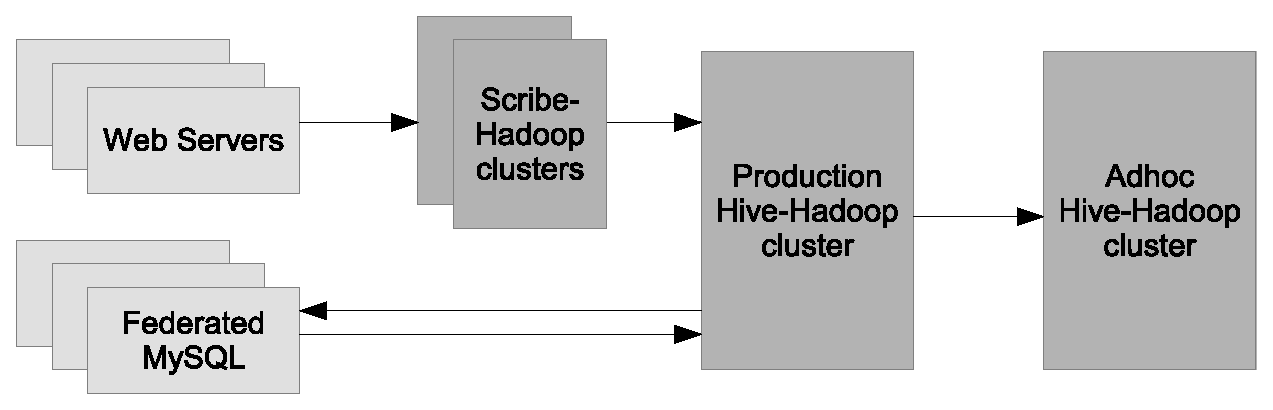
\includegraphics [width=0.9\textwidth]{images/facebook_data_flow}
  \caption{Data flow in Facebook}
  \label{fig:facebook_data_flow}
\end{figure}

Data flow goes from web servers to Scribe-Hadoop clusters.
Such cluster is actually a Hadoop cluster with a running Scribe server on the top of it.
The main function of Scribe is to aggregate the input data and write it into HDFS.
This data is transferred uncompressed [Data Warehousing and Analytics Infrastructure at Facebook] that can be a bottleneck for the whole system.
Facebook alleviates the problem by putting Scribe-Hadoop close to web servers, decreasing the network transfer load.
Periodically Scribe-Hadoop clusters send compressed data (mostly as HDFS files) to Hive-Hadoop clusters.
It is loaded to Hive and becomes available for other modules.

Scrape processes load data from federated MySQL to Hive-Hadoop cluster.
They get a dump of needed data from database, compress it and move it to the cluster.
This process should be resilient and avoid putting extra load on the databases.
The former is accomplished by using the previous days data when the database is not reachable at the moment.
To meet the latter requirement, scrape process runs on a MySQL database replica.

There are two types of Hive-Hadoop clusters - a production cluster and an adhoc one.
The purpose of the production cluster is to execute high prioriy tasks with strict deadlines.
On the contrary, the ad hoc cluster processes batch jobs with low priority and makes ad hoc analysis.
These tasks are separated, because it can be dangerous to run ad hoc user query on a production cluster.

When the data is needed for both clusters, it is replicated from the production to the adhoc cluster.
It is done in this order, because the data should be available earlier for critical jobs on the production server.
Moreover, the production server is more reliable.
During the replication process the data is transferred in a raw form accompaned by the respective metadata.

The stored data can be either transformed or queried by users.
Most of the time Hive-Hadoop clusters keep the data for future analysis.
However, in some cases the federal MySQL tier gets the data back.
This data can be uploaded on the Facebook site and participate in the further interaction with Facebook users. 

The amount of data stored on a Hive-Hadoop server is huge.
That is why Facebook compresses it using gzip.
Moreover, a special row columnar compression is used to store data in Hive.
Also Facebook uses erasure codes to provide fault tolerance and at the same time decrease the amount of data copies stored on different machines.
Erasure coding is a technique when the messages of length \textit{n} are transformed into the longer messages of length \textit{m}.
This expanded data is spread across several locations.
Later on it is possible to recover the original message using only a subset of \textit{m} symbols.

Facebook widely uses such technologies for distributed data warehousing and computation as HDFS, Hive and Scribe. 
While HDFS is an exterior module, Hive and Scribe were initially developed at Facebook and only later became open-source under the Apache Software Foundation.
HDFS is described in detail in Chapter 7 (Components), Hive and Scribe are presented in the following sections.

\mnote{Hive}
Hive is a framework designed for storing data.
Facebook uses it to query and analyze data.
Hive provides an SQL-like interface for accessing the data from Hadoop.
This makes the process of development easier comparing with a direct interaction with Hadoop via map-reduce.

Figure~\ref{fig:hive} presents the Hive structure.
Hive has a \textit{Metastore} that stores mappings between Hive and Hadoop.
The \textit{Driver} communicates with the Metastore and uses the obtained information for converting Hive query language (HiveQL) expressions into map-reduce jobs.
Hive provides various types of interfaces for interaction: web based Graphiclal User Interface (GUI), a command line, Open Database Connectivity (ODBC), Java Database Connectivity (JDBC).
The latter two communicate with the Driver using Thrift server, that represents a communication protocol for performing remote procedure calls in numerous programming languages.

\begin{figure}
  \centering
  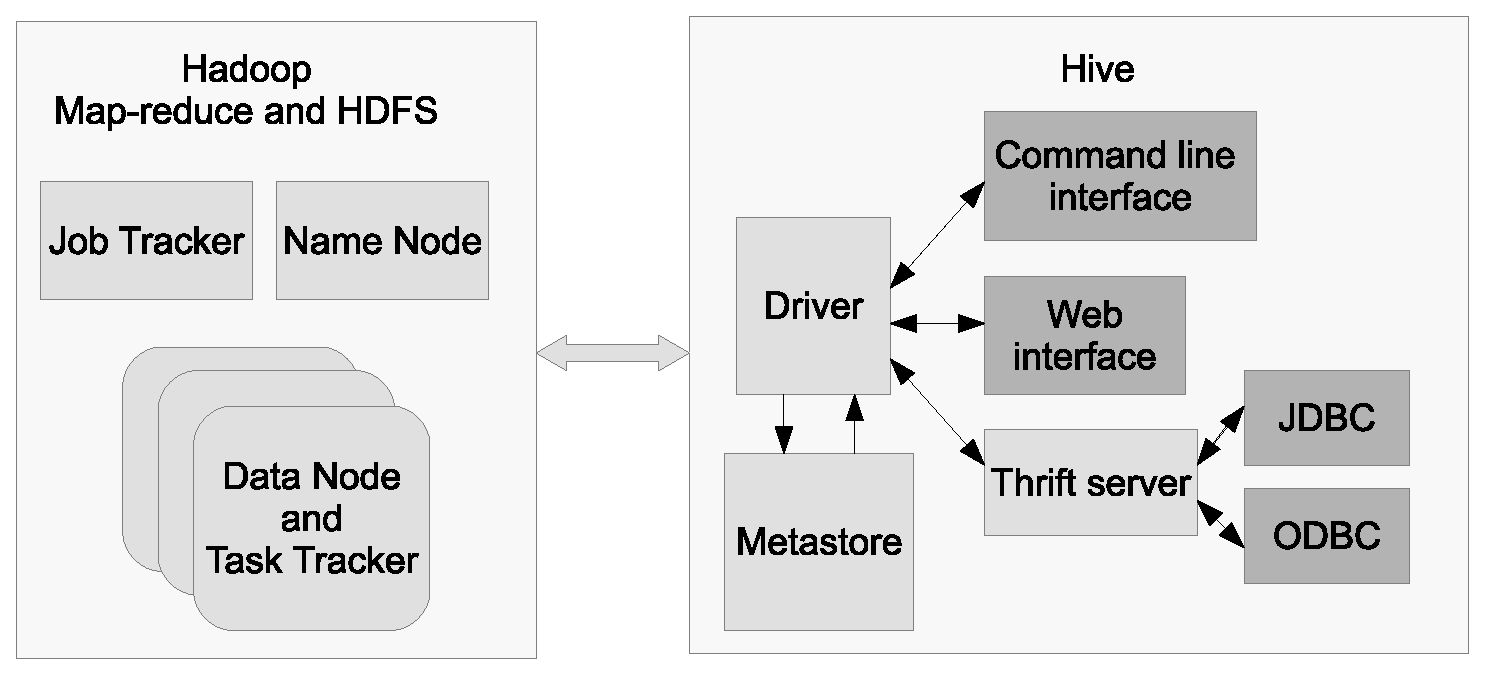
\includegraphics [width=0.9\textwidth]{images/Hive}
  \caption{Hive structure}
  \label{fig:hive}
\end{figure}

The Driver applies several types of optimization during the compilation process.
First, it uses file pruning and filtering to reduce the amount of data that should go to map-reduce jobs.
Then it uses column pruning to exclude columns that are not needed for the query.
Also the Driver uses such aggregations as 'group by' or 'join' for optimization.
Join techniques vary in the effect they have on the way of processing data.
For instance, reordering join allows to stream large tables to a reduce task avoiding helding it in memory.

Hive is a flexible framework and can be customized for the user needs.
A user can define functions, table functions or scripts written in HiveQL.
Moreover, it is possible to define custom types and data formats.

\mnote{Scribe}
Scribe is a distributed logging system designed for logging huge amounts of data. %[https://github.com/facebookarchive/scribe/wiki]
It can be spread to thousands of nodes.
At the same time it guarantees fail tolerance in the case of network or node crashes.

There are two types of servers in Scribe: general servers and central servers.
They are connected by a directed graph.%[https://www.facebook.com/note.php?note_id=32008268919]
In this graph each node knows only the next node and is not aware about the others.
This makes the communication easier, because it saves the sender from the necessity to know the network topology.

The servers interact via messages.
The data model of Scribe is simple, without timestamping, message ordering, logging levels, etc.
A message in Scribe consists of two strings: a category and a message itself.
A category reflects the message topic.
It is implied that the messages in one category have the same destination.
Categories allows to move a data store without changing a client code.
For this purpose Scribe uses the server configuration settings.
Moreover, the server can be configured to put into the file path a category name.
The message string contains the information that should be logged.

Scribe provides fault tolerance in the case of a network or machine failure as follows.
The servers send messages to the central server/servers.
Central servers, in their turn, write messages to the final destination, such as Network File System (NFS) or distributed filesystem.
When the server cannot send a message to the central server because of the network problems or the central server crash, it stores this message locally.
With random time intervals it tries to reestablish the lost connection.
To prevent the central server overload when it recovers after the failure, it can reply with the TRY LATER message.
In this case the receiver must wait several minutes before the next attempt.
The central server follows the same logic when it cannot connect to the distributed filesystem or NFS. 

However, there are some scenarios that can lead to the data loss.
For example, when the server or the central server is not available from the client side.
Or in the case of the central server crash it loses the information that was not written on disk and was kept in memory at that moment.
Or when the local disk capacity is exceeded while the central server is not available.

Scribe is based on Thrift, a software stack designed for code generation for RPC in multi-language environment.
It allows to use different languages like PHP, C++, Java or python for working with it.
The detailed discussion about Thrift is presented in Chapter 7 (Components). 
Thrift reach functionality solves many hard problems connected with logging, extending Scribe capabilities.

Scribe configuration files specify which store should be a destination for a particular directory.
There are various types of stores.
Some of them consists of other stores, like a batch store, that is build of a number of file stores.
The configuration file has a section for every store along with a global section.
Such setting as the maximum message number per second or the listening port are stored in the global section.
All the store sections contains information about a type and a category.
The number of categories is not limited as well as the number of stores for one category.
Also the store section can include specific settings that are needed for a particular store type, like maximum size of a file or its location.

\mnote{Databee}
Facebook uses Databee for managing job dependencies.
Databee is a framework written in python.
Its aim is to make the interaction process between parts of the system easier.
For example, it transmitts data from one part of the system to another, transforms data and allows to run queries on it.
Also Databee creates monitoring information, that contains such details as job latency or job completion time.
It allows to specify dependency on some data set.
Thus it is possible to run a job at the time when a needed data set becomes available.

As Facebook supports both ad hoc and periodic batch jobs, it needs a proper mechanism for sharing resources.
Periodic jobs, in contrast to ad hoc ones, have strict deadlines.
At the same time, it can happen that a long running periodic batch job blocks a short ad hoc query, holding the resources.
For the purpose of the proper sharing Facebook introduces Hadoop Fair Share Scheduler.
It divides users into pools and each of these pools are provided by the same quota of resources.
This scheduler limits the amount of concurrent jobs running in one pool.
The periodic batch jobs have their own pools.
It is guaranteed that even in the case of high load these pools are provided at least a minimum quota of resources.
Hadoop Fair Share Scheduler keeps track of the CPU and memory consumption by every node in a cluster.
The scheduler is able to kill a job that consumes memory more than allowed threshold.

\mnote{HDFS in Facebook}
[Apache Hadoop Goes Realtime at Facebook]
In matters of warehousing Facebook relies on HDFS.
This file system provides a reliable, extensible and highly available store.
However, for use cases, specific for Facebook, it has a significant disadvantage.
It is designed for batch processing, while Facebook needs a system that can handle data in real time.
Therefore a number of enhancements were introduced to make HDFS more suitable for the existent requirements.

HDFS has a node called NameNode, that serves as a master node for the cluster.
To prevent NameNode being a single point of failure, HDFS uses a BackupNode.
In the case of failure the schema works as follows.
First, a NameNode reads a metadata file, recreating a file system image.
Second, a NameNode waits for the replies from DataNodes, that should report about their location.
The presence of the BackupNode helps to avoid the first step.
The BackupNode stores the copy of the file system image.
Nevertheless, the second step is still necessary and takes considerable time to complete.

To make the cold-start process fast, Facebook introduces an AvatarNode.
There are two AvatarNodes in a cluster.
One of them is an Active AvatarNode, that represents a wrapper around a NameNode.
The second one is a hot-standby copy of the former.

Figure~\ref{fig:facebook_avatarnode}  illustrates how two AvatarNodes interact with each other.
The Active AvatarNode stores a filesystem image and a transaction log in a Network file system (NFS).
Simultaneously the Standby node reads this information and applies all the transactions.
DataNodes send the location information to both Active and Standby node.
Thus the Standby node can replace the Active one at any moment.
Facebook also modified the transactions form, enriching it with id, data length and a checksum.
This helps to avoid reading a partial transaction by the Standby AvatarNode.

\begin{figure}
  \centering
  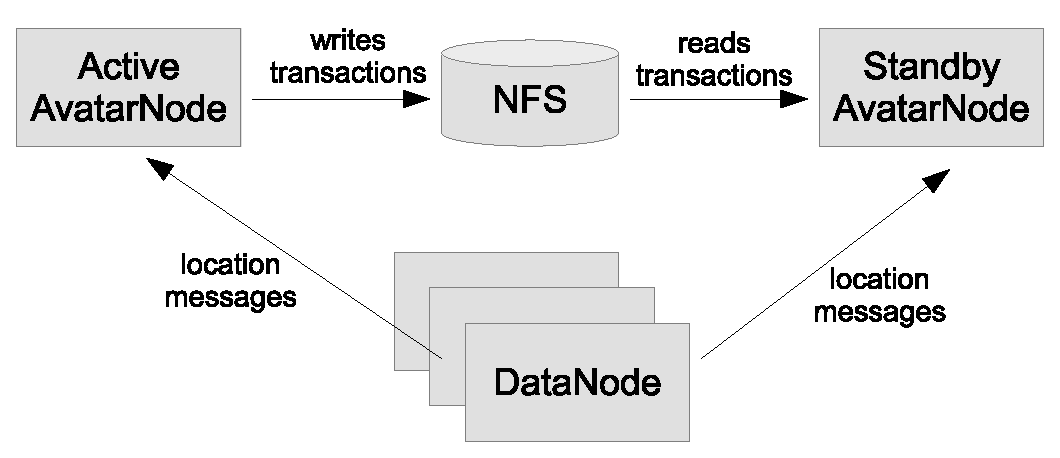
\includegraphics [width=0.7\textwidth]{images/facebook_avatarnode}
  \caption{AvatarNodes interaction}
  \label{fig:facebook_avatarnode}
\end{figure}

Facebook has improved an RPC mechanism.
As the company controls the huge number of machines, it should be able to cope with a situation when different clusters have different Hadoop version installed.
Therefore the implementation of RPC was changed.
It became possible to detect the Hadoop version automatically and use the appropriate protocol for communication.
Also Facebook added a possibility to specify an RPC timeout.
Originally, Hadoop was designed in such a way that the client is waiting for the reply from an RPC server infinitely.
However this is inadmissible for real-time applications.

HDFS was extended by \textit{recoverLease} API, that significantly decreases the lease revokation time.
Before this enhancement HDFS used a soft lease mechanism.
In this case, when the clien cannot read the file, it continues read tries until success or until the soft lease expires (that was one minute by default).
Due to the \textit{recoverLease} it becomes possible to revoke a lease immediately.
A \textit{recoverLease} request is received by the NameNode.
At that moment it becomes a holder of the file and starts to recover the lease.
When it is done, the NameNode replies with 'recovery complete' message.
Then the client can start reading from the file.

\mnote{HBase}
Facebook uses HBase as a database. 
HBase is a distributed database that is built on a basis of BigTable and runs on top of HDFS.%[http://hbase.apache.org/book/architecture.html]
HBase can be called as one of the implementations of BigTable, therefore it has an identical structure.

Facebook optimizes the database for its own needs.
For example, to improve write performance, the following steps are applied.
First, data is stored into a commit log.
Then it goes to Memstore, an in-memory cache.
Memstore gathers data until it reaches a limit and then write it as an HFile to HDFS.
HFile is a file format for HBase, that contains a sorted set of key-value pairs.
With every flush operation a new HFile is created.
Thus these files should be merged periodically for better read performance.
This process is called files compaction.

\mnote{Haystack}
Haystack is another technology used by Facebook to solve problems of large-scale data.
It is an object storage system designed for working with billions of files.%[Finding a needle in Haystack: Facebook�s photo storage]
Facebook uses it for photo warehousing.

Photo storing differs from other storage system applications.
The storage system writes a photo only once and never modifies.
Also photos are read quite often.
Photos do not need most of the metadata information usually stored by a file system for each file.
Moreover, Facebook requires a fast way to find and read a photo.

Haystack is specifically designed to meet all the Facebook requirements.
Figure~\ref{fig:haystack_architecture} shows the Haystack architecture.
The main three parts of Haystack are Haystack Directory, Haystack Store and Haystack Cache.
The Store contains photos and associated metadata.
The Store is devided into logical volumes, each of them combines several physical volumes.
The Directory is responsible for mapping between logical and physical volumes.
The Cache is a content delivery network (CDN), that provides access for most frequently asked photos.

\begin{figure}
  \centering
  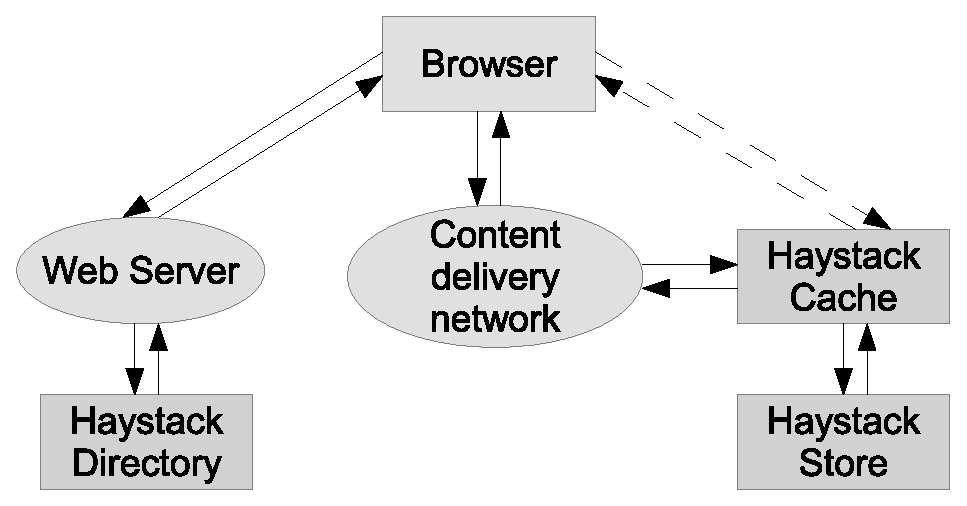
\includegraphics [width=0.5\textwidth]{images/haystack_architecture}
  \caption{Haystack architecture}
  \label{fig:haystack_architecture}
\end{figure}

The typical scenario of a user-Haystack interaction can be described as follows.

1. The user visits a page that contains some photos.

2. The web server receives a request from the browser and asks the Directory for the photo URL.
The URL has the following structure: http://[CDN]/[Cache]/[Machine id]/[Logical volume, Photo id] %[Finding a needle in Haystack: Facebook�s photo storage]

3. The browser communicates with the CDN specified in the URL. 
In some scenarios the browser communicates directly with the Cache, passing over the CDN.

4. The CDN searches for the photo locally, using the Logical volume and Photo id information.

5. If the photo is not found, the CDN transfers the request to the Cache.

6. The Cache performs the same actions and if the photo is still not found, it asks the Store machine.

When the user uploads a photo:

1. The web server askes the Directory for the logical volume where the photo can be written.

2. Then the server assignes an id to this photo.

3. Finally it saves the photo on every physical volume assiciated with the given logical module. 
 
\mnote{Haystack Directory}
The Directory has four main applications in Haystack.
First, as it was mentioned, the Directory manages a mapping between logical and physical volumes.
Second, it performs the load balancing.
The Directory controls the write and read load among logical and physical volumes correspondingly.
Third, it determines read-only logical volumes.
A logical volume becomes read-only, for example, when it does not have free memory for storing new photos.
Forth, the Directory specifies which component (CDN or Cache) should be used by the browser.    

\mnote{Haystack Cache}
The Cache is a distributed hash table.
Haystack uses a photo id as a key to obtain the needed photo.
The Cache stores the photo only when it receives a request directly from a browser, not from the CDN.
Also it is necessary that the photo is located on a write-enabled machine.

\mnote{Haystack Store}
Every Store machine contains several physical volumes.
One such volume can be considered as a very large file, containing millions of photos.
This is done to decrease the amount of metadata stored for each file.
To obtain the photo, the Store needs a logical volume id and the file offset.
The Store keeps in memory the mapping between the photo id and its offset, size and other metadata information.
This allows to make the process of photo retrieving fast.

A physical volume consists of a sequence of needles, where one needle is associated with one photo.
Each needle contains: a Header with information for recovery, a Cookie to prevent brute force lookups, a Key and an Alternative key, Flags showing deletion status, a Size, the Data itself, a Footer also used for recovery, a Checksum and a Padding.
The Key is represented by the photo id and the alterative key by its type.
The type in this case denotes the size - each photo on upload is scaled to four different sizes.
The cookie is a number randomly assigned by the Directory.
It is added to the photo URL and prevents attacks for guessing the URL.

There are three actions that the Store can perform with a photo.
First, the photo can be written.
A Cache machine sends a request to Store machines, containing a key, an alternative key, a logical volume id, a cookie and the data to be stored.
Every store machine saves the data and updates mapping that are stored in memory.
The Store supports only append operation, so the data once written cannot be modified.
Thus when a new version of a photo should be stored, the Store adds an updated niddle that has the same key and alternative key.
Different versions are distinguished by different offsets in a file.

Second, the Store allows to read photos.
A Cache machine sends the same data as with writing, except the data to be stored.
The store searches for the necessary metadata in memory.
The Store finds the necessary file and seeks for the specified offset in it.
It reads the appropriate needle.
Finally some verifications like cookie check or data integrity are performed. 

Third, a photo can be deleted.
When the photo is deleted, the Store sets two flags: one for in-memory mapping and one for the volume file.
If the Store receives a request for a deleted photo, and the in-memory flag is set to 'deleted', the Store returns an error.
Deleted needles still occupy the space on disk, so it is released using the file compaction.

Haystack uses an \textit{index file} for optimizing the time of Store machines reboot.
The problem is that every machine has to restore its in-memory mappings.
Instead of inspecting all its physical volumes on reboot, a Store machine reads the index file.
The index file has the similar structure to physical volume files.
It contains a set of records, where one record corresponds to one needle.
It is important that the ordering of records should be the same as the ordering of needles.
The index file has the following fields: Key and Alternate key, Flags, Offset and Size.

When a photo is written into the Store, the index file is updated asynchronously.
When a user deletes a photo, the index file is not changed at all.
This is done to improve the performance.
However, it brings some problems: (1) it is possible to have a needle without a related index record, (2) index file has no information about deleted photos.
The needle that has no record in index file is called an \textit{orphan}.
The Store machine gets rid of orphans during the reboot process: for each orphan needle it creates a record in the index file.
To solve the second problem, the Store checks the deleted flag on receiving a read request.

Haystack uses a background task called \textit{pitchfork} to recover from failures.
This task is responsible for checking the state of all the Store machines peroidically.
It should check the connection, volume files availability and the ability to read data.
If the tests are failed, all the logical volumes of this machine are marked as read-only.
Then such machines are manually examined to find the reason of failure.    

 







% 1. Flow of data (Data Warehousing and Analytics Infrastructure at Facebook)
% 2. HDFS enhancement + HBase + Hive + Scribe (Data Warehousing and Analytics Infrastructure at Facebook) + (Apache Hadoop Goes Realtime at Facebook)
% 3. Haystack (https://www.facebook.com/note.php?note_id=76191543919) + (Finding a needle in Haystack: Facebook�s photo storage)
% 4. jemalloc (https://www.facebook.com/notes/facebook-engineering/scalable-memory-allocation-using-jemalloc/480222803919)
\chapter{Real time processing in the Big Data context [VI]}
\label{chap:real_time_processing}

\section{Something about Twitter}

\section{Bloom filter, other algorithms}

\section{Kafka paper}

\section{Speed Layer (for real time processing)}
\chapter{The Lambda Architecture [VI]}
\label{chap:lambda_architecture}

%New terms:
% view
% batch layer
% batch view
% serving layer
% speed layer
% real-time view
% raw data
% immutability

The Lambda architecture is a new solution for generic BigData systems \cite{MarzWarren201401}.
To answer queries it uses both batch and online processing.
It fulfills all requirements that such systems demand, e.g. scalability, extensibility, fault-tolerance, etc.
It provides human fault-tolerance, what is often overlooked in other approaches.
All its components automatically distribute computations across many machines.

%The core purpose of the Lambda architecture is to answer queries, having data, gathered during system's functioning.
%We consider any query as a function of the whole dataset, i.e. taking all available data, system can derive information, that answers specific query.
%The Lambda architecture is also able to answer queries that have not yet arised to the moment of the system's design or deployment.

The Lambda architecture uses both batch and online processing of data to answer queries fast as well as accurate.
It applies batch processing to all data to precompute specific data structures helping to answer queries with low-latency.
It also executes online incremental processing of arriving data, what helps to overcome delay of batch computations.

The Lambda architecture has all properties to be an effective and efficient BigData system.
It is robust and fault-tolerant.
It provides low-latency query answering.
It is scalable, generic and extensible.
It allows to make ad hoc queries, requires minimal maintenance, and is debuggable.

Important aspect of the Lambda architecture, that makes a difference with other approaches, is that human fault-tolerance is inherent.
Human fault-tolerance is a robustness of the system to mistakes in programming code.
This is important issue, because programmers always do mistakes.
As a result, deleting or updating the data in a wrong way is also possible.
The Lambda architecture overcome this issue not allowing to delete or modify so far gathered data.

The Lambda architecture is a distributed system.
Every its part provides this property inherently.
That lets developer to concentrate on the logik and algorithms, instead of thinking about multithreading issues.

\section{General structure}

%System must provide information having gathered data from users and other sources.
%Application of complex algorithms is often necessary.
%Amount of data and rate of its arrival are heavy.
%Those aspects makes system to preprocess indices and aggregations that provide useful information.
%Batch processing is a good solution for that, nevertheless it has drawback - execution time is long.
%Incrementall processing resolves this issue.
%In combination these two approaches allow to design a system, that answers user queries with low latency as well as accurate.

%The purpose of the system is to answer queries having data.
%Let's consider an artificial example.
%Suppose we have a website where people pose programming questions, and other answer them.
%In this case the simplest query to the system is to return list of answers for a particular question post.
%Another query is to find all posts containing given keyword.

%One query is easy to answer, another requires application of complex algorithms.
%It is pretty easy to get list of answers to the question post having its id.
%You simply create hash-table that maps questions' ids to lists of answers' ids.
%Search by keyword, or even phrase search, is much more complex.
%To make it possibe we have to build specific inverted index, and this requires much more time to execute and to programm.
%Let's further assume, that our system has to provide keyword search, using precomputed inverted index. 

%Amount of data gathered with the time, as well as intense of arrival, can be huge.
%Let's consider again our example website.
%Assume that on average every second 5 questions and 20 answers appear.
%Every post is about 100 words, each of about 8 unicode symbols.
%The rate of incoming data is then $25*100*8*2=39$ KB per second.
%It is about 3.2 GB per day.
%This leads our system to be able to process such amount of data efficiently, as well as to rapidly reflect the state of inverted index with newly arrived posts.

Amount of data and complexity of algorithms demand to make computations, useful for fast answering queries, in advance.
The Lambda architecture precomputes specific data structures, that provide data, prepared as much as possible to directly answer specific queries.
We call these data structures \textit{views}\mnote{view}.
They store indices and aggregations of original data.
%In our example we consider inverted index as a view.
%In a query time it provides efficient search of all posts with particular keyword.

There two approaches of preparing views.
The first one is to do it in a batch mode considering all available data for computations.
The second one is to construct views incrementally in the real-time with newly arrived data.
Together these two methods give us an opportunity to answer queries fast and accurate.
Figure~\ref{fig:lambda_architecture} depicts how the Lambda architecture combines batch and incremental processing to answer queries.

The \textit{batch layer} \mnote{batch layer} of the Lambda architecture is responsible for batch processing.
It takes the whole dataset and executes batch computations on it.
Views, that are the result of the batch processing, we call \textit{batch views} \mnote{batch view}. 
This operation is efficient, because all data is at once in disposal.
We can execute any algorithm, and produce any kind of index or aggregation.
It is also easy to programm using such greate batch processing approaches as MapReduce.
This paradighm is inherently distributed and scalable.
%In example with website we would use MapReduce to create inverted index having all posts.
%It requires only several lines of code in the simplest case. 

\begin{figure}
  \centering
  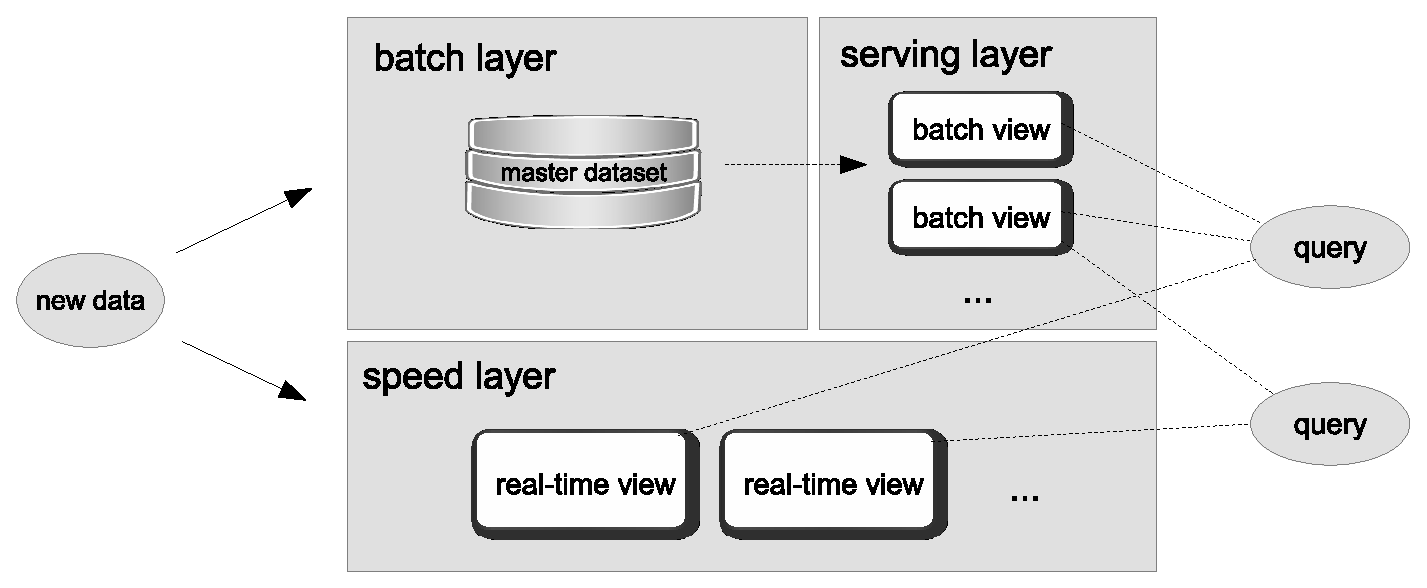
\includegraphics [width=1.0\textwidth]{images/LambdaArchitecture}
  \caption{General structure of the Lambda architecture. Batch and sevring layer are responsible for batch views, speed layer provides real-time views. To answer query system merges data from both types of views.}
  \label{fig:lambda_architecture}
\end{figure}

After the batch layer has precomputed views, it places them into the \textit{serving layer}\mnote{serving layer}.
The serving layer is responsible for storage of batch views.
It also creates indices on those views and provides interfaces to get particular data records from them.

Batch layer starts then computations again, considering now data, that has come during the last batch processing.
This loop goes on infinitely.
Batch processing always starts again from scratch using all available data.
When the batch layer stores computed views into the serving layer, it discards old ones.

Batch computations, although easy and efficient, take long time to be done.
This cannot be underestimated, because on the BigData scale computations can last hours even if we setup cluster of thousends of machines.
%In website example, assume our system has already been working for a year.
%It has then about 800 millions of posts.
%If we have a cluster of 100 machines, each has then to perform map-function 8 millions times.
%If one execution of map-function takes 1 milisecond, it leads to 2.2 hours of total computations.
%And we have not even counted reduce-phase.

As long as batch computations take much time, views are always outdated for several hours.
During this time new data arrives to the system, and it must be also counted in query answers.
This is not possible to solve using only batch processing.
Therefore, another approach is to apply.

To overcome delay of batch computations the Lambda architecture has additional component - the \textit{speed layer}\mnote{speed layer}.
It also computes views, but in incremental fashion.
We call them \textit{real-time views} \mnote{real-time view}.
As new data arrives, the speed layer updates incrementally real-time views.
Hence, they always has information from data, gathered during current batch processing.

Finally, to answer queries system uses both batch and real-time views.
Batch views contain result of the last batch processing.
Real-time views provide infromation from data, gathered after the beginning of the current batch processing.
Merging both types of views, system produces accurate and actual answers to the queries.
\section{Batch Layer}

The batch layer is the heart of the Lambda architecture.
It is the place where all ever gathered data resides and being processed.
The batch layer executes two main tasks: storing of data arriving from outer sources, and processing of that data to create batch views, used for the low-latency query answering.
The first issue requires usage of a storage system that provides fast appending, efficient batch reads, and no random reads/writes of data.
Computation of batch views demands application of distributed efficient batch processing algorithms as for example MapReduce.

\subsection{Data Model}

The batch layer requires usage of a specific data model to make the Lambda architecture scalable, highly efficient and fault-tolerant.
This data model is based upon four main notions.
\textit{Information} - the whole knowledge, that system holds.
\textit{Data} - collecting notion for records, strings, values, etc., kept in the system, so that they cannot be derived from any other data.
\textit{Query} - a question that is asked to the system, and demands a piece of information that answers it.
\textit{View} - a data structure that holds information directly useful for answering query.

\mnote{Raw data}
To answer as much different queries as possible, the batch layer stores only \textit{raw data}.
It is possible to derive from it data, particularly relevant for query, but not vice versa.
This is important, because the system does not know in advance all queries it will have to answer in the feature.
The more basic is the data, the more information can be possibly deduced from it.

In the current context, unstructured data is always better than normalized, because it is rawer.
As an example, let us consider the system, that stores users' search of a geographic location.
Suppose that system stores all those queries for further analytics.
If it saves them normalized, or in other words parsed and mapped to a known geographic location, it can for certain queries save nothing or NULL value, because algorithm cannot execute correct mapping.
In other case, when the system stores raw string, that user typed, it can later on have this data properly parsed, if parsing and mapping algorithms are improved.
This example shows, that unstructured raw data is preferred to store in the batch layer.

\mnote{Data immutability}
The batch layer does not allow modification or deletion of data, what is called \textit{immutability}.
It only allows appending new records.
This property gives two crucial advantages.
Immutability dramatically simplifies complexity of the storage mechanisms.
This is because maintenance of modifications in the distributed environment is not an easy task.
To successfully update a record, the system must perform it for all replications, provide locks and prohibit simultaneous updates.
It has to maintain versions of the same record for different users.
Absence of all these and many other requirements saves from much of complexity.
The system is easier to understand, repair and improve.
It is much safer from programming mistakes and consequent errors.

\mnote{Human fault-tolerance}
Another advantage of immutability is that mistakes in algorithms cannot corrupt data anymore.
This property is called \textit{human fault-tolerance}, and it is very important, because programmers always do mistakes.
As a result, it is possible, that wrong code can incorrectly update or delete data.
When data is immutable, programmers' mistakes can only append wrong data to the dataset.
This can be later repaired by administrator, but all proper data is always safe.

Immutability leads to high growth of data volume, because everything last stored basically forever.
This is, however, not a problem, because, as we discuss later on in this chapter, the batch layer is purely distributed and scalable.
It allows increasing capacity of its data store to any extent, adding new machines at any time.

Immutability requires completely different data model, comparing to relational databases, that manipulate tuples of complex objects altogether.
In contrast, the batch layer stores each attribute of a logical tuple separately.
Each value has the timestamp of addition moment. 
Such technique allows having the whole history of logical updates of all records.
The actual value is the one with the oldest timestamp.

\mnote{Eternal truthfulness of data}
Immutability gives one more important property of data, stored in the batch layer, namely \textit{eternal truthfulness of data}.
When new record is added, no matter is it a new piece of data or update of an old data, it represents true information in that particular moment in time.
This never becomes false, because it describes event or state of the world that is an occurred fact.
This property implies that the batch layer not only stores data, describing the state of the system, but also the history of its state changes.

\mnote{Master dataset}
Having defined the main properties of data, we can introduce the notion of the \textit{master dataset}.
The master dataset is the main storage, where all the data that ever arrived to the system resides.
The batch layer is responsible for its maintenance.
If there is a fault of the master dataset - all data can be lost.
And data is of the most importance in this context.
Therefore, the master dataset must be carefully designed, set up and protected.
It must be saved from all types of failures, e.g. software, hardware or human.
The master dataset is logically a large list of records.
When new piece of data arrives into the system, the batch layer appends it to the master dataset.
The more exact description of how the master dataset can look like will be discussed later on in this chapter.

\begin{figure}[h]
  \centering
  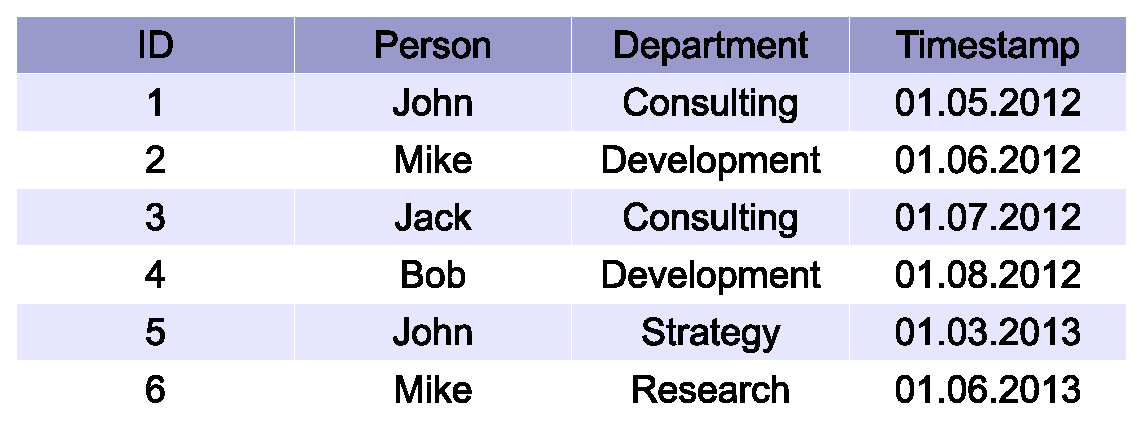
\includegraphics [width=0.8\textwidth]{images/MasterDatasetExample}
  \caption{An example of the list of records in the master dataset.}
  \label{fig:MasterDatasetExample}
\end{figure}

On the Figure~\ref{fig:MasterDatasetExample} there is an example of the list of records of the master dataset.
The 5th and 6th records are updates of the 1st and 2nd, respectively.
They are in the same list, but the current version is defined by the last timestamp.
This model implies, that the whole history of updates is available at any time in the future. 

\mnote{Fact-based model}
In contrast to relational databases, data in the master dataset is stored using a so called \textit{fact-based model}.
It supposes that all the data is divided into simple units called facts.
Fact has several properties.
It is timestamped on addition to the master dataset.
Fact cannot be divided to a smaller units, it is already atomic.
Fact is identifiable in the sense that any two facts in the dataset must be distinguishable.

Fact-based model offers several important advantages.
It allows to make queries to a state of the dataset at any time in its history, because each piece of data (fact) is timestamped and immutable, or, in other words, eternally true.
It provides human-fault tolerance, as long as facts are immutable, and if a fact is added mistakenly, administrator can delete it.
If any of attributes of a complex object are absent, it is not necessary to store any NULL values, because data is stored in atomic facts.
Data can be stored in an unstructured denormalized form, because it is not queried directly from the master dataset, but from batch views of the serving layer, discussed later on.

\mnote{Graph schema}
To unite facts into related data there are so called \textit{graph schemas}.
Graph schema is a graph that describes the structure of a fact-based model.
It defines relations between entities similarly as entity-relationship model does for relational databases.
Graph schema consists of three elements: nodes, edges and properties.
Nodes are entities representing particular objects of a describable system.
Edges define relationships that connect nodes into the specific structure.
Properties provide information associated with nodes.

\begin{figure}[h]
  \centering
  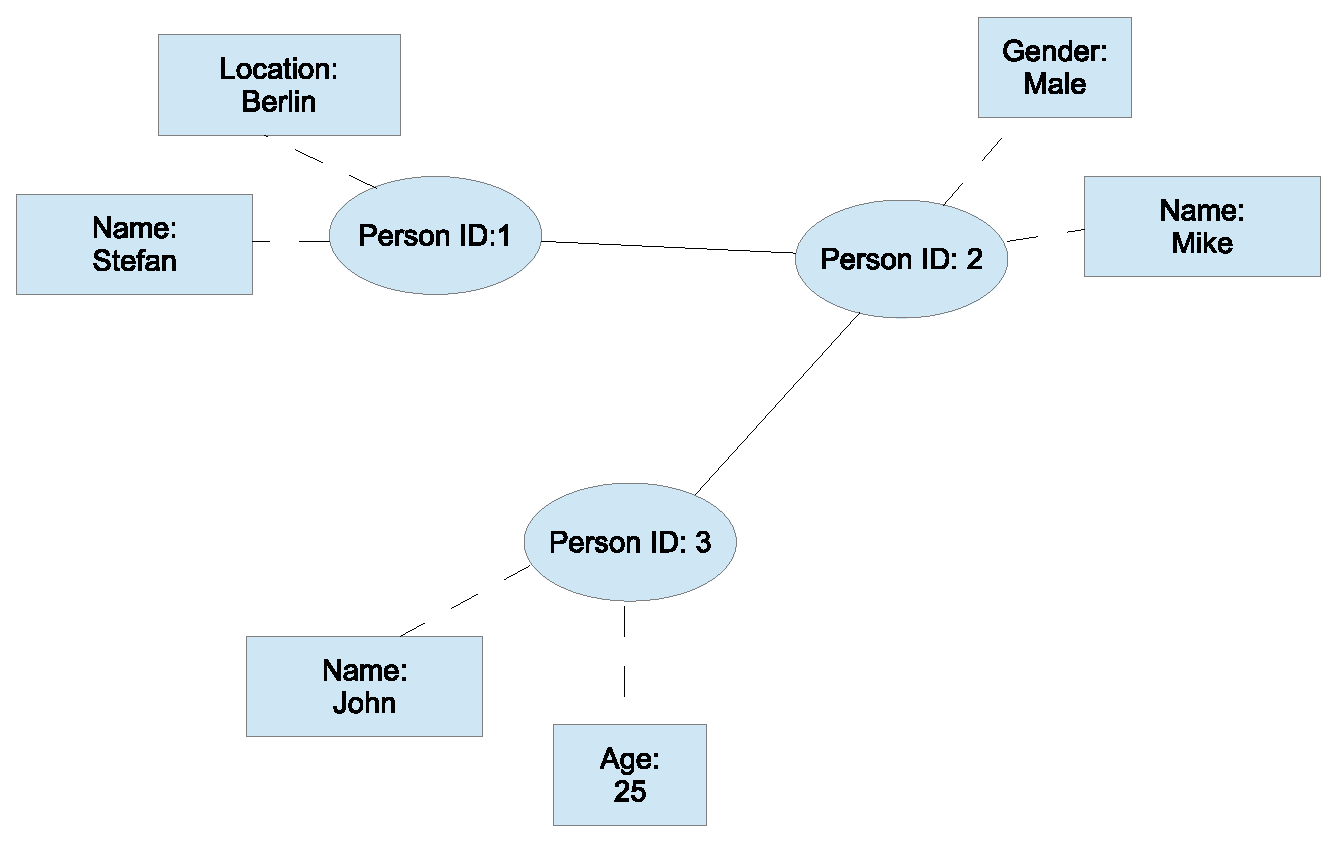
\includegraphics [width=0.8\textwidth]{images/GraphSchema}
  \caption{An example of graph schema.}
  \label{fig:GraphSchema}
\end{figure}

Figure~\ref{fig:GraphSchema} shows an example of a graph schema for a simple data model.
Entities are represented using ovals.
They are persons in this case.
Users are connected with their properties via dashed lines.
Lines between entities are edges.

\mnote{Serialization frameworks}
To save developers from detailed implementation of graph schema every time, and from possibility to do mistakes during this process, there are so called \textit{serialization frameworks}.
They provide a useful tool that generates all needed code, having described schema of the dataset in a specific descriptive language.
Serialization frameworks require only description of key notions, e.g. nodes, edges and properties.
They enforce then generation of all additional data fields and proper structure and data types for defined elements, as for example timestamps.  
Examples of serialization frameworks are Avro \ref{subs:avro} and Thrift \ref{subs:thrift}.

\subsection{Data Storage}

Physical data storage of the master dataset is another important issue.
In the big data context it is not possible to store all the data on one server.
Hence, distributed solution, that provides easy access, scalability and fault-tolerance, is required. 

\mnote{Requirements}
To understand requirements to the data storage, it is important to understand how data is going to be written and read.
Two main actions, it must support, are appending of new records and a bulk read for batch processing.
Immutability of data and continual appending demand, that high growth of the size of the master dataset must be easily affordable and maintainable.
Bulk reads require ability to access data in a parallel fashion.
There is no need for random writes or reads, what simplifies things dramatically.
Another important issue that the master dataset must allow to access only useful (for particular computations) parts of data.
This property is called \textit{vertical partitioning}.
The last requirement is that the master dataset must provide flexible way to store data compressed.

\mnote{Usage of HDFS}
There are many solutions that fulfil all described properties, starting from distributed file systems and finishing with distributed database systems. 
We choose the \textit{Hadoop Distributed File System} (HDFS), that we describe later on in all details \ref{subs:HDFS}.
Briefly, its main properties are: complete distributiveness that allows addition of as many new nodes as required, fault-tolerance via replication of data, high throughput via parallel access, tight connection with Hadoop MapReduce, simple access to the tree-structured file data.
HDFS fulfils all requirements that were stated for the master dataset storage system.

As long as HDFS stores data in the tree of files and folders, the way of applying it for the master dataset is straightforward.
All the data of the master dataset is then stored in the common folder.
Each piece of data, containing possible a set of records, is stored in a separate file that is automatically replicated.
There is also a necessity to fuse several small files into one big file periodically to avoid fragmentation and to increase batch access throughput.

An example of abstraction of the access to files and directories, that can be used to simplify access to HDFS, and to avoid use of a low-level HDFS API, is a \textit{Pail}.
Pail is a Java library, that allows working with HDFS in a more object-oriented way.
It makes code shorter an easier to read, and saves from many standard mistakes, that occur working with HDFS directly.

\subsection{Computation of Batch Views}

Answering particular query is often unreasonably expensive or even infeasible in the real time.
This is because amount of available data is huge, and because this data is raw. 
Moreover, query answer demands usually a piece of information that is far away from what raw data describes.
It requires often execution of complex algorithms on the whole dataset.
In the BigData context that can mean hours of processing, while low-latency response is typically a condition.

To solve this issue the batch layer precomputes batch views in advance.
Batch views contain derived data that is a result of execution of specific algorithms and aggregations on the whole dataset.
They help in answering particular queries.
The batch layer creates batch views in advance, so that they are ready for low-latency response in the query time.

The batch layer computes batch views in the infinite loop.
After completion of data processing, it starts from the beginning.
Processing of all the data and creating batch views is a long operation.
It can take hours and even days to be done.
As a result batch views are always out-of-date.
This is, however, can be considered as a deep analysis of data that connect pieces together to produce intelligent inference.
To overcome an issue of a long time processing, the Lambda architecture introduces the speed layer that we discuss in details later on in this chapter.

The batch layer executes specific functions on the master dataset that result in batch views.
These batch views store data that is easy to use to answer particular queries on the fly.
But it is important to mention, that this is not exact values that satisfy clients queries.
Rather, batch views hold data that can be on the fly used by the serving layer.
Storing of endpoint values would be in many cases way too expensive or even infeasible.
%Figure~ [add figure] shows this approach.

\mnote{Recomputation and incremental algorithms}
There are two approaches to compute batch views: to recompute them from scratch, and to make incremental updates.
Both of them have advantages and disadvantages that are the consequence of three properties: performance, human fault-tolerance, and generality of the algorithm.
Performance is usually much higher for incremental algorithms to compute batch views, because they simple do not have to process the whole master dataset, but only new data after previous processing.
But batch views has to be designed in a more complex way to allow incremental updates, what makes them usually larger, and slower to update.
Human fault-tolerance is inherent for the recomputational model.
If there is a mistake in building of batch views, it requires only removing that bug and deploying new code.
After next batch processing batch views will be properly created.
In contrast, for incremental method, it can be hard to find and correct results of mistakes in the algorithm.
It requires repairing of batch views, what is not an easy task in many cases.
Generality of the algorithm is a standard property of recomputational model.
Computations are simple and easy to tune, if query needs are changed.
Incremental algorithms are often approximated, what leads to a possible with some probability error in answering query.
They also move usually the part of computations to the querying time, what makes latency of the system's response higher.
As a result, it is strongly recommended to use recomputational algorithms.

\mnote{Application of Hadoop MapReduce}
Computation of batch views is an inherently distributed operation.
Developer does not have to think about multithreading issues.
He only writes simple one-threaded code, that is distributed then automatically in the cluster.
MapReduce is a perfect example of batch processing.
We have already discussed MapReduce programming paradigm in details in the Section~\ref{sec:mapreduce}.
Framework Apache Hadoop, based on HDFS, provides a powerful implementation of the MapReduce.
It is available for free as an open source product, and requires from developer only an implementation of \lstinline{map} and \lstinline{reduce} functions, what makes batch processing easy to implement in the real system.
\section{Serving Layer}

The serving layer is the end point in the approach of batch computations.
It provides low-latency answers to the clients' queries from the results of batch processing of the master dataset.
The serving layer has two main responsibilities: storing of the batch views, and creation of indexes for the fast access to those views.
The first issue requires usage of a storage system that fulfils several specific requirements, as for example fast batch writes and fast random reads. 
Creation of indexes on batch views demands from the serving layer to tackle such problems as for instance denormalization of data.

Each time the batch layer finishes computation of batch views, it stores them into the serving layer, discarding the old ones.
The speed layer recomputes then its indexes.
Problems with batch views or indexes, as for example inconsistency or corruption of data, are only temporal.
They are repaired after the next batch processing.

\mnote{General requirements}
The serving layer has two main metrics of efficiency: throughput and latency.
Throughput implies the number of queries that can be done in the time unit.
Latency is the time to execute one particular query.
To satisfy both of these properties it is important to design indexes of batch views in a specific way.
For example, in case of storing key-value data, data associated with the key must be collocated on the same machine and stored sequentially.
This makes reading much faster (especially in case of HDD usage), because requires only one disk seek and following sequential read.
Generally, indexes must require access to as few as possible machines for retrieving data, needed for answering query.

\mnote{Denormalization of data}
The serving layer allows denormalization of data in the batch views on indexes creation.
This is opposite to the master dataset, where it is possible to keep completely normalized data.
The batch layer does not have to provide low-latency response, and can process such data without any penalty, doing joins or any other data linking.
The serving layer has to return data fast, what imposes a need to make access to indexes as efficient as possible.
Denormalization of data saves from expensive joins.
This makes request time much smaller.

Denormalization leads usually to a redundancy of data.
It also can result in inconsistency of a repeated data pieces, especially when the system becomes complex.
This is, nevertheless, not a problem because of two things.
Firstly, space is not an issue in the serving layer, as long as distributed storage is used, and any number of machines can be added any time.
Secondly, even if there is an inconsistency in data in prepared indexes, it is only temporal, and will be repaired after the next update of batch views.

\mnote{Database requirements}
Database system, that the serving layer uses, must fulfil several requirements.
First of all, it must provide batch writes.
The batch layer recomputes batch views from scratch, and override old ones with newly computed.
It must be possible to write them in a batch fashion efficiently.
The second required property is scalability that is the database system must be essentially distributed.
It must allow addition of as many new machines as needed in case of growth of space requirements.
The third point is ability to make fast random reeds.
This is highly important for a final low-latency query response.
Specifically, fast random reeds of data in prepared indexes gives required efficiency.
The last issue is fault-tolerance, what is a standard property for the Lambda architecture.
It must be provided for the serving layer via distributed database system with replications.

\mnote{Example of a storage system}
An example of a storage system that can be used for the speed layer is ElephantDB \cite{ElephantDB, Macbeth2013}.
The main properties of ElephantDB is that it is a key-value store, that is simple, easy to use, distributed, and open source.
It fulfils all requirements of the speed layer storage system.
Specifically, it allows making batch writings, for example as a result of MapReduce computations.
Also, it provides fast read-only random reads.
It does not support random writes, what makes it so simple and almost saves from bugs.
\section{Speed layer}

To overcome delay of the batch processing the Lambda architecture has the speed layer.
It applies the real-time incremental processing to arriving data.
The speed layer has higher complexity than the batch layer, because of the incremental nature of applied algorithms.
It provides usually approximated results, because algorithms, used for online processing, are often approximated.

The speed layer computes real-time views, that are similar to batch views in the sense, that they store data useful for fast answering queries.
Real-time views contain data, observed during ongoing batch processing in the batch layer.
The speed layer also prepares indexes on those views, that allow to answer queries ``on the fly''.

\subsection{Computation of real-time views}

To compute real-time views, one could consider the same approach as for batch views, but use only new data for computations.
This would simulate batch processing on the much smaller scale.
Nevertheless, if we want to achieve latency of miliseconds, such approach is not going to work.
Batch processing even on the scale of several gigabytes is not possible to do in miliseconds.

To solve this issue there is a completely different approach.
Real-time views are not considered as a function of a recent data, that has arrived during current batch processing.
Instead, they are the result of the function of a new data, that just came, and of their previous state.
Basically, it is an incremental update with a small piece of data, everytime it arrives.
This normally leads to only approximated answers to the queries, provided by real-time views.
But this is again not a problem, because error does not accumulate for too long.

\subsection{Data storage}

Speed layer must obey low-latency requirement, and must allow application complex incemental algorithms.
Having such demands, storing of real-time views requires several properties to be fulfiled: ability to make random reads and writes, scalability and fault-tolerance.
Ability to make random reads is particularly important to make answering queries fast.
Ability to make random writes is necessary, because of the need to apply incremental algorithms, that always demand this property.
Real-time views must be scalable, because amount of data to process can still be of a huge size.
That means, that distribtuion to many machines must be supported.
Fault-tolerance is as usual must be provided via replications of data in the real-time views.

There are many storage systems, that fulfil these properties.
They are usually called \textit{NoSQL databases}\mnote{NoSQL database}.
They store data using different data models than relational databases.
We have already briefly discussed one of such system, namely ElephantDB, that was useful for storing batch views in the serving layer.
One can choose specific database, that fulfils his or her requirements to data representation.
Sometimes batch and real-time views has the same data format.
But it is not always the case, because it is not always easy to execute the same function in the batch and in the incremental way.
Also, as long as real-time views have to be updated incrementally, they have more complex data structure.
Because of those factors, it often happens, that real-time views represent data differently, than batch views.

\subsection{Issues of incremental computations}

We have already discussed the difference between incremental and recomputation algorithms.
Batch computations imply, that computations of a specific function is executed on the whole dataset.
This is usually easy to program, even though can take much time.
In case of incremental computations, building of real-time view is going continuously.
It is usually more efficient, but can lead to accumulation of error, especially if programming mistake takes place.

The important aspect to discuss it a relation of incremental computations and a so called CAP theorem.
The CAP theorem states, that consistency and availability are not possible simultanously to achieve, when data is partitioned.
The meaning of the CAP theorem is that it is possible to make the system completely available, but it can sometimes return not yet actual data, or it is possible to make it truly consistent, but it can sometimes provide now response for a request, because data is not yet propogated to partitions.

There several ways of how to design the system, so that it provides consistency or availability completely, or has a tradeoff between them.
System is fully consistent, if it updates all replicas of a piece of data at once, and only then allow to access this data.
It is fully available, if it stores an update as a new temporal record, and then tries to merge it with the real data in the system.
This can take time, and reading of that data can return old values.

To achieve a tradeoff there so called \textit{conflict-free replicated datatypes} (CRDTs).
They provide eventual consistency working in a distributed fashion.
For example the G-Counter allows to maintain a counter, that allows only incrementation.
It stores different versions of an integer counters in different replicas, and the merge them to provide correct results.
There is unfortunately no way to aboid this complexity, and to make the system fully consistent and available at once.

\subsection{Expiration period of real-time views}

Real-time views, though more complex than batch views, but have only transient nature.
They are discarded every time, when batch layer completes processing of batch views.
Batch views then contain all information, that real-time views gathered during the last batch processing. 
Such temporal nature of real-time views saves from accumulation of error, and leads to eventual accuracy of query answering.

The simplest solution of discarding old real-time views is to set expiration time or period.
But it suffers from unstability of the duration of batch processing, that can vary every time.
Because of that, more robust, generic solution were proposed.

Let us consider a new information system, that does not have yet any data.
On the first run of batch processing the master dataset is empty.
But it still takes time, let say 10 minutes, because of overhead for creation of empty views, indexes, and so forth.
The speed layer gathers during this first batch processing data, and to its end has already real-time views, containing data, processed during this 10 minutes.

When the second start of batch computations runs, it consider the first 10 minutes of data, that resides now in the master dataset, for processing.
The speed layer continues to update real-time views.
Let's say the second batch processing takes 15 minutes.
To its end batch views have the reflection of the first 10 minutes.
Real-time views reflect all 25 minutes of system's life.
Now the part of them, that was built during th first 10 minutes can be discarded.

When the third batch processing starts, it considers data gathered during 25 minutes.
The online processing in the speed layer has updates now views, that has 15 minutes of processed data, gathered during the second batch processing.
Let's say the batch processing takes 18 minutes now.
When it finishes, batch views reflect the first 25 minutes of data, whereas real-time views reflect 33 minutes of data, starting after 10 minutes of the system's functioning.
Now real-time views must leave only reflection of the last 18 minutes of arriving data.

To make it possible, two sets of real-time views must be maintained.
The speed layer then switch between them after each finish of the batch processing.
Each set of real-time views store them results of processing during two consecutive batch runs.
This can look redundant and expensive, but is actually not, because real-time views store only small data, gathered during short time.

\section{Requirements compliance}

Robust
Fault-tolerant
Responses with low-latency
Scalable
Generic
Extensible
Allows ad hoc queries
Requires minimal maintenance
Debuggable
\section{Distributivity}

I'm not sure about this section
\chapter{Components}
\label{chap:components}

In this chapter we describe different frameworks and technologies, that we use (or could use as alternatives) in our system.
To build the complete Speed layer, we need several components.
First of all, message queue server receives messages from the outer sources, and feed them to the processing system.
Data processing system is the core of the system, and it stores results of computations in the data storage system.
Data storage system reliably keeps data in a distributed fashion. 

\section{Message Queueing}

Message queue servers are the important part of any data system.
They fill the gap between data sources and processing components or storage systems.
There are many message queue servers, here two of them - Kafka and RabbitMQ.
Additionally in this section we mention two serialization frameworks.
They tie different components of a complex system, written in different languages, together.

\subsection{Kafka [SP]}

The straightforward way to store user activity tracking data is to use a logging service.
It collects data, formes batches and stores them in a file system.
However, this approach does not provide a real-time access to stored information.
System that needs to handle real-time data cannot be content with batch-oriented mechanism.
It requires a pipeline that can transfer data between the system components without considerable delays.
Therefore a publish-subscribe mechanism named Kafka was invented by LinkedIn.

Kafka is a message broker that can deliver thousands messages per second. 
It provides high throughput and low latency of data handling.
It is built as a write-ahead log.
Data producers write data into a persistent store and data consumers read these records.
The Kafka structure is illustrated in Figure~\ref{fig:kafka_structure}.

The time of retaining a message is configurable.
The message is kept for a particular period of time, when it is available for consumption.
Then it is removed to free up space.

\begin{figure}[h]
  \centering
  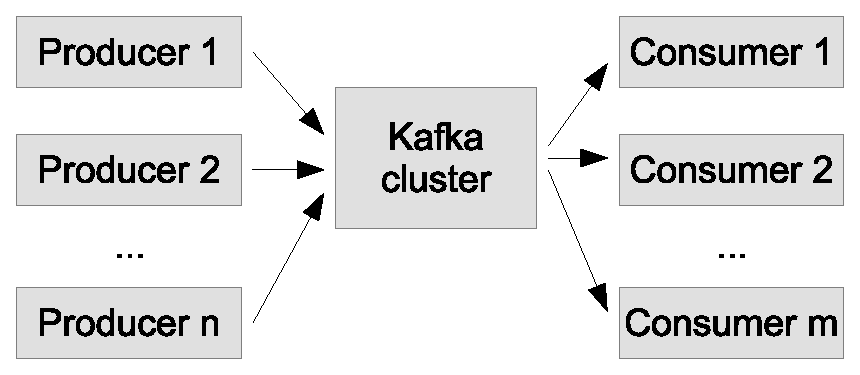
\includegraphics [width=0.5\textwidth]{images/kafka_structure}
  \caption{Kafka structure}
  \label{fig:kafka_structure}
\end{figure} 

\mnote{Kafka topic}
The core abstraction in Kafka is \textit{topic}.
One topic aggregates messages of one type.
For example, the system tracks the user activity, e.g. the number of times he opened a particular application or visited a particular website.
All these records are stored in the topic 'User activity'.
It is recommended to have a small number of topics (no more than a thousand).
However, each topic can contain  billions of messages.

One topic is a log that is spread over a cluster of brokers.
Every Kafka broker consists of zero or more partitions.
Figure~\ref{fig:kafka_topic_structure} illustrates the topic structure.
Kafka continually appends messages to the partitions.
Each partition represents an ordered sequence of messages that are uniquely identified by ids.
This id is called the \textit{offset}.
The sequence of messages is immutable and can only be extended by addition of new messages.
Besides appending, system provides one more operation: messages fetching.
Messages can be obtained from a particular partition, if a beginning message id is specified.
Kafka has an API for these operations, that can be used in different programming languages.

To provide fault tolerance, Kafka replicates each partition across several servers in a Kafka cluster.
One of these servers is a 'leader' and others are 'followers'.
The leader is responsible for handling all read and write requests.
The followers only replicate the leader.
For load balancing each server is simuntaneously a leader and a follower, i.e. for some of its partitions it acts as a leader and for others - as a follower.

The follower acts as a normal consumer, receiving data from the leader and applying it to its log.
Only when all the replicas received the message it is considered to be 'committed' and can be delivered to real consumers.
This guarantees that no message is lost even in the case of the leader failure.
A consumer always receives a message that is committed to the Kafka cluster.
A producer can wait until the message is committed or not, depending on the application logic.

To choose the leader, Kafka maintains a dynamic set of in-sync replicas (ISR).
Only these replicas can participate in the leader elections.
All these nodes must receive a message to consider it to be a committed write.
ZooKeeper stores the ISR set and tracks every change of its membership.
When a Kafka cluster has \textit{n}+1 replicas, it can sustain \textit{n} failures without any problems.

% �������� �������� ��� ��� � ������� ������ ����� ��� ���
%[reference: http://kafka.apache.org/documentation.html]
\begin{figure}[h]
  \centering
  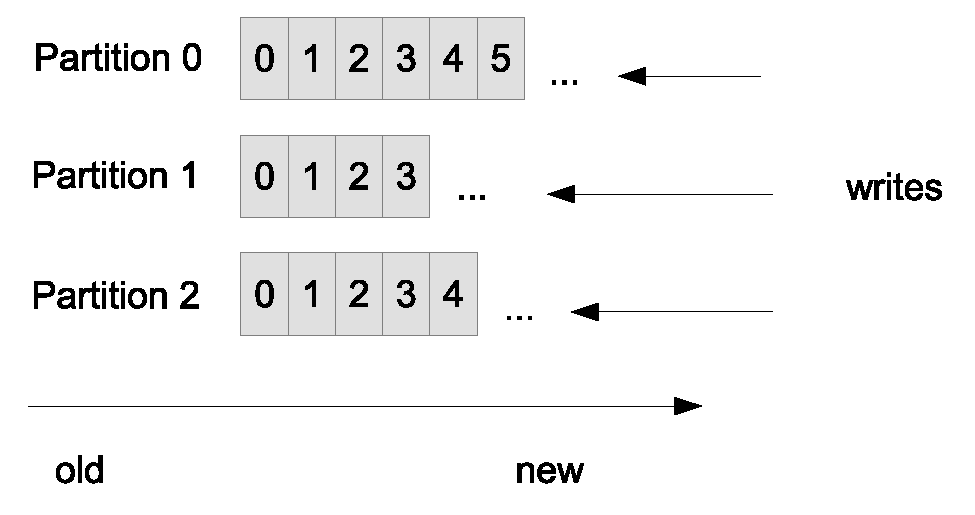
\includegraphics [width=0.5\textwidth]{images/kafka_topic_structure}
  \caption{Kafka topic structure}
  \label{fig:kafka_topic_structure}
\end{figure} 

Kafka uses a publish/subscribe mechanism to establish a communication process between producers and consumers of data.
One subscriber consists of a group of processes that run as a cluster.
Only one machine in this cluster obtains messages from Kafka.
Moreover, it consumes data from a specified partition.
Therefore, the subscriber parallelism depends on the number of partitions of the topic.
Kafka uses ZooKeeper to add or remove nodes from the broker and consumer groups.
It helps to rebalance the load automatically.

The fact that each partition has only one consumer makes it easier to store the metadata about what has been already consumed.
The consumer process just needs to store the last acknowledged message id.
Kafka uses 'at-least-once' semantic for message delivery.
It means that if the cunsumer process crashes, it reprocesses some messages from its partition one more time. 

There are two ways to balance load over Kafka brokers for message producers.
On the one hand, it can be done randomly.
On the other hand, application can supply a key that can be used to hash messages for partitioning.
The latter way guarantees the order of messages between partitions, that is not provided by Kafka.
Also it helps distributed consumers to make in-process aggregation.
In this case a consumer can obtain data from a particular partition, knowing that it contains a part of information it needs.  

For enhancing throughput Kafka introduces three techniques. 
First, it partitions data to production, consumption and brokering parts.
Second, it batches messages to chunks to send them together.
Third, it shrinks the data to decrease the amount of data that should be sent.

\mnote{batching}
The Kafka producer can send messages in synchronous or asynchronous ways.
In asynchronous mode small messages are collected into batches.
This allows to send data in chunks over the network. 
As it is done on application level, it is possible to control the batch size and the maximum time of holding the message.
Kafka allows to group messages from low-volume topics and high-volume topics together, reducing the amount of small requests.
On the filesystem level the mechanism of pagecache is used to buffer writes.
Kafka allows to delay the flush to disk again on the application level.
Similarly, it gives a control over the message boudaries and makes possible to have different policy for different topics.
Batching is also useful on the consumer side.
The client specifies the starting message id and the maximum buffer size it can receive at one time.
Kafka provides a possibility to combine data from several topics in one request.

\mnote{shrinking}
There are two techniques of data shrinking: via serialization and via compression.
Kafka associates schemas with the topics to extract the repeated structure from the messages.
Along with serialization, these schemas can be used to provide the compatibility and integration facilities.
The popular software that is used in combination with Kafka for serialization is Apache Avro.
It is described in details later in this chapter.
Kafka is able to compress several messages into a composite set of messages.
This is done during the batching process of the Kafka producer.
Thus, the messages in the compressed form are transferred to Kafka, where thay are stored and handled also in a compressed form. 

As the data transferred through Kafka is very diverse, a uniform schema is used for every topic.
This schema is kept all the way, from Kafka producer to Kafka consumer.
The schema usage is mandatory and is automatically checked.
As the schema sometimes changes, Kafka stores all its verions.
Each message contains a schema version id with which it was created.
Every schema is thoroughly tested when registered to detect incompatibilities in a timely manner.

\mnote{system monitoring}
A special Kafka topic exists to detect the percentage of data loss.
It audits the number of messages that are sent and received within a given topic over a specified period of time.
For this purpose each producer and consumer periodically notifies the audit topic about the number of processed messages.
The timestamps are extracted from the messages, instead of using the machine time of the message processing.
It is done to deal with delays in message delivering.
Kafka provides a standalone application for monitoring that processes the data from the audit topic.
It computes the ratio of data loss and duplication and is able to produce alert messages.

Kafka can by applied in a number of ways.
First, it can serve as a message broker, allowing to separate data producers from data processing.
Second, it provides facilities for real-time monitoring.
For instance, Kafka can be used to monitor the website users activity or to aggregate some application statistical data.
Third, it can serve as a log aggregation system, that can operate a log messages stream instead of dealing with log files.
This approach decreases latency and makes easier log data collection from several sources.

\mnote{log compaction}
One more Kafka application is a distributed system commit-log, that is used for restoring the failed nodes.
For this purpose Kafka has a specific feature - a \textit{log compaction}.
The main idea of log compaction is that Kafka guarantees that for all the message keys it retains the last known value.
The simpler data retention approaches are time- or size-based.
For example, Kafka removes the log data that is older than a specified period of time.
In this case some values that change rarely can be lost.
On the contrary, log compaction guarantees that at least the last value for each key persists.
This allows to fully restore the state of the broken node.

Another property of log compaction is that it shrinks the log size, removing the old records.
Using the complete log of all changes system can restore its state to any point by re-processing all the changes from the beginning of the log.
However, this approach requires a lot of memory for storing all the changes that leads to poor performance.
Log compaction removes only those records where more recent updates with the same key exist. 
Due to this fact the exterior system does not need to read the whole log and replay all the changes in order to restore its state.
Each topic has its own retention policy, i.e. one cluster can combine time or size retention with log compaction retention.

%[reference: http://kafka.apache.org/documentation.html#majordesignelements]
Figure~\ref{fig:kafka_log_structure} presents the Kafka log structure. 
The head of the log has a sequential numeration (offset) and retains all messages.
The tail of the log has a compacted structure, that contains only selected records.
It is important to mention that the messages in the log tail keep the original offset.
Kafka assignes this offset only once when a message is written for the first time and never changes it.
Moreover, even offsets for removed records are still valid log positions.
In this case Kafka returns the next highest existing value.
For instance, in our case requests with offsets 14, 15, 16 and 17 all return data starting from 17.

\begin{figure}[h]
  \centering
  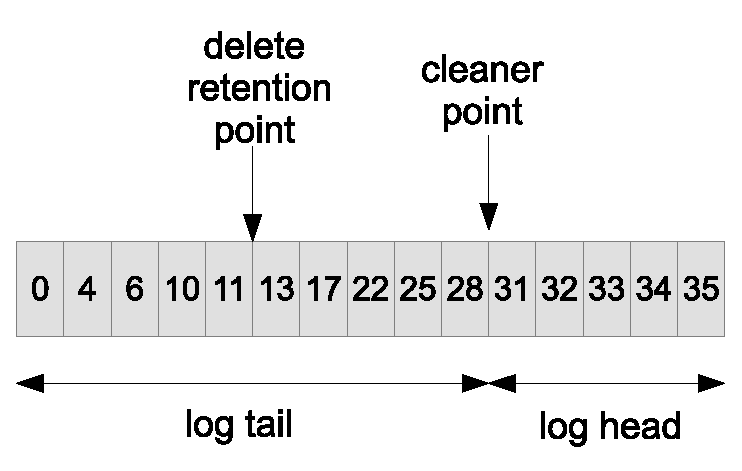
\includegraphics [width=0.5\textwidth]{images/kafka_log_structure}
  \caption{Kafka log structure}
  \label{fig:kafka_log_structure}
\end{figure} 

Compaction also performs message deletions.
If the message is marked to be deleted, all its previous versions (records with the same key) will be removed.
Deletion markers are not retained in the log after 'delete retention point' presented on the picture.

Log compaction is a background process that is run periodically.
Figure~\ref{fig:log_compaction_process} visualises a simple example.
Log compaction process posesses the following properties:
first, it guarantees the messages ordering even after compaction.
Second, the message offset is immutable and serves as a position of the record in the log.
Third, a read operation returns at least the final version for each value associated with a key.

\begin{figure}[h]
  \centering
  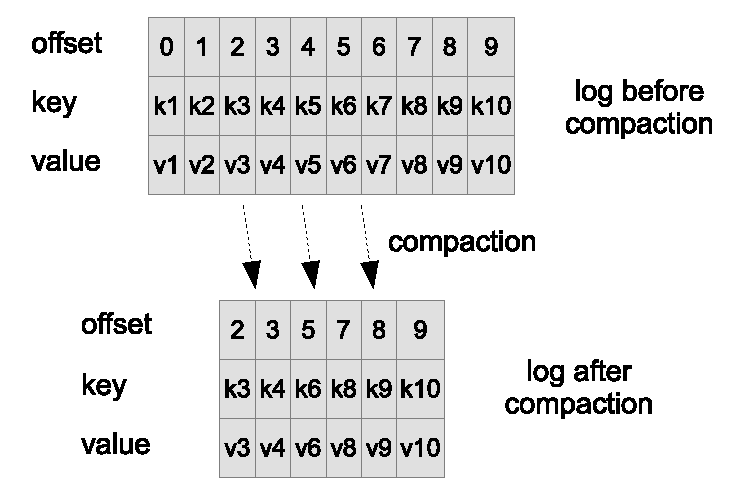
\includegraphics [width=0.6\textwidth]{images/log_compaction_process}
  \caption{Kafka log structure}
  \label{fig:log_compaction_process}
\end{figure} 

The compaction process consists of the following steps:
(1) The log is chosen, that has the biggest number of records from log head to log tail.
(2) For each key in the log head compaction process determines the last offset.
(3) The log is copied from the beginning to the end, removing the keys that occure later in the log. 
   



\subsection{RabbitMQ [VI]}

RabbitMQ is a queue messaging server \cite{RabbitMQ, AlvaroWilliams2012}.
It provides a robust, efficient and scalable message broker, that serves as an intermediate layer between sending and receiving clients.
RabbitMQ has a simple data model, that, nevertheless, offers a flexibility in the structure of data flows.
It gives an opportunity to adjust a tradeoff between throughput and reliability.
RabbitMQ fully applies Advanced Message Queuing Protocol (AMQP).

RabbitMQ is basically a delivery system, that receives messages, handles them, and then sends them to the destinations.
It is called also a \textit{broker server}\mnote{Broker server}.
It can serve messages coming from client apps to a server and backwards.
It also can be a mediator between client apps themselves.
RabbitMQ rules messages going through it, so that they are reliably stored, distributed, and then sent, possibly many times in case of absence of acknowledge from the destination.
It completely separates senders and receivers, so that they can be easily modified, removed, or added.
Figure~\ref{fig:RabbitMQGeneralStructure} shows general structure of RabbitMQ server and the flow of messages.

\begin{figure}[h]
  \centering
  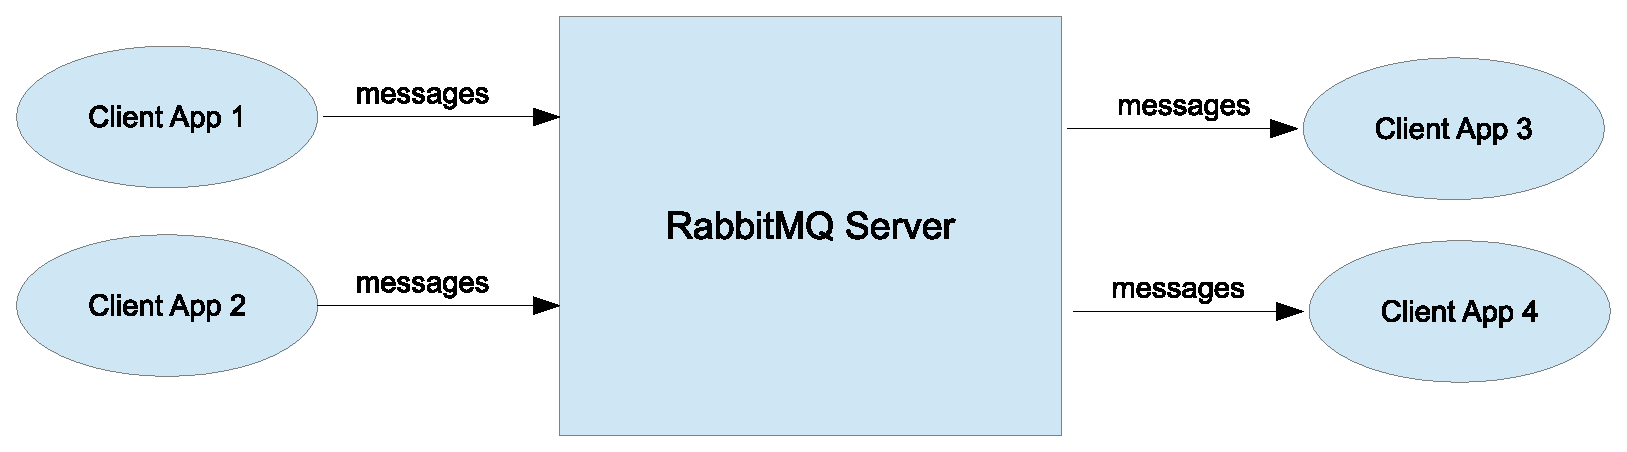
\includegraphics [width=0.9\textwidth]{images/RabbitMQGeneralStructure}
  \caption{General structure of RabbitMQ server and the flow of messages.}
  \label{fig:RabbitMQGeneralStructure}
\end{figure}

Client that sends messages is called \textit{producer}\mnote{Producer}.
Producer creates a message and sends (publishes) it to a broker.
Message consists of two parts: label and data.
Data can be anything, e.g. text, JSON object, JPG file, etc.
Label provides information about who should receive the message.
When producer sends a message, it does not wait for a confirmation from supposed receivers.
Such strategy is called fire-and-forget.
Broker acknowledges only the fact, that it has received the message properly.
It does not provide information to a sender about further life of the message. 

Client that receives messages is called \textit{consumer}\mnote{Consumer}.
Consumer subscribes to a specific \textit{queue} (we discuss queues in details below).
Broker transmits messages, coming to this queue, to all subscribed consumers.
There is no way to know who was a publisher of a message using label.
The only possibility is to sign this message inside of the data part, what is, basically, not in the scope of brokers's responsibilities.

The same application can be a producer and a consumer at the same time.
This is often a case, because application usually needs to communicate with the server or with other nodes of the network using broker server.
But it is important to mention, that there is, basically, no client and server notions in the discussed concept.
Rather it is a model of publishers and subscribers, or senders and receivers.
Broker server acts then as a middle transport layer.

For further discussion we need to describe \textit{Advanced Message Queuing Protocol} \mnote{Advanced Message Queuing Protocol (AMQP)} or \textit{AMQP} \cite{AMQP2011}.
AMQP is a protocol, that specifies common rules for messaging, queuing, publication/subscription, routing, etc.
It provides reliable, efficient, flexible, generic mechanisms for communication between clients.
AMQP is a binary protocol.
It has a set of commands, that must be implemented, e.g. \lstinline{open}, \lstinline{begin}, \lstinline{attach}, \lstinline{transfer}, \lstinline{flow}, \lstinline{disposition}, \lstinline{detach}, \lstinline{end}, \lstinline{close}.

In order to start publishing messages producer has first to connect to a broker.
It establishes TCP connection, and initializes \textit{AMQP channel} \mnote{AMQP channel} on top of it.
Such channel is only a virtual connection.
Producer can create many AMQP channels in parallel using one TCP connection.
This is useful, when for example one application needs to send many messages to the server from different threads.
It would be then very expensive to establish separate TCP connection for every thread.

Another important element of RabbitMQ broker server is Queue\mnote{Queue}.
It stores messages that are still not delivered.
Also, queue is a named object, and the name is an identifier for consumers, that want to subscribe to this queue.
There are two ways for a consumer to receive a message from the queue.
The first one is to subscribe to a queue and receive all messages that comes in it automatically.
This creates an AMQP channel, that is then used during the whole time of listening.
The second one is to retrieve a single message from a queue.
Consumer acknowledges received message to a broker.
In some cases it can reject message, for example when an error during its processing occured.
It is then important to specify (rejecting the message), that message must be sent to this consumer once more.

Consumers and producers can create queues.
Consumer must be unsubscribed from any other queue, declaring a new one.
Creating a queue, the one who does it must specify its name (or say to a broker to put random one and return it).
The name is important for producers, that want to publish to this queue.
There are two parameters to mention, that can be also specified.
The queue can be declared as exclusive, what means that only creating consumer is allowed to listen from it.
Another propery is auto-deletion, that says to a server, that queue must be deleted after the last consumer unsubscribes from it.

\textit{Exchange} \mnote{Exchange} is a component of RabbitMQ broker server that completes the whole picture.
Exchange is a place to where producer sends a message.
It is then redirected using specific rules to a particular queue.
Those rules are called \textit{routing keys}\mnote{Routing keys}.
It is said, that queue is bounded to an exchange by a routing key.
Each message that producer sends to a broker, has a routing key in its label.
Broker server tries then to match it with its bindings, to put the message in a proper queue.

There are four types of exchanges in RabbitMQ: direct, fanout, topic and header.
The difference between them is in the routing algorithm.
\textit{Direct exchange} simply matches routing key with the queues' names.
The messages goes then to the corresponding queue, always to only one among existent.
In the broker server there is always a default direct exchange, but it is possible to create more in case of specific needs of a system.
\textit{Fanout exchange} puts a message to all queues bounded to it.
It is useful, when the message must cause several different reactions.
\textit{Topic exchange} allows to send messages from different sources to the same queue, and to send messages from one source to several queues.
It is the most flexible and powerful type of exchange.
Different interesting messaging scenarious can be realized via topic exchange.
\textit{Header exchange} is similar to direct exchange, but rarely used, and we do not discuss it here.

Important concept in RabbitMQ is \textit{virtual host}\mnote{Virtual host}.
It is, basically, a virtual machine inside RabbitMQ server, that serves as a separate brocker.
This concept allows to separate different systems having the one RabbitMQ server.
Each virtual host has its completely own set of exchanges, queues and bindings.
It is easy to move virtual host from one RabbitMQ server to another, without necessity to think about what belongs to which brocker.

RabbitMQ provides \textit{durability} \mnote{Durability} of brocker's structure and exisiting messages.
If a machine with the RabbitMQ server goes down, or brocker just crashes - all exchanges, queues and messages inside will be recovered after restart.
But this mechanism is off by default, and must be switched on, in case durability is important.
To achieve this for every exchange and queue should be set to true parameter \lstinline{durable}.
Also, every message must have a \textit{delivery mode} set to 2, what informs the brocker, that it must be persisted in case of crash.
Broker writes then all needed for recovering information to a persistency log file.
It is important to remember, that durability and persistency affect efficiency, that is why they are switched off by default.
\subsection{Avro [SP]}
\label{subs:avro}

Data should be structured when it is transferred over the network.
Data objects are converted into some form, in which they can be stored or transferred and later be reconstructed in a new environment.
This process is called serialization.
The naive serialization approaches are XML or JSON.
Drawbacks of these formats that they require too much space for storing, because the data is kept it a text form.
The better solution is to use binary format for serialization and Apache Avro is one of the frameworks that use such approach.

Avro differs from the other serialization frameworks in that it does not require the code generation on receivivg.
It even allows to efficiently sort binary-encoded data without deserialization.
Also Avro supports easy schema changes, because it stores both old and new schemas and can associate fields with each other using their names.
This framework provides two types of encoding: binary encoding and using JSON.

Avro uses \textit{schemas} that are defined using JSON.
It needs a schema for serialization and in most cases this schema is transmitted along with the data.
Thus the receiving application does not need to store schemas for deserialization.
However, in some scenarios the transmission of schema is redundant, because both sides have the full schema stored locally.
In this case it is possible to transmitt only a binary representation of serialized objects.

The schema can contain both primitive and complex types.
Primitive types include: \textit{null}, \textit{boolean}, \textit{bytes}, \textit{int}, \textit{long}, \textit{string}, \textit{float} and \textit{double}.
Complex types are: \textit{record}, \textit{array}, \textit{enum}, \textit{union}, \textit{map} and \textit{fixed}.
Listing~\ref{lis:example_avro_schema} illustrates the example schema.
One schema files stores only one schema definition.

\begin{lstlisting}[caption=Avro schema (example), label=lis:example_avro_schema]
{
  "name":"AppInstall",
  "namespace": "example.avro",
  "type":"record",
  "fields":[
     { "name":"id", "type":"long" },
     { "name":"userId", "type":"long" },
     { "name":"time", "type":"long" },
     { "name":"appName", "type":"string" },
     { "name":"packageName", "type":"string" }
  ]
}
\end{lstlisting}

Avro uses an \textit{object container format} for storing objects in a file.
A file has a specified schema, that consists of blocks with synchronization markers between them.
Blocks contain data objects and can be compressed.
Synchronization markers allow to split file for processing it with MapReduce.
Moreover, Avro file comtains metadata section, where it stores a schema.

A file has the following structure: it has a header and one or several file data blocks.
The header contains information about encoding type and file metadata.
Metadata stores the schema and a type of codec that is used for compressing.
'null' codec type means that the data is uncompressed, 'deflate' codec uses the deflate algorithm.
The file data block stores information about the number of objects it contains, their sizes in bytes after compression, the serialized objects themselves and a synchronization marker.
This additional data helps to detect corrupted blocks.

Avro provides a \textit{Remote Procedure Call} (RPC) interface for implementing data exchange between a server and a client.
RPC protocol is defined using JSON.
Its attributes include a \textit{messages} object, that specifies the messages that are exchanged.  
\textit{Message} is a byte sequence, that is transmitted using a transport mechanism.
Transport system sends requests and receives responces.

Transport can have a stateless or stateful design.
\textit{Stateless} means that a server does not store any information about a client state.
The client transmitts all the needed data in every request message.
In \textit{stateful} design the server keeps the persistent client state.
This approaches has two problems.
First, the server should have a mechanism to discard client state at some point.
It is not possible to store the states of all the client for unlimited period of time.
Second, the server should be able to restore the client state in the case of the server crash.
This makes the process of server-side implementation complex comparing to sateless design.
However, stateful design results in better performance.
Figure~\ref{fig:stateful_stateless} represents the stateful and stateless schemas.

\begin{figure}
  \centering
  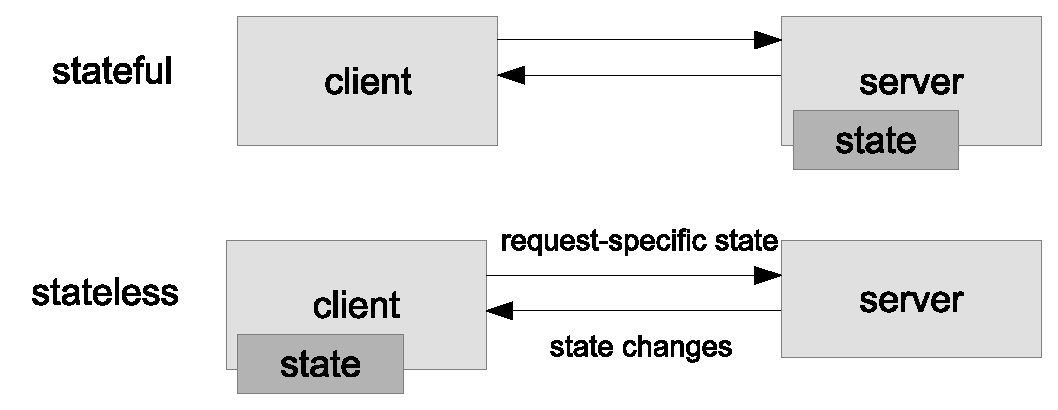
\includegraphics [width=0.7\textwidth]{images/stateful_stateless}
  \caption{Stateless and stateful design}
  \label{fig:stateful_stateless}
\end{figure}

An example of stateless transport method for Avro is HTTP.
In this case all Avro messages share the same URL at an HTTP server.
The 200 (OK) response code should be used by all response messages (normal and error).
Avro sends requests via the POST method.

There is an intermediate layer between messages and transport named \textit{framing}.
The main idea of framing is the partition of each message to a list of buffers.
A buffer contains buffer length followed by buffer data of this length.
Every message consists of one or several buffers.
Framing makes read and write operations more efficient.

Avro uses a handshake procedure before sending any RPC requests and responses.
It is used to make sure that the protocol definition is the same on both the server and the client side.
Only in this case the server and the client can correctly deserialize requests and responces.
To avoid extra network exchanges the server and the client stores recently used protocols in a cache.
Stateless and stateful transport differs in that the former requres a handshake before every request and response.
In contrast, the latter needs only one handshake and for the lifetime of the connection.

The handshake procedure is the following.
The client sends a \textit{HandshakeRequest} in a form \textit{(clientHash=clienthash, clientProtocol=null, serverHash=serverhash)}.
The \textit{clienthash} and the \textit{serverhash} are both the JSON protocol text, hashed with MD5.
The \textit{serverhash} contains data that the client received from the server during the last session.
If it is the first connection to this server the client tries to guess the server's hash.
The server sends in response a \textit{HandshakeResponse}.
If the received \textit{serverhash} is valid and the server knows the corresponding protocol to this client, the response has a form \textit{(match=BOTH, serverProtocol=null, serverHash=null)}.
In this case the connection is confirmed and the server can send a response message.
If the \textit{serverhash} is not valid, but the server knows the client protocol, it answers with \textit{(match=CLIENT, serverProtocol=serverprotocol, serverHash=serverhash)}.
It also allows the server to send the response data to the client.
However, the client must replace its nonvalid \textit{serverhash} data with that received from the server and process the response using the received protocol.
When the server is not aware of the client's protocol it received, it response with \textit{(match=NONE)}. 
Then the client re-sends its request extended by \textit{clientProtocol} value and the server response with \textit{(match=BOTH)}.

To determine the identity of the schemas stored on the client and the server side, Avro uses \textit{Parsing Canonical Form}.
It is a transformation, that removes data, irrelevant for the comparison, and normalizes the JSON text.
This canonical form can be used to create a fingerprint (an integer that serves as a unique id for a schema). 

 


\subsection{Thrift [VI]}
\label{subs:thrift}

Thrift is a framework for communication between different languages \cite{Slee2007, Thrift}.
It extracts parts of languages, that require the most usage in the interprocess interaction.
Thrift provides all basic data types, that are common for most of languages.
It separates data representation, transportation, and processing of input and output streams from each other.
Thrift has code generation tools, that produce code for all supported languages having once written definition of communication in Thrift.

Thrift has been developed at Facebook, as a result of a demand in a simple, high-performance bridge between different languages.
Solutions that were present before were too slow and clumsy, or just too limited in data types and communication needs.
Facebook had several requirements to Thrift, that it fulfilled in the implementation.
The first one is the common data type system, that saves programmer from using specific Trift data type or from writing specific serialization.
The second is transport mechanism, that separates data exchange from other layers of the program.
Next is a protocol, that defines how data is serialized to be transported.
Versioning, that allows to alter data structures or add arguments to functions without interrupting functioning of the system.
Processing of data streams, that is responsible for management of raw data, coming from the input stream, or going to the output stream. 

Thrift has a \textit{type} \mnote{Types} system, that allows programmer to code in native data types of the language, he uses.
It also saves him from writing any kind of serialization of his data structures or classes for transportation.
The Thrift IDL (Interface Definition Language) allows to describe in a file all data structures, that are to use in the interaction with another program, in a clear and compact way.
Thrift's type system contains only common types, that exist in almost any programming language.
The base types are: \lstinline{bool}, \lstinline{byte}, \lstinline{i16}, \lstinline{i32}, \lstinline{i64}, \lstinline{double}, \lstinline{string}.
All integer types are signed integers.
Facebook's developers decided, that there is no much use of unsigned integer.
They are always converted to signed integers in arithmetic operations.
Also there are languages, that do not support them at all.

Thrift supports four complex structures to define: structs, containers, exceptions and services.
\textit{Struct} corresponds basically to a class in any object-oriented language.
It allows to define indexed fields with default values.
In general, notation of structs is similar to a C struct definition.
\textit{Containers} correspond to commonly used containers in all languages, namely \lstinline{list<type>}, \lstinline{set<type>}, and \lstinline{map<type1, type2>}.
For example, in Java their mappings are \lstinline{ArrayList}, \lstinline{HashSet} and \lstinline{HashMap}, correspondingly.
The type of a container's element can be any supported type of Thrift, including structs and other containers.
\textit{Exceptions} are essentially the same as structs, but they derive base exception class in each particular language.
\textit{Sevices} correspond to interfaces or abstract classes (pure virtual class in C++) in programming languages.
Listing~\ref{listing:ThriftStructures} shows examples of notations of these Thrift's components.
Listings are taken from \cite{Slee2007} and modified.

\begin{lstlisting}[float=h, caption=Notation of Thrift's data structures., label=listing:ThriftStructures]
struct Example
{
	1:i32 number=10,
	2:i64 bigNumber,
	3:double decimals,
	4:string name="thrifty",
	5:list<i32> listOfVals,
	6:map<string, list<i32>> combinedMap
}
service StringCache
{
	void set(1:i32 key, 2:string value),
	string get(1:i32 key) throws (1:KeyNotFound knf),
	void delete(1:i32 key)
}
\end{lstlisting}

\textit{Transport} \mnote{Transport} layer in Thrift is responsible for managing data transportation issues.
It does not specify exact transport protocol or method, rather it provides common interface.
For example it can define a communication using network socket, or writing to a file or database.
Basically transport requires only to know how to read write data, and does not need to know the source and the destination.
The main methods of the transport interface are: \lstinline{open}, \lstinline{close}, \lstinline{isOpen}, \lstinline{read}, \lstinline{write}, \lstinline{flush}.
There are several implementations of Thrift's transport interface, namely \lstinline{TSocket} for TCP/IP communication, \lstinline{TFileTransport} for writing to the file, \lstinline{TMemoryBuffer} that allows to read and write directly to memory allocated for the process.

\textit{Protocol} \mnote{Protocol} layer in Thrift separates data representation and transportation.
It provides specific structure of messaging, but it need not to be aware about how data is encoded, as XML, ASCII or binary format.
Data only must to support a set of operations defined by a protocol's interface.

Interface of Thrift's protocol contains two types of methods: for messaging and for encoding particular types of data and structures.
It has many methods, several examples are: \lstinline{writeMessageBegin(name, type, seq)}, \lstinline{writeMessageEnd()}, \lstinline{writeStructBegin(name)}, \lstinline{writeStructEnd()}, \lstinline{writeFieldBegin(name, type, id)}, \lstinline{writeFieldEnd()}, \lstinline{writeBool(bool)}, \lstinline{writeI32(i32)}, \lstinline{writeDouble(double)}, \lstinline{writeString(string)}.
There are similar reading methods, that we omit here for conciseness.
Basically, every writing function has it reading pair.
Thrift supports streaming writing of data, that allows to write and read data simultaneously.
For this sake each field of a structure contains its type identifier, what allows to write/send the value as an atomic element to the stream.
Facebook has implemented for its needs an efficient binary format, that is in use in many of its backend services.

Thrift has a \textit{versioning} \mnote{Versioning} model, that allows to change and improve data structures and interfaces, and read old data without special additional adjustments.
To provide this feature, Thrift uses identifiers for fields and methods' arguments.
Each field in the structure has then a field that is unique.
On deserialization, generated code recognizes old fields and simply omits them.
For the case, when there is no expected field, Thrift provides each structure with a so called \lstinline{isset} object.
It specifies for each field whether it is present in the structure.
Reading the structure, it is always explicitly to check \lstinline{isset} for a particular field to read.
Protocol and transport interfaces of Thrift also support versioning, so that developer can change them to fit better his needs.
Listing~\ref{listing:ThriftIsset} shows an example of \lstinline{isset} structure.

\begin{lstlisting}[float=h, caption=Example of isset structure., label=listing:ThriftIsset]
class Example
{
	public:
		Example() :	number(10),	bigNumber(0), decimals(0) {}
		int32_t number;
		int64_t bigNumber;
		double decimals;
		struct __isset
		{
			__isset() :	number(false), bigNumber(false), decimals(false) {}
			bool number;
			bool bigNumber;
			bool decimals;
		} __isset;
...
}
\end{lstlisting}

%Case Analysis
%Protocol/Transport Versioning

Thrift provides \textit{RPC} \mnote{RPC} using interface \lstinline{TProcessor}.
The ides is to divide complex systems into many simple communicating elements, that works with inputs and outputs.
In most case it is only one input and one output that are to handle.
On the Listing~\ref{listing:ThriftTProcessor} is an interface of the \lstinline{TProcessor}.

\begin{lstlisting}[float=h, caption=Thrift's TProcessor interface., label=listing:ThriftTProcessor]
interface TProcessor
{
	bool process(TProtocol in, TProtocol out)
		throws TException
}
\end{lstlisting}

%Generated Code
%TServer The Thrift core library has already implemented the \lstinline{TServer} abstraction.

Thrift's \textit{implementation} \mnote{Implementation details} supports many commonly used programming languages, e.g. Java, C++, Python, PHP, Ruby, etc.
Facebook deploys servers mostly using C++, Java and Python.
Apache web server uses Thrift to provide transparent communication between backend and frontend using \lstinline{THttpClient}.
Names of RPC methods in Thrift are sent as strings, what is though more bandwidth consuming, but ease implementation and matching of versions of interface definitions.

% more details about implementation

Facebook implemented many services using Thrift \mnote{Facebook Thrift Services}.
Facebook Search service uses Thrift for realization of the underlying protocol and transport layer.
Also Facebook Search service comprises components written on different languages.
Web-part implemented using PHP, search engine using fast C++, statistical and testing components using Python.
All these components need to communicate in a fast, robust and simple way, and Thrift fulfils these properties.

\section{Real-time Data Processing Systems}

Efficient processing of big volumes of data is a crucial point for any big data system.
It must be easy to model, develop and maintain.
This section describes two data processing frameworks - \textit{Storm} and \textit{Spark}.
They have different computational models, but allow execution of the same computations.
The difference between them is that Storm is a truly real-time processing system, whereas Spark works essentially with batches, and has a streaming extension on top of batch computations.

\subsection{Storm [SP]}

Batch processing is not applicable for real time computing.
Hadoop, the best known tool for batch processing, is helpless when it is needed to handle streaming data and obtain immediate result.
The main advantage of real time processing, the guaranteed time delay between a request and a result can be broken simply because the waiting time for the next batch is too long.
Therefore new systems, designed for real-time processing, have appeared.
One of such systems is an open source project named \textit{Storm}.

Storm is a \textit{complex event-processing} (CEP) system.
Complex event processing means gathering data from different sources, combining it and making conclusions from it.
For example, such system keeps track of significant changes in traffic reports or stock market feeds and immediately responds to them. 

Storm is implemented in a dialect of the Lisp language named Clojure.
Clojure is a functional language like Lisp, but it also supports multithreaded programming.
Clojure runs on the Java Virtual Machine, however applications within Storm can be written in Java, Scala, JRuby, Perl and PHP.
Moreover, one can use a Structured Query Language adapter for streaming data directly into Storm topoloy.

\mnote{Storm architecture}
The Storm cluster has a master node called \textit{Nimbus} and \textit{worker} nodes.
Nimbus assignes tasks for workers and monitors failures.
There is a deamon called \textit{Supervisor} on every worker node.
The supervisor is responsible for starting and stopping worker processes assigned by Nimbus.
ZooKeeper coordinates the interaction between Nimbus and Supervisors.
It stores the state of all the nodes, making the system stable to failures.
If any of the nodes is killed, ZooKeeper immediately restarts it, enhancing Storm cluster stability.
ZooKeeper is described in more details later in this chapter.

The basic concept of Storm is a \textit{topology}.
It is a graph of computation, that shows how data should be processed and passed between the nodes.
One can implement a topology in any programming language, because topology definition is a Thrift structure.
Thrift is a framework that allows to develop cross-language services.	

The data stream consists of an unbounded set of \textit{tuples}.
A tuple can contain both standard data types (integer, float, byte array) as well as user-defined types.
Every stream has its own ID.
The sources of streams called \textit{spouts}. 

The next important Storm primitive is \textit{bolt}.
Figure~\ref{fig:storm_architecture} shows the interaction between spouts and bolts.
The stream of tuples originates from a spout and goes through a sequence of bolts.
Every bolt performs a transformation on incoming data stream, like aggregating, filtering, or interaction with external parts such as databases.
A bolt can receive information from several spouts and stream it to multiple bolts.

\begin{figure}
  \centering
  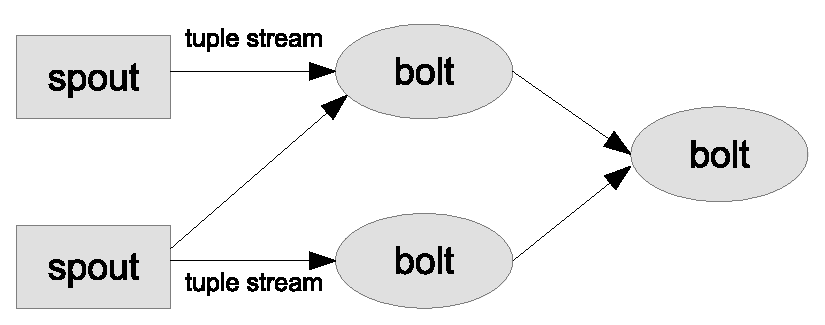
\includegraphics [width=0.5\textwidth]{images/storm_architecture}
  \caption{Storm architecture}
  \label{fig:storm_architecture}
\end{figure}

For example, MapReduce word counting example can be easily implemented with Storm.
Such system counts how many times each word occures in a given input data.
In the case of Storm one needs 
(1) a spout to generate text data, 
(2) one bolt to implement the Map function for word tokenisation and 
(3) one bolt to implement the Reduce function for aggregation the amounts of words occurences. 

Storm allows to group the stream of tuples in different ways.
For instance, shuffle grouping randomly distributes tuples to bolts such as each bolt receives approximately the same number of tuples.
Field grouping partitions tuples according to contained fields.
Also other grouping methods exist, including the custom grouping.

The Listing~\ref{lis:simple_storm_topology} represents a simple topology.

\begin{lstlisting}[caption=Simple Storm topology, label=lis:simple_storm_topology]
java TopologyBuilder builder = new TopologyBuilder();
builder.setSpout("myspout", new TestSpout(), 10);
builder.setBolt("mybolt1", new TestBolt(), 3) .shuffleGrouping("myspout");
builder.setBolt("mybolt2", new TestBolt(), 2) .shuffleGrouping("mybolt1");
\end{lstlisting}

Here topology consists of one spout and two bolts.
The stream of tuples originates from \textit{myspout}, then it is passed to \textit{mybolt1} and finally to \textit{mybolt2}.
In both cases tuples are grupped using the schuffle grouping method.
The integer numbers in \textit{setSpout} and \textit{setBolt} define the amount of parallelism for the node.

The implementation charasteristics of Storm lead to high performance and guaranteed fault tolerance.
It uses ZeroMQ for passing messages between the tasks.
Messages are automatically serialized and deserialized to Storm primitive types.
The usage of this message queue helps to avoid intermediate queueing, thus improving performance.
Furthermore, Storm guarantees the processing of every tuple.
In the case of a fault during message processing, a tuple is replayed from the spout.
There is also a fault detection mechanism on task level, when the failed task is quickly reassigned to restart the processing.
Storm has supervisors to manage the processes, that leads to efficient usage of resources.

Storm cooperates with message queue systems in such a way that every message is fully processed.
It builds a tuple tree, that reflects the motion af all the tuples.
Only when every message in the tuple tree is processed, a tuple is considered to be fully processed.

To give an example, let us take a message queue that supplies a spout with messages.
When the spout takes a message from the queue, the message state changes to 'pending'.
In this state it cannot be sent to other consumers.
Moreover, all the messages in pending state are returned to message queue if their consumer disconnects.
Storm assignes a unique id to the message, if it is not given by the message queue.
Using this id Storm can keep track of this message during processing.
The system receives this message when the \textit{nextTuple} method of the spout is called.
The spout emits the message along with its id to the consuming bolts.
When a tuple is fully processed, the \textit{ack} method of the original spout is called. 
In the case of time-out Storm calls the \textit{fail} method of the same spout.
Only when \textit{ack} or \textit{fail} method is called, the spout sends an ack or fail message to the message queue.
The message queue cancels the pending state of the message, taking it off the queue in the case of success and putting it back otherwise.

Storm can process not only the tuple trees, but also directed acyclic graphs.
It happens when an output tuple is anchored to several input tuples.
\textit{To anchor} means to specify a link in the tuple tree.
Multi-anchored tuples often appear during streaming aggregation or joining.
 
As it was mentioned, Storm tracks every tuple using its unique id.
Additionally, as each tuple exists within a tree, it knows all the tuples ids of this tree.
For example, if a bolt emits a new tuple, this tuple carries the ids of spout tuples received by this bolt along with its own id.
Such storage mechanism is used	because when the tuple is acked or failed, it should inform Storm about its dependencies to restore the state of the tuple tree.  

The acker task is responsible for acking the tuple.
First, Strom stores the mapping between an acker task and a spout tuple id.
As every tuple keeps ids of spout tuples in the tree it exists within, it knows the acker tasks it should communicate with.
A tuple informs an acker task when the tree is fully processed and the tuple is acked.
Second, the acker task should send a complition message to the spout task that emitted this tuple.
For this purpose, on creation of a new tuple a spout task notifies the appropriate acker task that its task id is linked to that spout tuple.

For acker task tracking the huge tuple trees explicitly is not efficient.
Thus Storm uses a special tracking strategy.
An acker task stores a map: on the one side it has a spout tuple id and on the other side a pair of values.
One of the values is a task id the spout tuple originates from, and the other is an 'ack val', the 64 bit number.
The 'ack val' represents the state of the tuple tree without storing it in memory.
This number is a result of XOR operation on all created and acked tuple ids of the tree.
Therefore, when the 'ack val' is equal to zero, it means that the tree is completed.
\subsection{Spark [VI]}

Spark is a framework for distributed processing of data \cite{Zaharia2010} \cite{Zaharia2013} \cite{Spark1} \cite{Spark2}.
It works with large datasets and streams of data, and lets to make complex queries on this data.
It consists of two parts: Spark engine that allows to process data in a batch fashion, and Spark streaming that extends Spark engine to handle fast coming streaming data.
Spark is simple, efficient and fault-tolerant.
It abstracts programmer from details of how processing distributes across cluster, and how robustness is achieved.
It shows results that surpass Hadoop in efficiency in 10 times.

Spark has several abstractions to represent data and streams.
Using them it is easy to write simple, short and robust code, that implements complex algorithms on batch and streaming data.
The first one - Resilient Distributed Dataset (RDD) - an object, distributed in the cluster, that contains data to process.
Another one is a Shared Variable - variable, that can be used among the cluster as a counter or a lookup table.
The last abstraction is a Discretized Stream (DStream) - representation of a data stream in a distributed fashion based on RDD objects.

%\subsubsection{Data model and batch processing}

\textit{Resilient Distributed Dataset} \mnote{Resilient Distributed Dataset} (RDD) is the main notion in Spark, that represents dataset in a distributed fashion.
RDD is essentially a readonly collection of elements.
It is fault-tolerant, so that if one partiotion is lost, the whole collection can be recovered.
RDD does not need to exist physically on the cluster nodes.
Instead, it is a lazy object, that can lay in a robust data storage, and be computed on the fly, when computations require particular pieces of data.
Figure~\ref{fig:RDDArchitecture} shows general architecture of an RDD object.

\begin{figure}[h]
  \centering
  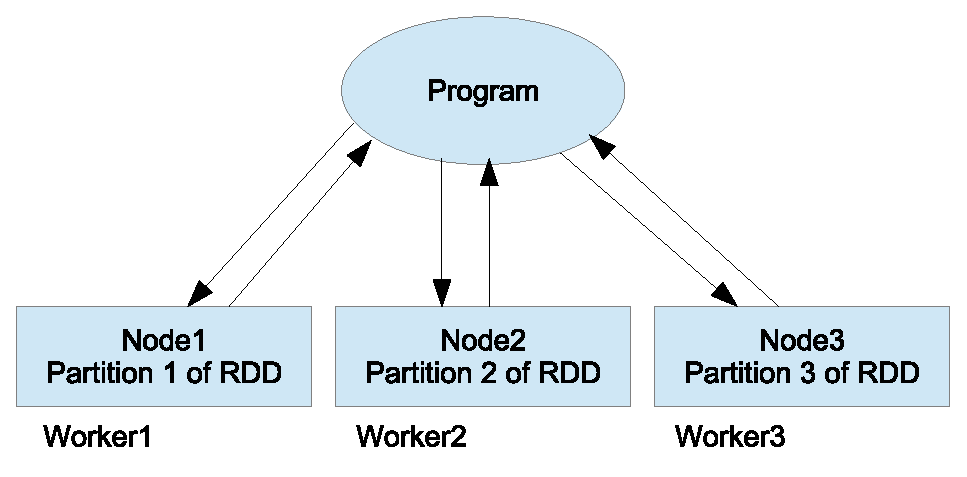
\includegraphics [width=0.7\textwidth]{images/RDDArchitecture}
  \caption{General architecture of an RDD object.}
  \label{fig:RDDArchitecture}
\end{figure}

There are two methods how to obtain an RDD object: parallelizing exisiting collection in the driver program, and using external dataset.
Existing collection is any collection of data, e.g. array, list, set, etc., that is directly handled in the program.
Creating an RDD object in this way, elements of a collection are copied to a distributed dataset, that can be used then in parallel.
It is possible to specify the number of slices, that is the number of tasks, each machine in the cluster will then execute for this collection.
External dataset is an external file.
It can reside in the local file system, and in the distributed file system like HDFS.
The simple example of processing data from the external text file in Spark, is to count the sum of lines' lengths using functions \lstinline{map} and \lstinline{reduce} of an RDD object. 
Additionally, it is possible to obtain RDD by transforming another RDD, or by changing persistance of an existing RDD, but this methods are derived in some sense.

RDD supports two types of operations: transformations and actions.
\textit{Trnsformation} \mnote{transformation} creates a new RDD object from existing one.
Examples of transformation are \lstinline{map}, \lstinline{flatMap}, \lstinline{filter}, \lstinline{groupByKey}, \lstinline{reduceByKey}.
For instance, a method \lstinline{map} processes each element of an RDD object using specified function, and returns a new RDD object as a result.
\textit{Action} \mnote{action} executes computations on an RDD object, and returns a value.
Examples of actions are \lstinline{reduce}, \lstinline{collect}, \lstinline{count}, \lstinline{countByKey}.
Method \lstinline{reduce} is a basic example of an action.
It aggregates all elements giving in the RDD object and return the resulting value.

Transformation in Spark is a lazy operation, in the sense that it is computed only when action operation requires its result to produce output.
This makes execution more efficient when there is a chain of transformations before final action, because the application does not receive then intermediate RDD objects, but only final resulting value, that is usually much smaller.
Nevertheless, there are cases, when it is to compute different actions on the same transformation.
Then it is meaningful to have RDD object of this transformation computed once, and to have a handle to it in the program.
For this case there is a method \lstinline{persist}, that allows to materialize RDD object.
This is also possible to persist RDD object on disk.

Fault-tolerance of Spark is based on HDFS and on the nature of RDD's realization.
As long as all data locates on HDFS, if any machine fails, all lost data can be recovered.
In case of node failure, RDD recovers itself, so that no data is lost, and processing is going without additional handling of administrator.

To initialize Spark it is first to create a \lstinline{SparkContext} object, that is responsible for a connection of the program to Spark.
It allows to specify properties of the application, and also options of how Spark should run, for example in local mode or on the cluster.
\lstinline{SparkContext} gives an access to different parameters and properties of execution environment.

\begin{lstlisting}[float=h, caption=Example of RDD usage., label=listing:RDDExampleCode, language=Java]
SparkConf conf =
		new SparkConf().setAppName(appName).setMaster(master);
JavaSparkContext sc = new JavaSparkContext(conf);
JavaRDD<String> lines = sc.textFile("data.txt");
JavaRDD<Integer> lineLengths = lines.map(s -> s.length());
int totalLength = lineLengths.reduce((a, b) -> a + b);
\end{lstlisting}

On the Listing~\ref{listing:RDDExampleCode} we present a simple program, that counts the sum length of all lines in the text file.
Example is taken from \cite{Spark1}.
Here we create an RDD object from external file, set \lstinline{map} function to count length of the each line, and set \lstinline{reduce} function to sum up lengths of lines.
Execution starts only when \lstinline{reduce} function is called, because, as we discussed, transformations are lazy in Spark.

Normally, passing arguments to a function, that executes on the nodes of the cluster, they are simply copied and there is no feedback to the driver program.
Sometimes it is useful to have global variable or lookup table, that all nodes can access.
Spark supports the notion of a \textit{shared variable}\mnote{shared variable}.
There are two types of shared variables: broadcast variables and accumulators.
\textit{Broadcast variable} \mnote{broadcast variable} represents readonly value or dataset, that is useful for all nodes as a lookup table or global predefined value.
It is copied to every node using method \lstinline{broadcast} of \lstinline{SparkContext}.
There are efficient algorithms in Spark to make this transfer fast.
\textit{Accumulator} \mnote{accumulator} is a distributed counter, that allows all nodes to add up to the global numeric variable.
It can be created using method \lstinline{accumulator} of \lstinline{SparkContext}.
No node can read this value or do anything else than incrementation, what makes its implementation easy and fast.
Only driver program is able to read accumulator's value.

%\subsubsection{Streaming processing}

\textit{Streaming in Spark} \mnote{Spark streaming} is an extension of a Spark engine, described in the previous section.
It can process data stream in a distributed manner.
Spark streaming receives data from the input stream, divides it into blocks, each represented as an RDD, and passes this sequence of blocks to the Spark engine.
It can work with different sources, e.g. message queue server (Kafka), web service (Twitter API), or regular TCP socket.
Processed data can be there stored to the filesystem or database.
The main abstraction for streaming processing in Spark is a Discretized Stream or DStream.
It is internally a sequence of RDDs.
Several DStreams can be combined into one chain for application more complex algorithms. 

\textit{Discretized Stream} or \textit{DStream} \mnote{Discretized Stream (DStream)} is the main abstraction in Spark streaming.
DStream can be the input stream, as well as intermediate stream, generated after processing of input stream of data.
It is essentially a chain of RDD objects, and provides a stream of data, that is to process by Spark.
Each RDD represents batch of data in the period of time, that is specified in the \lstinline{SparkStreamingContext}.
Figure~\ref{fig:SimpleDStream} depicts simple DStream.

\begin{figure}[h]
  \centering
  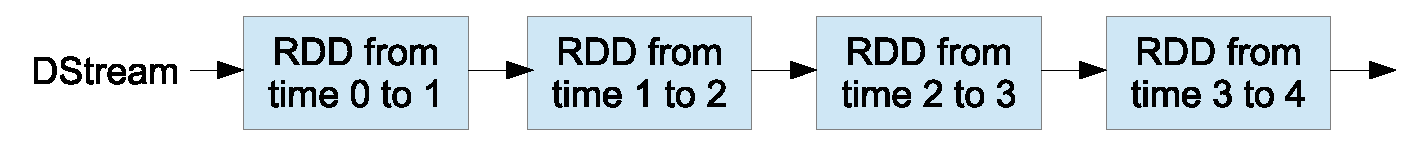
\includegraphics [width=1.0\textwidth]{images/SimpleDStream}
  \caption{Representation of a simple DStream.}
  \label{fig:SimpleDStream}
\end{figure}

Every operation, applied to DStream, is applied to every RDD object in the stream.
This implies, that transformation on the DStream produces new DStream.
All these transformations are executed by Spark engine in a standard batch fashion.
Figure~\ref{fig:DStreamWithTransformation} depicts how it works.

\begin{figure}[h]
  \centering
  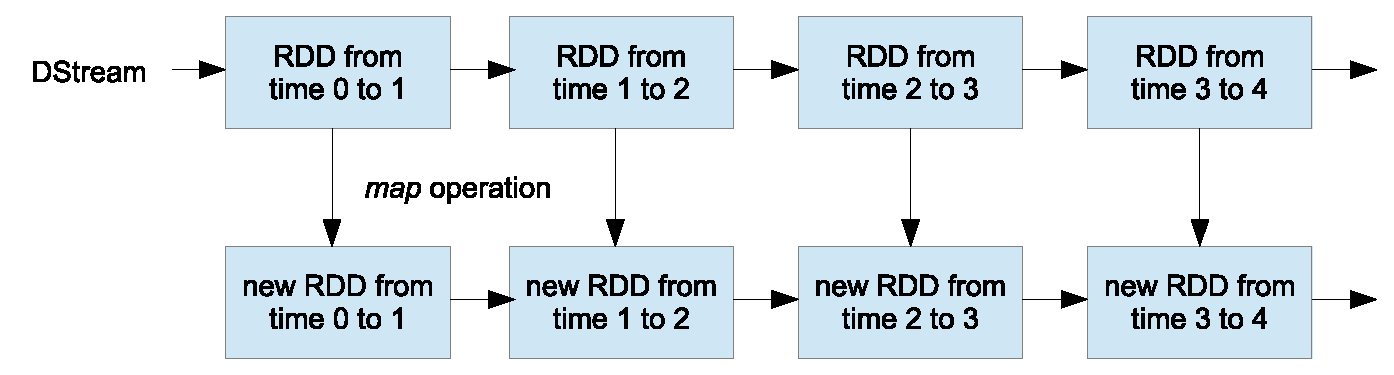
\includegraphics [width=1.0\textwidth]{images/DStreamWithTransformation}
  \caption{Transformation of a DStream to a new DStream.}
  \label{fig:DStreamWithTransformation}
\end{figure}

\textit{Input DStream} is a stream of raw data coming to Spark from the outer source.
Sources can be of two types: basic sources and advanced sources.
Basic sources are sources, that available using standard streaming context API, e.g. files or sockets.
Advanced sources are available using specific libraries, for example Kafka message queue server.
There is a notion of \lstinline{Receiver}, that is an object that receives data from the stream, put into Spark's memory, so that it is available for input DStream, associated with this Receiver.
Every DStream is responsible only for one input data stream.
Many DStreams can be created for different input streams to receive data from different data sources in parallel.
Receiver is executing as a long running task, hence it occupies one core of the processor.
This implies, that there should be more cores then receivers in the system.

There is a list of transformation to apply on a DStream.
They all are almost the same as transformations available for RDD, because DStream works on top of RDD.
The most common are \lstinline{map}, \lstinline{flatMap}, \lstinline{filter}, \lstinline{reduce}, \lstinline{reduceByKey}.

Similarly to Spark engine, it is to create \lstinline{SparkStreamingContext} object to work with Spark streaming.
It allows to adjust environment for processing, set properties like local or cluster mode, number of threads used, and many others.
One important property is the batch interval.
It defines the time of gathering data from the input stream, before creating RDD object and sending it to the Spark engine.

% must check this example
\begin{lstlisting}[float=h, caption=Example of DStream usage., label=listing:DStreamExampleCode, language=Java]
SparkConf conf = new SparkConf()
		.setMaster("local[2]").setAppName("NetworkWordCount");
JavaStreamingContext jssc =
		new JavaStreamingContext(conf, new Duration(1000));
JavaReceiverInputDStream<String> lines =
		jssc.socketTextStream("localhost", 9999);
JavaDStream<String> words =
		lines.flatMap(line -> Arrays.asList(line.split(" ")));
JavaPairDStream<String, Integer> pairs =
		words.map(w -> new Tuple2<String, Integer>(w, 1));
JavaPairDStream<String, Integer> wordCounts =
		pairs.reduceByKey((x, y) -> x + y);
wordCounts.print();
jssc.start();
jssc.awaitTermination();
\end{lstlisting}

Listing~\ref{listing:DStreamExampleCode} shows a simple example of a Spark streaming program.
Example is taken from \cite{Spark2}.
This code counts frequencies of words coming in a text data from the TCP socket.
First we create \lstinline{SparkStreamingContext} object, and specify it to work in a local mode using two execution threads.
We set a duration of gathering data from the input stream to 1 second.
In the line 3 we create DStream responsible for an input stream associated with TCP socket.
Then we apply two transformations and one action.
Transformations are \lstinline{map}-functions, so that the first one splits lines to words, and the second transforms words to pairs of the form \lstinline{(word, 1)}.
Action is a \lstinline{reduce} operation that sums up occurances of the same word.
Execution starts only when we call \lstinline{start} method of \lstinline{SparkStreamingContext}.
In the 7th line we print out partial results of the processing.
Instead, we can push results to a database or to a file, what is usually a case.

Spark streaming has a number of output operations on DStreams, that used to push transformed data to outer systems.
This can be files or databases.
Output operations actually start execution, as \lstinline{actions} of Spark engine do.
Examples of output operations are \lstinline{print}, \lstinline{saveAsObjectFiles}, \lstinline{saveAsTextFiles}, \lstinline{saveAsHadoopFiles}, \lstinline{foreachRDD}.

DStream allows to persist it in the memory, when multiple computations of the same DStream are required.
Method \lstinline{persist} of DStream object does that.
Its execution specifies that every RDD of the DStream will be persisted in the memory, as it is done for RDD in Spark engine.
For data, arriving from network, the persistence level is so, that all data is replicated to two nodes to provide fault-tolerance.

There is a mechanism of checkpointing in Spark streaming.
It allows to make snapshots of intermediate data to HDFS.
It makes computation throughput less, if set not properly.
So it must be carefully tuned.

\section{Storage Systems}

There are nowadays many different storage systems for big data management.
They have different data models and, hence, different applications.
Often they store data in a key-value manner.
In this section we consider three systems that are relevant for our work.
HDFS is a distributed file system that keeps data essentially in a tree structure in files.
Redis is a very simple in-memory key-value store.
Cassandra is more sophisticated column-style fully distributed data storage.

\subsection{HDFS [VI]}


\subsection{Redis [VI]}
\label{subs:redis}

Redis is an in-memory storage, that keeps data in a key-value fashion \cite{Seguin2012, Redis}.
It maintains data handled by a single application or by a cluster.
Redis is easy to deploy, learn and use.
It provides 5 data types, e.g. string, list, set, ordered set and hash, that are useful for different tasks, and give a powerful tool in combination.
Redis is an open source database system.

%\subsubsection{Basics}

Redis allows to create many different databases and switch between them.
Within one database Redis maintains a global map of keys to values.
The key is always a string.
It identifies piece of data, and does not represent data itself.

Redis provides many useful and simple commands to work with data.
The two simplest commands are \lstinline{SET} and \lstinline{GET}, that let to store a key-value pair into database, and to get value by key, respectively.
Listing~\ref{listing:RedisSetGet} shows an example of how to use these commands.
In this example the key is \lstinline{server:name} and the value is \lstinline{"SERVER1"}.

\begin{lstlisting}[float=h, caption=Example of usage of commands SET and GET., label=listing:RedisSetGet]
> SET server:name "SERVER1"
OK
> GET server:name
"SERVER1"
\end{lstlisting}

Redis allows to query values only by keys.
This is opposite to relational databases, where it is possible to search everything stored.
There is one exception, a command \lstinline{KEYS}, that returns all keys, stored in the database.
But it is strongly advised not to use it in production release, because it does a linear scan through all the keys, what can be very slow.
This command is rather for administrative issues.
Another point is that operation of receiving a value by a key works in a constant time, basically instantly.
This makes Redis in fact fast and useful, because grow of the database does not affect its performance.

Although Redis is an in-memory database system, it swaps data continuously to disk to provide persistance in case of application's failure.
Redis stores the database to disk every minute if at least 1000 keys have been changed.
It makes less swaps, if less keys have been changed.
It does swap completely as a snapshot.
There is though an alternative way to set Redis to make appending swaps.

%!!!!!!!!!!!!!!!!!!!!!!!!!!!!!
%Replications (can be written)
%!!!!!!!!!!!!!!!!!!!!!!!!!!!!!

%\subsubsection{Data types}

The basic data type in Redis is \textit{String}.
Keys are always strings.
Values can be of any type, but String is the most popular, because it represents atomic piece of data.
As a String it is possible to store not just something simple like name of a user or text data, but also complex objects like JSON object.
On the Listing~\ref{listing:RedisSETComplexValue} is an example of such action.

\begin{lstlisting}[float=h, caption=Usage of SET command with complex value., label=listing:RedisSETComplexValue]
> SET users:user001 '{"firstname":"john", "lastname":"smith"}'
OK
> GET users:user001
"{\"firstname\":\"john\", \"lastname\":\"smith\"}"
\end{lstlisting}

Redis provides standard commands to work with strings, e.g. \lstinline{STRLEN}, \lstinline{GETRANGE}, \lstinline{APPEND}, etc.
Storing a numeric value as a string, it is possible to work with it as with integer.
Redis has several useful commands for this case, e.g. \lstinline{INCR}, \lstinline{INCRBY}, \lstinline{DECR}, \lstinline{DECRBY}, \lstinline{SETBIT}, \lstinline{GETBIT}.
On the Listing~\ref{listing:RedisIntegerValue} is an example of working with value as with integer.

\begin{lstlisting}[float=h, caption=Working with value as with integer., label=listing:RedisIntegerValue]
> SET x 1
OK
> INCR x
(integer) 2
> INCRBY x 5
(integer) 7
> DECR x
(integer) 6
> DECRBY x 3
(integer) 3
> GET x
"3"
\end{lstlisting}

The first complex data type in Redis is \textit{List}.
List is simply an array of values identified by a key.
There are specific commands to work with lists, e.g. \lstinline{LPUSH}, \lstinline{RPUSH}, \lstinline{LRANGE}, \lstinline{LLEN}, \lstinline{LPOP}, \lstinline{RPOP}, etc.
Values of the list can be anything, not only strings.
This gives powerful tool to store complex combined data.
Listing~\ref{listing:RedisListCommands} shows basic usage of Lists.

\begin{lstlisting}[float=h, caption=Usage of List data type commands., label=listing:RedisListCommands]
> LPUSH users john mike jack
(integer) 3
> LRANGE users 0 -1
1) "jack"
2) "mike"
3) "john"
\end{lstlisting}

The next data type is \textit{Set}.
Set is an unordered array of distinct values.
There are many useful operations to work with sets in Redis, e.g. \lstinline{SADD}, \lstinline{SISMEMBER}, \lstinline{SINTER}, \lstinline{SINTERSTORE}, etc.
Set is implemented internally as a hash-table, hence, it provides constant lookup.
Listing~\ref{listing:RedisSetCommands} shows basic usage of Sets.

\begin{lstlisting}[float=h, caption=Usage of Set data type commands., label=listing:RedisSetCommands]
> SADD friends:john mike paul jack tania
(integer) 4
> SISMEMBER friends:john paul
(integer) 1 
\end{lstlisting}

\textit{Sorted set} is an extension of a regular Set, that provides order for its elements.
To order values, it uses scores.
Each value has then a score, that must be set together with inserted value.
It is possible then to lookup all values in the specific range of the score, or obtain all values in the sorted order.
Main commands for working with Sorted sets are \lstinline{ZADD}, \lstinline{ZCOUNT}, \lstinline{ZRANK}, \lstinline{ZREVRANK}, etc.
In case when it is needed to get array sorted by integers, Sorted set is a perfect data structure to do that.
Listing~\ref{listing:RedisSortedSetCommands} shows basic usage of Sorted sets.

\begin{lstlisting}[float=h, caption=Usage of Sorted set data type commands., label=listing:RedisSortedSetCommands]
> ZADD friends:john 70 mike 95 paul 92 jack 75 tania 1 dave
(integer) 5
> ZCOUNT friends:john 90 100
(integer) 2
\end{lstlisting}

\textit{Hash} is the last data type given in Redis.
Hash is essentially a hash-table, that maps strings to any objects.
It works also in constant time.
There are different commands to work with Hashes, e.g. \lstinline{HSET}, \lstinline{GHET}, \lstinline{HMSET}, \lstinline{HMGET}, \lstinline{HGETALL}, \lstinline{HKEYS}, \lstinline{HDEL}, etc.
Hashes give simple useful tool to store objects in an object-oriented way.
For example, instead of storing information about user as a JSON object, or as another string representation, it can be done using Hash.
Every field of a user is then put as a separate key-value pair.
Listing~\ref{listing:RedisHashCommands} shows basic usage of Hashes.

\begin{lstlisting}[float=h, caption=Usage of Hash data type commands., label=listing:RedisHashCommands]
> HSET users:john id 375
(integer) 1
> HSET users:john name "john"
(integer) 1
> HSET users:john lastname "smith"
(integer) 1
> HGETALL users:john
1) "id"
2) "375"
3) "name"
4) "john"
5) "lastname"
6) "smith"
\end{lstlisting}

%\subsubsection{Features}

Redis allows to use transactions to make several operations atomic.
Basically, any single operation that Redis does, is atomic, because Redis is single-threaded server.
On execution of any single command, no other command can start execution before the first one is in progress.
But sometimes it is useful or even necessary to do several operations in line as one atomic command.
For that case Redis provides transactions.
Listing~\ref{listing:RedisMultiExec} shows usage of transactions.
All commands between \lstinline{MULTI} and \lstinline{EXEC} is one the atomic operation.

\begin{lstlisting}[float=h, caption=Usage of commands MULTI and EXEC., label=listing:RedisMultiExec]
MULTI
...
EXEC
\end{lstlisting}

Redis allows to set expiration time for a key, or set an expiration point in time using Unix timestamp.
This can be done using commands \lstinline{EXPIRE} and \lstinline{EXPIREAT}.
It does not important, what data structure a key identifies.
When a key expires, it does not exist in Redis anymore.
To check expiration time for a key there is a command \lstinline{TTL}.
To remove expiration from a key, command \lstinline{PERSIST} exists.
Listing~\ref{listing:RedisExpire} shows usage of commands for setting expiration time.

\begin{lstlisting}[float=h, caption=Usage of commands EXPIRE and EXPIREAT., label=listing:RedisExpire]
> SET user001 "john smith"
OK
> EXPIRE user001 60
(integer) 1
> EXPIREAT user001 14572436115
(integer) 1
\end{lstlisting}

There is a mechanism of subscribtion and publication in Redis.
To subscribe to a channel, command \lstinline{SUBSCRIBE} exists.
When somebody publishes something to this channel using command \lstinline{PUBLISH}, subscribers receive this message.
This tool allows to notify different nodes in the system, that connect to Redis database, about events.

Redis has a useful command \lstinline{SORT}, that allows to sort lists, sets and sorted sets by their values.
Applied to a collection, this command returns elements in a sorted order.
There are different parameters to inform this command how to execute sorting.
Listing~\ref{listing:RedisSort} shows a simple example of how to use command \lstinline{SORT}.

\begin{lstlisting}[float=h, caption=Usage of SORT command., label=listing:RedisSort]
> RPUSH simple_array 3 12 7 1 4 8 2 9
(integer) 8
> SORT simple_array
1) "1"
2) "2"
3) "3"
4) "4"
5) "7"
6) "8"
7) "9"
8) "12"
\end{lstlisting}

Redis allows to use Lua scripts.
It is possible to write a script, to store it, and then to use directly as any Redis command.
This feature gives an opportunity to write own commands, that contain several actions, logically united in one meaningful operation.
Such defined procedure executes in atomic way, what is another advantage.
\subsection{Cassandra [VI]}

Cassandra is a distributed storage system \cite{Cassandra, Avinash2014, Hewitt2011}.
It is efficient and reliable.
It keeps data on many commodity machines without having master node.
This leads to

CQL

General architecture
Cluster
Data center
Commit log
Table
SSTable

Internode communications (gossip)
Failure detection and recovery

Data distribution and replication
Consistent hashing
Virtual nodes
Data replication

Partitioners
Murmur3Partitioner
RandomPartitioner
ByteOrderedPartitioner

Snitches
Dynamic snitching
SimpleSnitch

Client requests

\section{Configuraion Management}

As long as we use many software elements in the system, it is necessary to manage a lot of configuration data.
ZooKeeper solves this task.

\subsection{ZooKeeper [SP]}

Large distributed systems require a coordinator for system configuration management.
As it was mentioned in Chapter 4, Google uses a Chubby service for this purpose.
The main Chubby disadvantage is that for lock and unlock operations it is necessary to open and close the object consequently.
This feature influences the performance, increasing the time needed for making a lock.
Therefore Yahoo developes its own service named ZooKeeper that manages systems configuration and allows to efficiently lock the shared resources.

ZooKeeper namespace looks similar to a standard file system.
It consists of interconnected nodes, each of them identified by a path.
The path contains elements separated by a slash ('/').
Like in a file system, every node except the root has a parent node.
The parent node's path is a prefix for the current node path.
The ZooKeeper namespace differs from a standard file system in that its node can be a file and a directory simultaneously.

There are two types of nodes: persistent and ephemeral.
ZooKeeper stores persistent nodes on the disk, while ephemeral nodes belong to a particular session and exist only during this session.
Ephemeral nodes cannot have children nodes, they can only store data.
ZooKeeper client establishes a session with a ZooKeeper server, passing heartbeat messages.
When a client stopes to receive heartbeat messages, it reconnects to a defferent server, reestablishing the session.
If the session is canceled, all its ephemeral nodes are automatically removed.
ZooKeeper tree is presented in Figure~\ref{fig:zookeeper_tree} where the dark nodes are ephemeral.

\begin{figure}
  \centering
  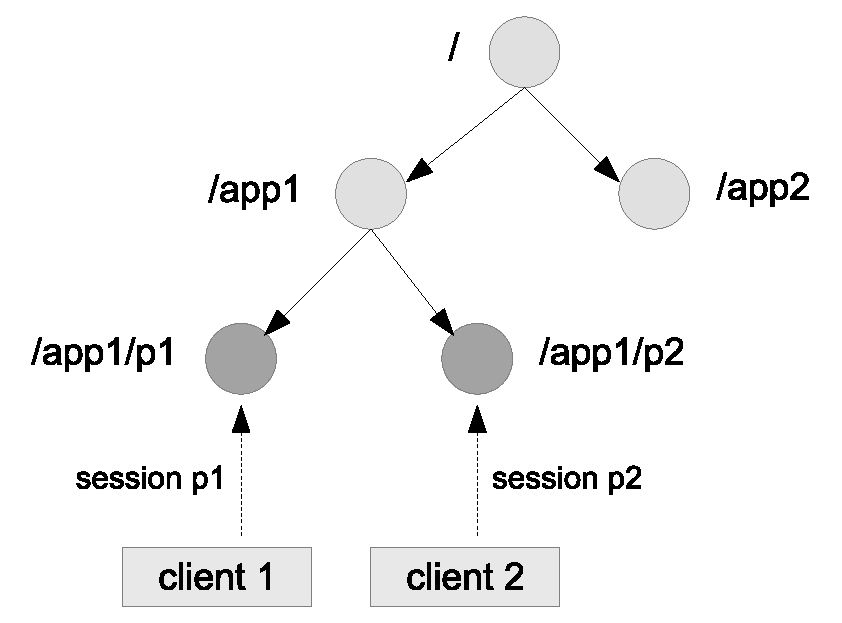
\includegraphics [width=0.5\textwidth]{images/zookeeper_tree}
  \caption{ZooKeeper tree sructure}
  \label{fig:zookeeper_tree}
\end{figure}

ZooKeeper is designed for small data warehousing, such as configuration, status and location information.
One node is usually not bigger than one kilobyte.
Therefore it stores data tree image in memory, keeping in a persistent store only transaction logs and snapshots.
In-memory storage limits the size of the database of ZooKeeper.
However, it gives advantages of low latency and high performance. 

The key feature of ZooKeeper is that it uses First In, First Out (FIFO) method for processing the messages.
It means that all commands are performed in the order they are received.
Thus, ZooKeeper maintains the total ordering.
The order is specified by a unique ZooKeeper Transaction id, that is assigned to each update.
 
ZooKeeper supports idempotent operations.
If a node should be updated, the system makes a note about the update and keeps an old and a new version of this node.
This allows client to receive the same message several times, being aware of when it can be applied.
Therefore all the write operations are performed sequentially in one thread and only on the master node.
On the contrary, read requests do not necessarily need the master node, they can be handled by a node's replica.

The client also supports the total ordering of the messages.
Hence if the client sends a write request and then a read request, the write operation is performed first.
Even if usually read operation does not need a lock, ZooKeeper strictly follows the order.
It allows to implement predictable asynchronous systems that work with ZooKeeper.

A client can watch a node.
If it sets a watch, it gets notified when the node is changed.
When the node sends this notification, it removes the watch.
In the case of connection problems between the client and the ZooKeeper server, the client receives a local notification.

ZooKeeper guarantees reliability using replication.
Its database is replicated to several nodes, one of them is a \textit{Leader} and the others are \textit{Followers}.
\textit{ZooKeeper Atomic Broadcast} (Zab) algorithm is used for managing the communication between the leader and the followers.
It synchronizes the replicas, broadcasts updates and recovers the valid state in the case of nodes crash.

Zab includes four phases: (1) Leader election, (2) Discovery, (3) Synchronization and (4) Broadcast.

1. On the first stage ZooKeeper uses any election algorithm to choose a leader.
After termination every node stores its vote locally in volatile memory.
When a node \textit{n} votes for a node \textit{n'}, \textit{n'} becomes a \textit{prospective leader} for \textit{n}.

2. On the second stage the nodes inform the prospective leader about the most recent transactions they accepted.
Thus the prospective leader knows the latest sequence af accepted transactions and can establish a new epoch.
From thit moment the previous leaders cannot perform any commits.
In the case of connection problems between a follower and a leader, the follower goes back to the stage (1) of this algorithm.

3. The leader is aware of the latests transactions history and during this stage synchronizes this information with its replicas.
This phase is also called voting phase, because it receives the votes from the nodes.
The leader performes a commit only if it receives acknowledgements from two of three followers.
At this moment the leader changes its state from \textit{prospective} to \textit{established}.

4. The nodes persist in this stage until a crash.
Every write request from a ZooKeeper client is broadcasted among the nodes.
New followers can join, receiving the transaction history from the leader.
The leader and its followers use periodic heartbeat messages for early failure detection.
If any of the nodes does nor receive a heartbeat message within a timeout, it shifts its state to \textit{election} and goes back to the first stage.

It can happened that one of the followers still has an outdated information when it receives the read request.
To avoid this problem, it is possible to make a force synchronisation with the master.
It is called the \textit{slow read}.
Evidently, if all the clients use the slow read the system looses the advantage of scaling.
Without force synchronisation ZooKeeper system scales for reads nicely. 
However, in this case the client that reads from a replica can obtain the outdated information.
\chapter{The Menthal Speed Layer}
\label{chap:menthal_backend_architecture}

This chapter serves as a delimiter between two global parts of our work.
The first part, that contains the previous chapters, is an observation part.
It presents the current problem of the Menthal project and the solutions offered by the world of the Big Data technologies.
It describes how global companies like Google or Facebook handle Big Data, what software tools and concepts are available in this sphere. 
Starting from this chapter only the information about our own project is presented.
This chapter includes functional and non-functional requirements to our system, its design, aspects of implementation and observation of several use cases.

\section{Requirements Analysis [SP]}
To determine the Menthal functional and non-functional requirements, first of all we need to formulate its use cases.
Figure~\ref{fig:menthal_use_case_diagram} represents the Use case diagram of Menthal project.
The system consists of two main parts, the client and the server.
This already gives a separation among its users.
On the one side, a user interact with a client application.
Menthal tracks the user behavior and provides a feedback, that is based on the gathered data analysis.
On the other side, system administrators and scientists interact with a server part.
Scientists carry on researches, analysing the obtained information.
A system administrator maintains the system, controls event processing and performes new analysis required by scientists.

\begin{figure}[h]
  \centering
  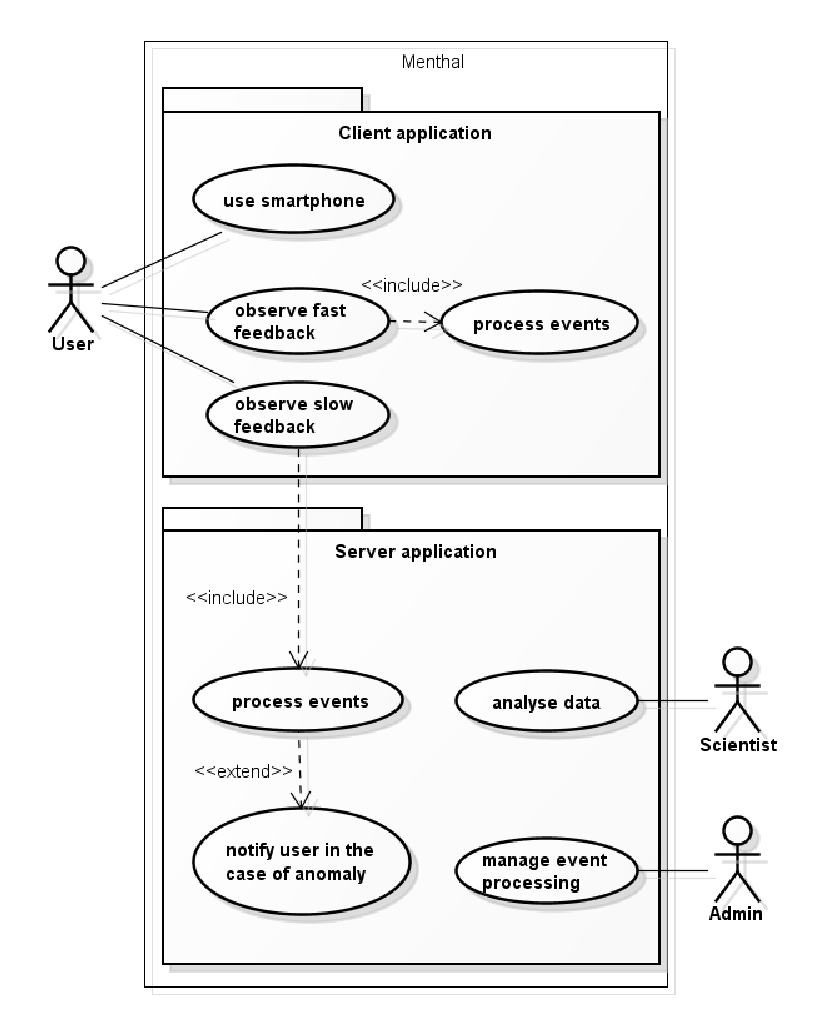
\includegraphics [width=0.9\textwidth]{images/menthal_use_case_diagram}
  \caption{Menthal Use case diagram}
  \label{fig:menthal_use_case_diagram}
\end{figure}


\subsection{Functional Requirements}

% to analyze speed layer architecture
The scope of our work is a part of Lambda Architecture named a Speed Layer.
% it consists o three components
% three parts for: receivivg data, ..
It requires to implement three main parts: data receiving part, real-time data processing and the store of the results of computations.
The data receiving part does not need to provide any feedback except the acknoledgement that the data was succeessfully received.
Thus on this end of the system we do not need any special API.
On the contrary, the results of computations can be used further by the other components of the Lambda architecture.
Therefore it can be useful to provide an API that allows to request the necessary information.

% ��������� ����� ��� speed layer, ���� �� ��� ��� ��� ��������?
% or give a big picture (how data goes)


\mnote{Event receiving}
The data receiving part collects the data that arrives from a message queue.
This data consists of various events that represent the actions a user performs on its smartphone. 
The responsibility of the data receiver is to deserialize incoming messages, identify the types of events and let the processing part to handle them.

\mnote{Aggregations}
The processing part of the Speed Layer performs various aggregations on the incoming data.
The distinctive feature of the Speed Layer is that it works only with limited amount of data, processing only the recent events.
Hence it can calculate aggregations and perform analisys in real time.
The created aggregations have different granularities and characterize the different aspects of user-smartphone interaction.

\mnote{Anomaly detection}
As the events are analyzed in real time, it gives an advantage of detecting various anomalies in incoming data.
We should use an appropriate anomaly detection algorithm that can be applied for the given data.
The system should detect the strange behavior in proper time and immediately notify a user if needed.

\mnote{Results storage}
The results of aggregations are stored while the Batch layer of the Lambda architecture performs its calculations.
During this time they should be available for queries.
Our system should provide an API for these purposes.
When the results of aggreagtions are collected from the Speed Layer and merged with the results from the Batch Layer, they can be deleted from a storage.
 
\subsection{Non-functional Requirements}

\mnote{Dependency on other components}
The Speed Layer as a part of the Lambda Architecture in particular and the Menthal project in general, needs to be designed taking into account its dependency on other system components
On the one hand, it should follow the principle of modularity, i.e. be self-contained.
Thus, when other parts of the system change, it should not influence the Speed Layer inner structure.
On the other hand, it should be flexible.
In the case of significant changes in the whole system, the adaptation process to the new environment should be fast and easy.

\mnote{Documentation}
All the available features of the Speed Layer should be well documented.
As other parts of the system are maintained by other developers, it is necessary to provide them with the most detailed and relevant description of the system.
It should be easy to obtain necessary information about the system capabilities, where to find the needed functional and how to use it.
Also it is important to provide a convenient mechanism for interpreting the occurring errors. 	    

\mnote{Extensibility}
The system must be easy extendable by additional functionalities.
From the technical side, the Speed Layer consists of a number of cooperating technologies.
These third-party technologies actively develop, the versions of software upgrade.
Therefore our system should allow easy upgrading of its components without a threat of failure.
From the application side, the Menthal project has a great development potential.
New features are constantly added, the functionality is expanded.

\mnote{Security}
Our system needs to meet high security requirement.
Menthal works with user data and stores personal information of real people.
Therefore it is important to protect the stored information from unauthorized access.
The source of information is a smartphone, that transfers collected data to the server.
The data store on the phone and the communication channel should be protected properly.
However, the security problems of these parts of the system are beyond the scope of our work.
We should provide a secure storage system for the results of aggregations, made on the received user data.
Furthermore, only authorized parties can get an access to these results.

\mnote{Performance}
As the Speed Layer should provide the results of data processing in real time, it puts one more requirement on our system.
It should have good performance characteristics.
In our case the costs of processing cores, physical memory and therefore the number of machines needed to perform calculations is less significant than the system performance.
It should work with the fixed and relatively small response time. 

\mnote{Availability and Reliability}
The system must be available and reliable.
The Speed Layer is the only component that has calculated aggregations on the latest data.
Moreover, for anomaly detection purposes it is important not to miss the significant changes in incoming data and react to them in a timely manner.
Therefore, the system should tend to be always available to provide the results of the performed aggregations.
Also it should constantly process the incoming data without failing to avoid the loss of the significant changes that are needed for anomaly detection. 

\mnote{Fault tolerance}
A real-time system should be fault tolerant.
In the case of Speed Layer it is especially relevant, because it consists of many cooperating components.
Even if several nodes in the cluster crash, it should not break the whole system and interrupt the calculation process.
For example, if the server receives the irrelevant event or the message is broken, it should notify about the problem adding an appropriate message into the log file.
However, this incident in no circumstances can be the reason of the whole system crash.
Furthermore, the Speed Layer should have small recovery time in the case of failure. 

\mnote{Efficiency}
We use commodity machines to construct the cluster where the server part of Menthal runs.
Thus it is necessary for our system to be highly efficient.
It should use the given resources in a proper way, allowing other components of the server part run on the same cluster in the full extend.

\mnote{Scalability}
The system load in the Menthal project depends on two main factors.
First, the increasing number of users auguments the load.
This can happen with the growth of popularity of the Menthal application.
Second, the variety of gathered information about user can be extended.
Hence our system should meet the requirement of scalability.
It should be possible to easily add new nodes in the cluster in the case of increasing load.  

\mnote{Codability}
During the development we should take into account the codability of the given system.
The amount of the required man-hours to finish the project is an important indicator of a well thought-out system.
In our case there are several different ways to implement the Speed Layer.
Having the same result, some of them require more effort from a programmer than the others.
It is necessary to choose a right strategy to create a working system.

\mnote{Maintainability}
Our goal is to build a working Speed Layer, however later other people will maintain it and perform the further development.
Thus the maintainability of our system is a significant requirement.
It should be easily configurable.
It need to provide a convenient mechanism to perform the tracking of the running tasks, e.g. using log files.
Finally, our system should have necessary tools for testing its functionality.

These requirements vary in their origins, goals and realisation complexity.
For example, scalability and extensibility are the essential properties of any distributed system.
The real-time processing requires availability, reliability and fault tolerance.
The maintainability and good documentation are easily reachable, they only need a proper approach for software development process.
On the contrary, such requirements as high security and good performance can be hard to implement.
In our work we tried to meet most of these requierements.  


\section{Design of the system [VI]}

Architecture of our system essentially repeats common design of the Speed layer, described in the Section~\ref{sec:speed_layer}.
The system consists of three main components: data source, data processing, and data storage.
Figure~\ref{fig:SpeedLayerArchitecture} depicts the general structure of the system.
Data source component is essentially beyond the inner architecture of the system.
Nevertheless, we consider it as a part, because it provides data, and we use specific libraries and classes to work with it.
Data processing component, implemented using Storm, is the core of the system.
It executes computations, and stores results to the data storage for further use.
Data storage component, that uses Redis key-value store, is a temporal database for maintaining real-time views.
Those views are then accessed by the Serving layer for query answering.

\begin{figure}[h]
  \centering
  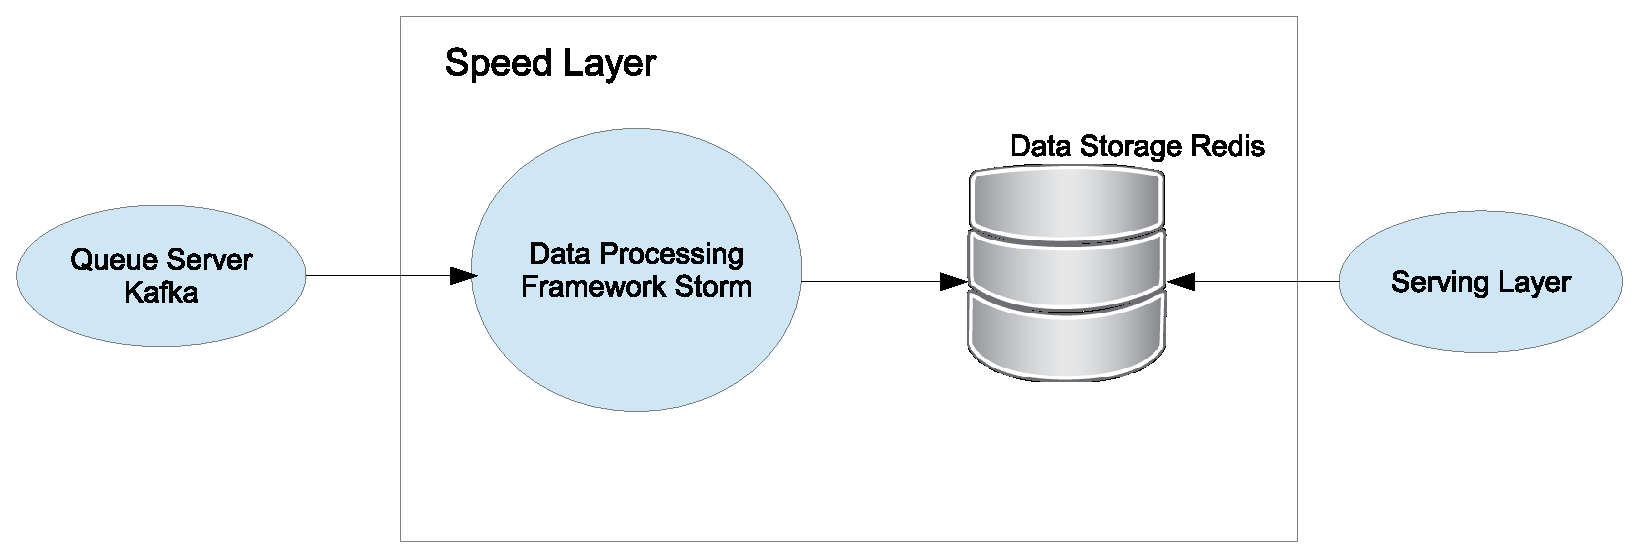
\includegraphics [width=1.0\textwidth]{images/SpeedLayerArchitecture}
  \caption{General structure of our system.}
  \label{fig:SpeedLayerArchitecture}
\end{figure}

\subsection{Data source}

The source of data, that is being processed, is the Kafka queue server \ref{subs:kafka}.
In its turn, it receives data from the outer sources, specifically from smartphones.
There are so far tens of thousends of smartphones, that use Menthal application and send data to the server.
Their number can grow arbitrarily, what requires in essence to have such a complex distributed server.
Smartphones send data to the server in small batches, that contain about fifty events, that happened since the last sending.
Kafka queue server stores this data temporarily, and tries to send it to all consumers, until they acknowledge delivery.
Our system is one of the consumers, and when it receives data, it starts processing. 

For each event type Kafka queue server maintains a dedicated topic.
It is possible then to subscribe for receiving of those events, that are needed for processing.
Events are sent as Avro objects \ref{subs:avro}, and contain meaningful information about what user does on the phone.
In our case we consider event types presented in the Table~\ref{table:event_types}.

\begin{table}[h]
\begin{tabular}{ | l | p{10cm} |}
    \hline
    AppInstall & Contains user id, app name and timestamp. Generated when the user installed a new application. \\ \hline
    AppSession & Contains user id, app name, timestamp and duration. Generated when the user has finished a session of using application. \\ \hline
    CallMissed & Contains user id, timestamp and contact hash. Generated when the user missed a call. Contact hash specifies a contact, that called. \\ \hline
    CallOutgoing & Contains user id, timestamp, contact hash and duration. Generated when the user finished an outgoing call. Contact hash specifies a contact, to that the call was addressed. \\ \hline
    CallReceived & Contains user id, timestamp, contact hash and duration. Generated when the user finished an incoming call. Contact hash specifies a contact, that called. \\ \hline
    DreamingStarted & Contains user id and timestamp. Generated when the phone gone to the dreaming mode. \\ \hline
    DreamingStopped & Contains user id and timestamp. Generated when the phone woke up from the dreaming mode. \\ \hline
    PhoneShutdown & Contains user id and timestamp. Generated when the phone goes off. \\ \hline
    ScreenOff & Contains user id and timestamp. Generated when the phone's screen goes off. \\ \hline
    ScreenOn & Contains user id and timestamp. Generated when the phone's screen goes on. \\ \hline
    ScreenUnlock & Contains user id and timestamp. Generated when the phone's screen is unlocked. \\ \hline
    SmsReceived & Contains user id,  timestamp, contact hash and message length. Generated when an sms is received. Contact hash specifies the contact, from that sms has come. \\ \hline
    SmsSent & Contains user id,  timestamp, contact hash and message length. Generated when an sms is sent. Contact hash specifies the contact, to that sms was sent. \\ \hline
    WindowStateChanged & Contains user id, timestamp, app name and window title. Generated when the new window becomes active. \\
    \hline
\end{tabular}
\caption{Event types and their descriptions}
\label{table:event_types}
\end{table}

\mnote{Kafka spout}
To obtain events from the Kafka queue server, we use \textit{Kafka spouts}.
Kafka spout is the class in the Storm's external class library, that allows to use Kafka queue server as a source of data for processing in the topology.
It listens for messages coming from Kafka in a particular topic.
Each such spout works in a distributed fashion, so that no matter how many events of a particular type will come, we can overcome this simply adding more machines to the cluster.

\subsection{Data processing}

The data processing framework Storm \ref{subs:storm} is the main component of the system.
It receives messages from Kafka queue server, and performs different computations on that data.
Its purpose is to provide different aggregatons on data coming from smartphones.
These aggregations are then stored in the storage system, and can be accessed by the Speed layer for answering queries.

The core of Storm framework is topology.
Topology describes the flow of computational logic.
It contains spouts and bolts, that represent data sources and data processing nodes, respectively.
We have already discussed Kafka spout, that we use for receiving data from the Kafka queue server.

Our topology has simple structure, but nevertheless has many nodes inside.
First of all, for each event type there is dedicated Kafka spout, that receives data from the Kafka queue server.
For that sake each Kafka spout is subscribed for a specific Kafka topic, corresponding to that event type.
When new message comes from the Kafka queue server, Storm runs particular spout on any available cluster node.

There is a dedicated bolt for each event type in our topology.
For each bolt we create a dedicated class, that performs particular processing, depending on what event type is it.
We use Storm's class \lstinline{BaseRichBolt} as a base class for all our bolts.
Our abstract class \lstinline{EventProcessingBolt}, that extends \lstinline{BaseRichBolt}, provides base functionality for all other bolts.
Every particular bolt class implements abstract method \lstinline{processEvent}, given in the class \lstinline{EventProcessingBolt}.
Such class hierarchy allows to add new event types for processing easily.
We just need to create new class, that inherits from \lstinline{EventProcessingBolt} and implements method \lstinline{processEvent}.

Class \lstinline{EventProcessingBolt} has a method \lstinline{getEventProcessingBoltByEventName}, that creates new bolt class by its name.
To achieve such functionality, class \lstinline{EventProcessingBolt} has protected field \lstinline{schemaName}.
It must be initialized in each derived class with the name of this particular event type.
This is useful again for the sake of extensibility, because it let's to leave code of topology initialization the same, no matter how many new event types we add for processing.
The main method of the \lstinline{EventProcessingBolt}, namely \lstinline{execute}, is presented on the Listing~\ref{listing:EventProcessingBolt_execute}.

\begin{lstlisting}[float=h, caption=The main method of the EventProcessingBolt., label=listing:EventProcessingBolt_execute, language=Java]
public void execute(Tuple tuple) {
  try {
    Schema schema = new Schema.Parser().parse(new File(schemaName + ".avsc"));
    DatumReader<GenericRecord> datumReader = new GenericDatumReader<GenericRecord>(schema);
    InputStream in = new ByteArrayInputStream((byte[])tuple.getValue(0));
    GenericRecord record = datumReader.read(null, DecoderFactory.get().jsonDecoder(schema, in));
    processEvent(record);
    _collector.emit(new Values(record));
  } catch (Exception e) {
    System.out.println("Exception raised!");
    System.out.println(e.getMessage());
  }
}
\end{lstlisting}

In the Line 3 we parse the schema of that particular event type.
Then in Lines 4-6 we parse input event to a \lstinline{GenericRecord} object using that schema.
\lstinline{GenericRecord} is an Avro class for representation of Avro objects in memory.
In the Line 7 we call abstract method \lstinline{processEvent}, that executes particular processing depending on what exact bolt class is it.

\lstinline{EventProcessingBolt} holds a reference to an interface \lstinline{EventAggregator}.
This interface provides method for processing all of event types that we consider.
Listing~\ref{listing:EventAggregator} shows the snippet from the definition of that interface.
We implemented exact class \lstinline{RedisEventAggregator} that realizes this interface.
As it states in its name, it works with Redis data storage.

\begin{lstlisting}[float=h, caption=The partial listing of the interface EventAggregator., label=listing:EventAggregator, language=Java]
public interface EventAggregator {
  void processAppSession(long userId, long time, long duration, String appName);
  void processCallMissed(long userId, long time, String contactHash, long timestamp);
  void processScreenOn(long userId, long time);
  void processSmsSent(long userId, long time, String contactHash, int msgLength);
  void processWindowStateChanged(long userId, long time, String appName, String windowTitle);
  ...
}
\end{lstlisting}

To make an example, let us consider one particular bolt class - \lstinline{AppSessionBolt}.
Listing~\ref{listing:AppSessionBolt} presents it.
In the constructor we initialize \lstinline{schemaName} with the name of this event type.
It is useful for creation of bolts by name.
In the method \lstinline{processEvent} we print out given record, then retrieve data fields from it, and pass them to a specific method of the \lstinline{eventAggregator} object, called \lstinline{processAppSession}.

\begin{lstlisting}[float=h, caption=Implementation of AppSessionBolt class., label=listing:AppSessionBolt, language=Java]
public class AppSessionBolt extends EventProcessingBolt {
  public AppSessionBolt() {
    schemaName = "app_session";
  }

  @Override
  protected void processEvent(GenericRecord record) {
    System.out.println(schemaName + "-Bolt: " + record.toString());
    long userId = (long)record.get("userId");
    long time = (long)record.get("time");
    long duration = (long)record.get("duration");
    String appName = record.get("appName").toString();
    eventAggregator.processAppSession(userId,time,duration,appName);
  }
}
\end{lstlisting}

On the events coming from smartphones we do different aggregations.
They will be then taken by the Serving layer for answering queries.
There are three types of aggregation, that we maintain in the data storage: counter, duration, and lenght.
Counter collects the number of events of any particular type.
Duration accumulates the total duration of the continuing action on the smartphone.
Length contains the total length of sms or whatsapp messages, etc.
There is a different logic of how to compute them for these three types of aggregations. 
For each aggregation we store four cases for different time intervals: last hour, last day, last week, last month.
Specifically, for each aggregations consists of two value: timestamp of the start of the current hour/day/week/month, and aggregation value itself.
Each time we update aggregation, that requires to recompute its starting timestamp.

\subsection{Data storage}

Data storage Redis \ref{subs:redis} keeps all results of computations.
These results are different aggregations, specifically counters, that are stored in the complex data model.
Redis provides simple access to save and then get that data.
Counters, saved in the Redis data storage can be then used by the Speed layer to merge them with the results of batch computations.

Redis is a key-value store, what defines the approach of storing data.
Each aggregations that we save to Redis is a list of two values: timestamp and value.

To work with aggregations in Redis we have developed a concrete class \lstinline{RedisEventAggregator}, that implements an interface \lstinline{EventAggregator}.
It works with the object of the type \lstinline{RedisProxy}, that we discribe later on in this section.
Each method of the class \lstinline{RedisEventAggregator} receives arguments as for example: user id, timestamp, app name, etc.
We then combine these values to a proper key name, that is present in Redis (or must be created on the first update).
Listing~\ref{listing:processAppSession} shows an example of key creation and passing it to \lstinline{RedisProxy}.

\begin{lstlisting}[float=h, caption=Example of key creation for aggregation update., label=listing:processAppSession, language=Java]
public void processAppSession(long userId, long time, long duration, String appName) {
  String key = String.format("app:%s:%s", appName, "sessions");
  redisProxy.incrementCounters(key, time);
  key = String.format("app:%s:%s", appName, "total_time");
  redisProxy.incrementDurations(key, time, duration);
  ...
\end{lstlisting}

We keep keys in Redis in the following way.
Each key is associated with the list, that has two elements.
The first one is the timestamp of the beginning of counting.
The second one is the value itself.
There are several examples of the keys in the Listing~\ref{listing:keysInRedis}.

\begin{lstlisting}[float=h, caption=Examples of the keys in Redis., label=listing:keysInRedis]
user:$user_id:$phone_hash:incoming_msg_count:count:hourly
user:$user_id:$phone_hash:incoming_msg_count:count:daily
user:$user_id:$phone_hash:incoming_msg_count:count:weekly
user:$user_id:$phone_hash:incoming_msg_count:count:monthly
user:$user_id:$phone_hash:outgoing_call_duration:duration:hourly
user:$user_id:$phone_hash:outgoing_call_duration:duration:daily
user:$user_id:$phone_hash:outgoing_call_duration:duration:weekly
user:$user_id:$phone_hash:outgoing_call_duration:duration:monthly
user:$user_id:$phone_hash:outgoing_msg_length:length:hourly
user:$user_id:$phone_hash:outgoing_msg_length:length:daily
user:$user_id:$phone_hash:outgoing_msg_length:length:weekly
user:$user_id:$phone_hash:outgoing_msg_length:length:monthly
\end{lstlisting}

To access Redis we use Jedis java library \cite{Jedis}.
It provides the the whole functionality, that Redis offers itself.
The class \lstinline{RedisProxy} contains all the communication with Redis.
It contains two fields, presentd on the Listing~\ref{listing:RedisProxyFields}.
They are the part of the Jedis library, and provide exact access to the Redis database.

\begin{lstlisting}[float=h, caption=Two main fields of the class RedisProxy., label=listing:RedisProxyFields, language=Java]
private final Jedis jedis;
private Pipeline pipeline;
\end{lstlisting}

\mnote{Pipeline}
We use \textit{pipelines} to communicate with Redis database.
Pipeline allows to combine several reqests to Redis into one batch, and send it altogether to the server through the network.
It reduces network congestion, and makes probability of race conditions on the server less.
\mnote{Transaction}
Inside of pipeline we use \textit{transaction} to tell Redis server, that we this set of commands must be executed as a one atomic command.
This is important to avoid race conditions, because many clients in the same time can try to access the same keys in the Redis database.
We demonstrate changing of the counter on the Listing~\ref{listing:incrementCounter}.

\begin{lstlisting}[float=h, caption=Example of updating counter aggregation in the Redis database., label=listing:incrementCounter, language=Java]
private void incrementCounter(DurationType durationType, CounterType counterType, String key, long time, long valueToIncrement) {
  key = String.format("%s:%s:%s", key, getCounterName(counterType), getDurationName(durationType));
  Boolean success = false;
  while (!success) {
    jedis.watch(key);
    List<String> value = jedis.lrange(key, 0, 1);
    pipeline = jedis.pipelined();
    pipeline.multi();
    Counter counter = new Counter(durationType, Long.parseLong(value.get(0)), Long.parseLong(value.get(1)));
    if (updateStartingTime(counter, time, 0))
      pipeline.lset(key, 0, Long.toString(counter.startTime));
    counter.value += valueToIncrement;
    pipeline.lset(key, 1, Long.toString(counter.value));
    success = (pipeline.exec() != null);
  }
  pipeline.sync();
}
\end{lstlisting}

We first generate in the Line 2 a proper key, that exactly exists in Redis, from a base key part.
Then we do do watching for values, that we want to retrieve and then change.
This is necessary to do, because this is the only way to protect the whole operation from race condition on the server side.
We get value of the counter in the Line 6.
Then in the Lines 7-8 we initialize pipeline and transaction.
In the Lines 9-12 we update retrieved counter in memory.
And in the Line 13 we set the new value of the counter into Redis server.
If in the time between watch and update of key's value it was accessed by other client, operation will fail, and we try to execute it again.

\section{Use Cases [SP]}
\label{sec:use_cases}

This section presents two examples of using the Speed layer architecture, described above.
The main purpose of the Speed layer is to process the incoming events.
In the context of the Menthal project we need to calculate various aggregations.
In addition, our project allows to perform anomaly detection analysis.
These features are described in more detail below.

\subsection{Aggregations}

In our project we use two types of aggregations: user-based and application-based.
Table~\ref{fig:user_based_aggregations} represents the table of user-based aggregations.
Each of these aggregations is calculated with different granularities: hourly, daily, weekly and monthly.

\begin{table}
  \centering
  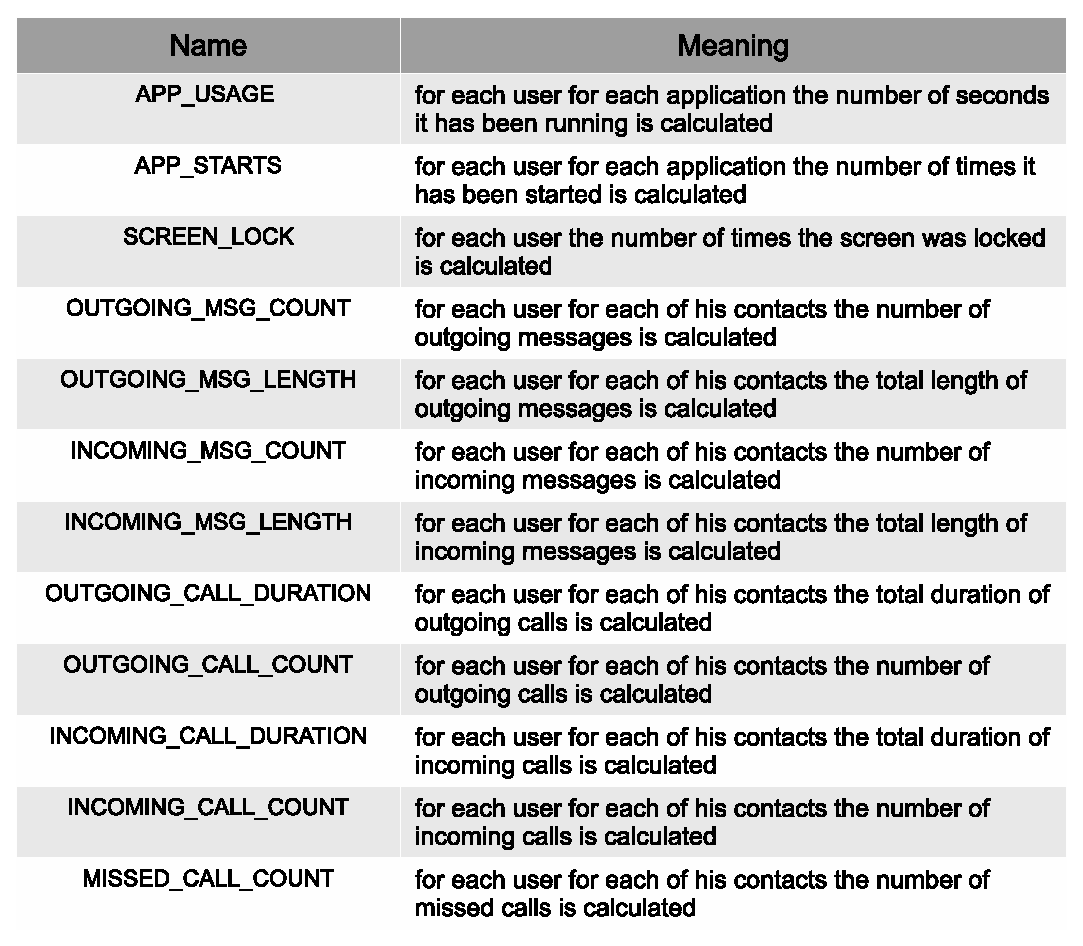
\includegraphics [width=1.0\textwidth]{images/user_based_aggregations}
  \caption{User-based aggregations}
  \label{fig:user_based_aggregations}
\end{table}

The aggregations presented in the table are made for each user separately.
However, all these aggregations except SCREEN\_LOCK are also implemented as a sum and average for all users. 
Another group of aggregations is global summaries for different applications.
We calculate for each application the number of unique users, the number of sessions and total time spent. 

The implementation of aggregations in our case is based on Redis.
There is an interface \textit{EventAggregator} that actually allows to use any other data storages.
However, in our work we concentrate on Redis implementation of this interface.
It perfectly fits our needs for fast access and this storage is easy to use and does not need a lot of programming effort.

\subsection{Anomaly Detection}

People download various applications for their smartphones and do not pay much attention to the questions of security.
There is a risk that applications from unofficial stores contain the malicious software.
Moreover, the software from an official store can turn out to be infected.
The main problem is that usually users do not read what personal information the application requests an access to.
And even if they read it, they do not have a choice to give the permissions or not.
Without giving the required access rights, a user cannot install this application on the smartphone.
   
The malicious software on smartphones behaves in different ways.
It can try to spread and infect all the contacts in a user's contact list.
For instance, a virus can send an sms, that contains its copy.
The virus can download and install another malicious software on the user's smartphone.
To apply some changes that the virus has performed in the system, it can restart the device.
Sometimes the malicious software can even make calls to specific numbers, so the user is charged for them.

\mnote{anomaly type}
As it was mentioned in section \ref{sec:anomaly_detection_algorithms}, there are a lot of ways to detect anomaly in incoming data.
Let us first decide what kind of anomaly we are dealing with.
Usually users do not have a strict pattern of interacting with their smartphones.
The sequence of performed actions changes from time to time.
One day a user can start with a phone call, another day by sending several messages.
This means that our anomaly is not \textit{collective}.
We consider a data instance independently from neighboring instances, therefore the anomaly type is not \textit{contextual}.
Thus we can conclude that we are dealing with the \textit{point} anomaly.

\mnote{anomaly detection approach}
Next step is to decide what approach to use for point anomaly detection.
The percentage of infected smartphones among the Menthal users is low.
It happens because the Android platform has good protection mechanisms and the official application stores are regularly tested for viruses.
Therefore we have a lot of \textit{normal} data and it is hard to get \textit{abnormal} examples (data from infected phones).
In this situation we cannot use supervised learning, so we have chosen an unsupervised approach.

\mnote{One-class SVM}
There are several anomaly detection techniques that implement an unsupervised approach.
We decided to use one-class support vector machines (SVM) technique, because it perfectly fits our demands.
First, it needs only 'normal' data instances for learning.
Also it can work with high-dimension data, i.e. when a feature vector consists of more than two features (we need four in our case).
Moreover, there is an existing java library called libsvm \cite{libsvm} that among other techniques implements one-class SVM.

Follow the assumed malicious software behavior, we try to detect the suspicious behavior of the smartphone.
For this purpose we analyze four events that are received from the clients: \textit{sms\_sent}, \textit{app\_install}, \textit{phone\_shutdown} and \textit{call\_outgoing}.
For simplicity we only count the number of these events.
However there is a possibility to make more thoughtful research, using the values that these events contain.
For example, traffic data, namely the number of transferred bytes, can be used for analysis.
To have a basis for comparing the amount of events, we use a time window.
In other words, for each type of event we calculate the number of times it occurs in a specified time interval (one hour by default).
Roughly speaking, we can take the number of times the event occurs in a normal state, than calculate this number for an unknown state and make a conclusion whether it is normal or abnormal.

To use One-class SVM algorithm we need to create a training data set.
When the training set is ready we run \textit{svm\_train} method to create a model.
Then we use \textit{svm\_save\_model} method to safe the trained model, so it can be used later for anomaly detection.

\mnote{flow of events}
The Speed Layer has the following architecture to allow anomaly detection of incoming data.
Figure~\ref{fig:anomaly_detection_data_flow} illustrates the data flow.

\begin{figure}[h]
  \centering
  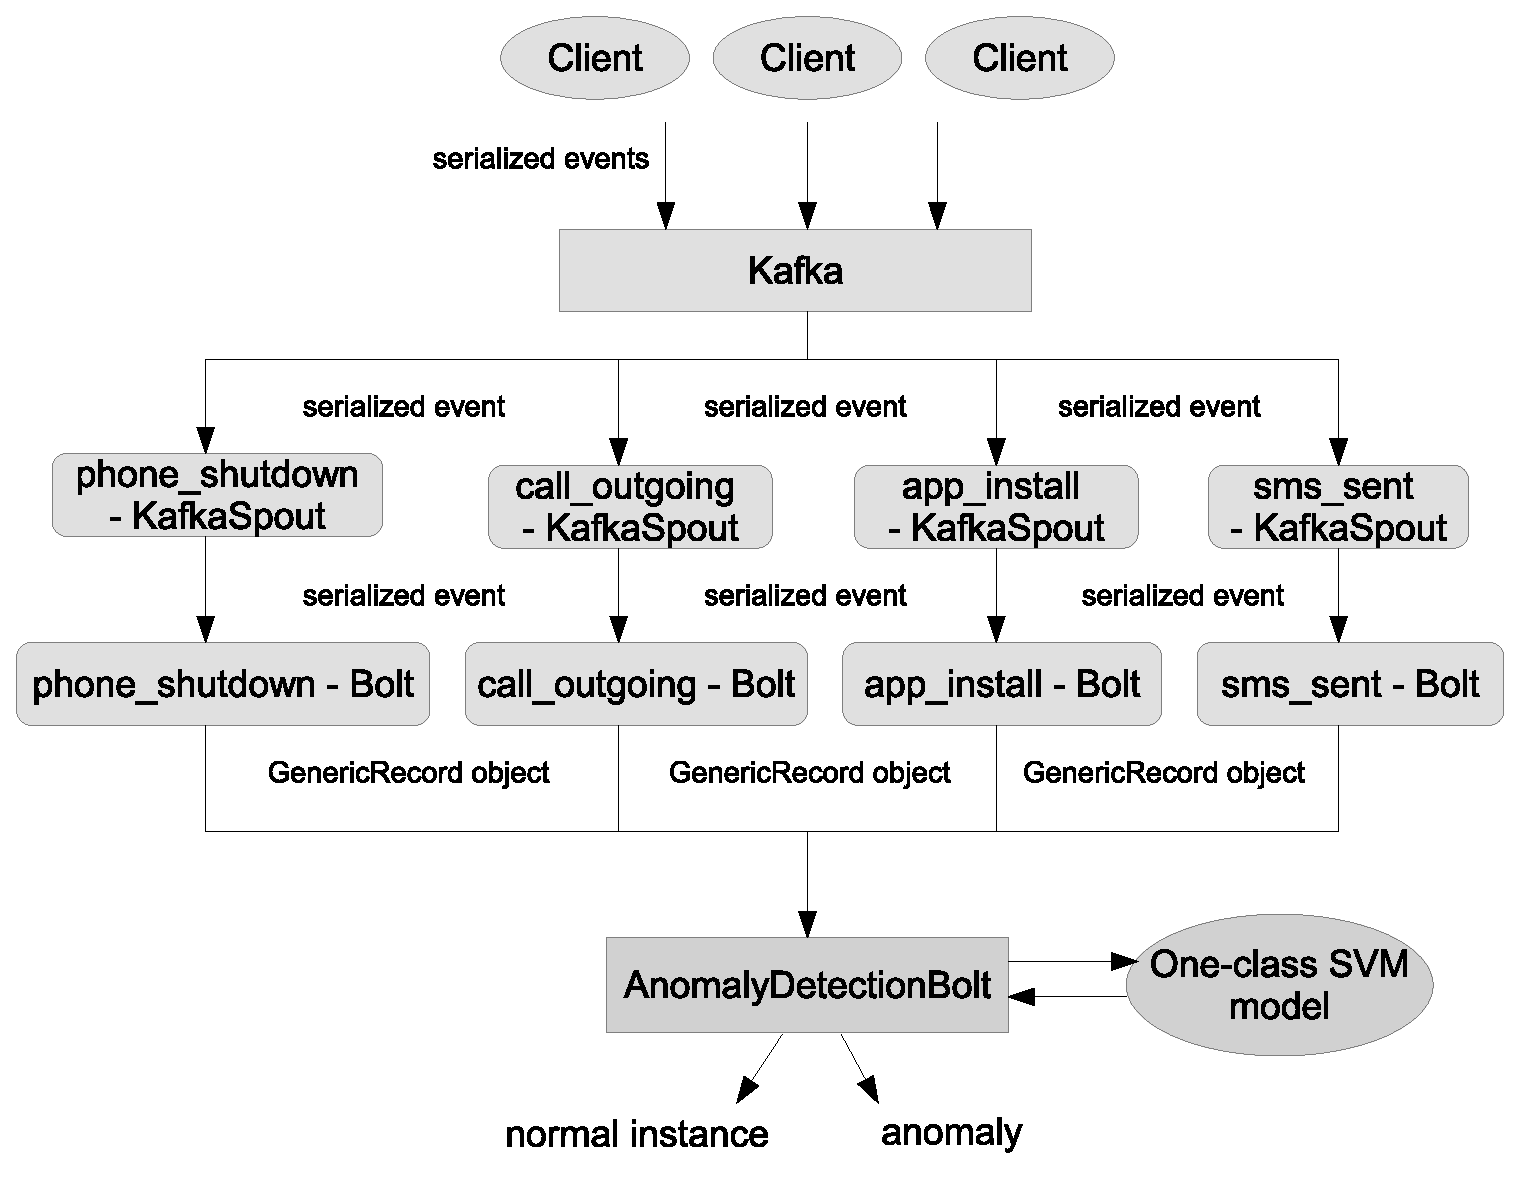
\includegraphics [width=1.0\textwidth]{images/anomaly_detection_data_flow}
  \caption{Anomaly detection: data flow}
  \label{fig:anomaly_detection_data_flow}
\end{figure}

For each Kafka topic a separate KafkaSpout receives messages.
One message contains the description of a particular event that happened on the client side (e.g. sms\_sent).
For each event type a separate bolt receives data from a corresponding KafkaSpout.
Then the bolt deserializes the received message, creating a \textit{GenericRecord} that represents the event.
For the events that are interesting for anomaly detection, there is an additional step.
Bolts, that receive data of type \textit{sms\_sent}, \textit{app\_install}, \textit{phone\_shutdown} and \textit{call\_outgoing}, emit the created GenericRecords to an \textit{AnomalyDetectionBolt}.

\mnote{Anomaly Detection bolt}
The main function of AnomalyDetectionBolt is to form data instances from incoming events.
As our version of Speed layer uses Redis as a data store, AnomalyDetectionBolt also uses it to accumulate events.
When a new event is received, AnomalyDetectionBolt extracts a type of event, a user id, and time when this event occurred.
Using the user id, the bolt requests the value of \textit{lastCheckTime} that is stored in Redis.
The \textit{lastCheckTime} value is compared with the time, extracted from the received event.
If the time delta is bigger than a specified threshold, the new check for anomaly is performed.
The frequency of anomaly checks is regulated by an ANOMALY\_CHECK\_INTERVAL parameter.
This mechanism sets only one-side bound, so the check is performed not more than every half an hour by default.
However, if the bolt rare receives events from a particular user, the check for anomaly is run with the same low frequency. 

AnomalyDetectionBolt uses a sliding window to accumulate events.
The size of the window is regulated by a TTL parameter.
TTL specifies how long the event is stored in Redis.
Each time the new check for anomaly is performed, the bolt first of all deletes all outdated events from the store.
This guarantees that the data instance that participates in anomaly detection contains events that are collected over a specified period.
For example, the size of the sliding window is one hour by default.
If we want to perform an anomaly detection analysis, we take the mentioned earlier four types of events and count how many times each of them has occurred during the last hour.
Using this numbers the bolt forms a data instance.  
Then it checks whether the instance is an anomaly or not using the trained one-class SVM model.

To get correct results it is essential to select the optimal parameters for One-class SVM.
Table~\ref{fig:svm_parameters} represents the parameters, their meaning and values that are optimal for our case.
The process of parameters selection includes a technique called \textit{cross-validation}.
Here the data set is divided into two parts - training set and testing set.
This helps to avoid the problem of model overfitting.  

\begin{table}[h]
  \centering
  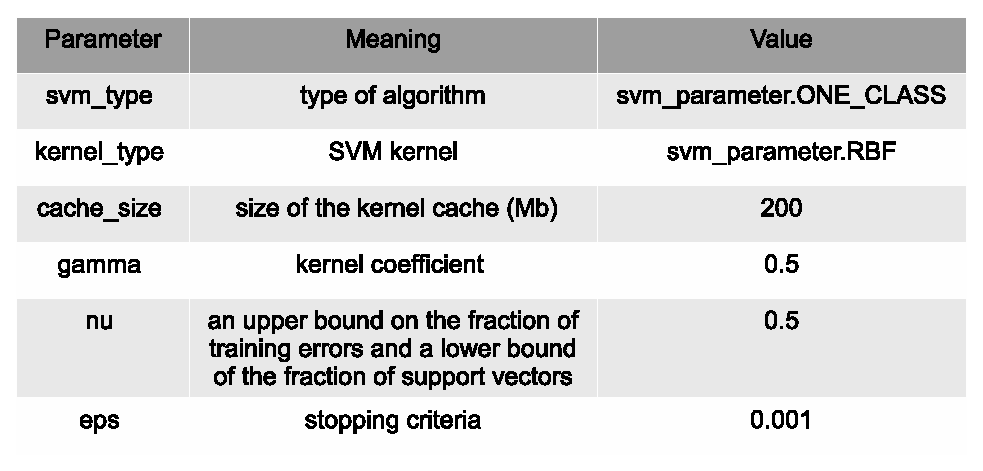
\includegraphics [width=0.9\textwidth]{images/svm_parameters}
  \caption{One-class SVM parameters}
  \label{fig:svm_parameters}
\end{table}







 	

 
 


%\section{Data flow}
%General schema (picture)
%3 pages

%\section{Algorithms}

%\section{Mapping to hardware}
%how many servers, characteristics, data transferring
%1 page

%\section{Aspects of implementation}
%programming languages, etc.

\chapter{Implementation}
\label{chap:implementation}

% rename chapter to Use cases

% first paragraph:
% architecture was described
% now we show how to use it
% two examples
% one subsection about aggregations
% one subsection about anomaly detection

Aggregations

In our project we use two types of aggregations: user-based and application-based.
Figure~\ref{fig:user_based_aggregations} represents the table of user-based aggregations.
Each of these aggregations is calculated with different granularities: hourly, daily, weekly and monthly.

\begin{figure}
  \centering
  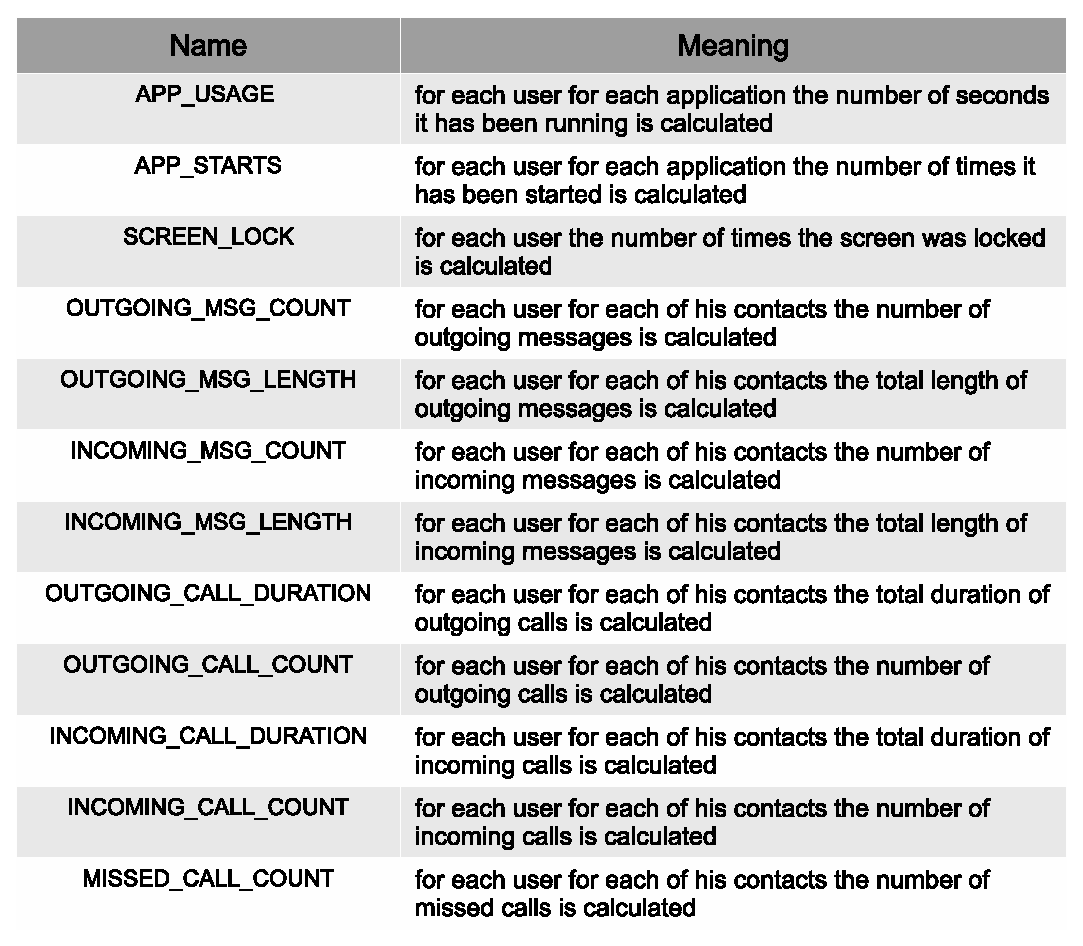
\includegraphics [width=1.0\textwidth]{images/user_based_aggregations}
  \caption{User-based aggregations}
  \label{fig:user_based_aggregations}
\end{figure}

The aggregations presented in the table are made for each user separately.
However, all these aggregations except SCREEN\_LOCK are also implemented as a sum and averadge for all users. 
Another group of aggregations is global summaries for different applications.
We calculate for each application the number of unique users, the number of sessions and total time spent. 

The implementation of aggregations in our case is based on Redis.
There is an interface \textit{EventAggregator} that actually allows to use any other data storages.
However, in our work we concentrate on Redis implementation of this interface.
It perfectly fits our needs for fast access and this storage is easy to use and does not need a lot of programming effort.


Anomaly Detection

People download various applications for their smartphones and do not pay much attention to the questions of security.
There is a risk that applications from unofficial stores contain the malicious software.
Moreover, the software from an official store can turn out to be infected.
The main problem is that usually users do not read what personal information the application requests an acces to.
And even if they read it, they do not have a choice to give the permissions or not.
Whithout giving the requred access rights, a user can not install this application on the smartphone.
   
The malicious software on smartphones behaves in different ways.
It can try to spread and infect all the contacts in a user's contact list.
For instance, a virus can send an sms, that contains its copy.
The virus can download and install another malicious software on the user's smartphone.
To apply some changes that the virus has performed in the system, it can restart the device.
Sometimes the malicious software can even make calls to specific numbers, so the user is charged for them.

\mnote{anomaly type}
As it was mentioned in Chapter , there are a lot of ways to detect anomaly in incoming data.
Let us first decide what kind of anomaly we are dealing with.
Ususally users do not have a strict pattern of interacting with their smartphones.
The sequence of performed actions changes from time to time.
One day a user can start with a phone call, another day by sending several messages.
This means that our anomaly is not \textit{collective}.
We consider a data instance independently from neighboring instances, therefore the anomaly type is not \textit{contextual}.
Thus we can conclude that we are dealing with the \textit{point} anomaly.

\mnote{anomaly detection approach}
Next step is to decide what approach to use for point anomaly detection.
The percentage of infected smartphones among the Menthal users is low.
It happens because the Android platform has good protection mechanisms and the official application stores are regularly tested for viruses.
Therefore we have a lot of \textit{normal} data and it is hard to get \textit{abnormal} examples (data from infected phones).
In this situation we can not use supervised learning, so we have chosen an unsupervised approach.

\mnote{One-class SVM}
There are several anomaly detection techniques that implement an unsupervised approach.
We decided to use one-class support vector machichenes (SVM) technique, because it perfectly fits our demands.
First, it needs only 'normal' data instances for learning.
Also it can work with high-dimension data, i.e. when a feature vector consists of more than two features (we need four in our case).
Moreover, there is an existing java library called libsvm [http://www.csie.ntu.edu.tw/~cjlin/libsvm/] that among other techniques implements one-class SVM.

Follow the assumed malicious software behavior, we try to detect the suspicious behavior of the smartphone.
For this purpose we analyze four events that are received from the clients: \textit{sms\_sent}, \textit{app\_install}, \textit{phone\_shutdown} and \textit{call\_outgoing}.
For simplicity we only count the number of these events.
However there is a possibility to make more thoroughtful research, using the values that these events contain.
For example, traffic data, namely the number of transferres bytes, can be used for analysis.
To have a basis for comparing the amount of events, we use a time window.
In other words, for each type of event we calculate the number of times it occures in a specified time interval (one hour by default).
Roughly speaking, we can take the number of times the event occures in a normal state, than calculate this number for an unknown state and make a conclusion whether it is normal or abnormal.

To use One-class SVM algorithm we need to create a training data set.
% TODO: write about training data

When the training set is ready we run \textit{svm\_train} method to create a model.
Then we use \textit{svm\_save\_model} method to safe the trained model, so it can be used later for anomaly detection.

\mnote{flow of events}
The Speed Layer has the following architecture to allow anomaly detection of incoming data.
Figure~\ref{fig:anomaly_detection_data_flow} illustrates the data flow.

\begin{figure}[h]
  \centering
  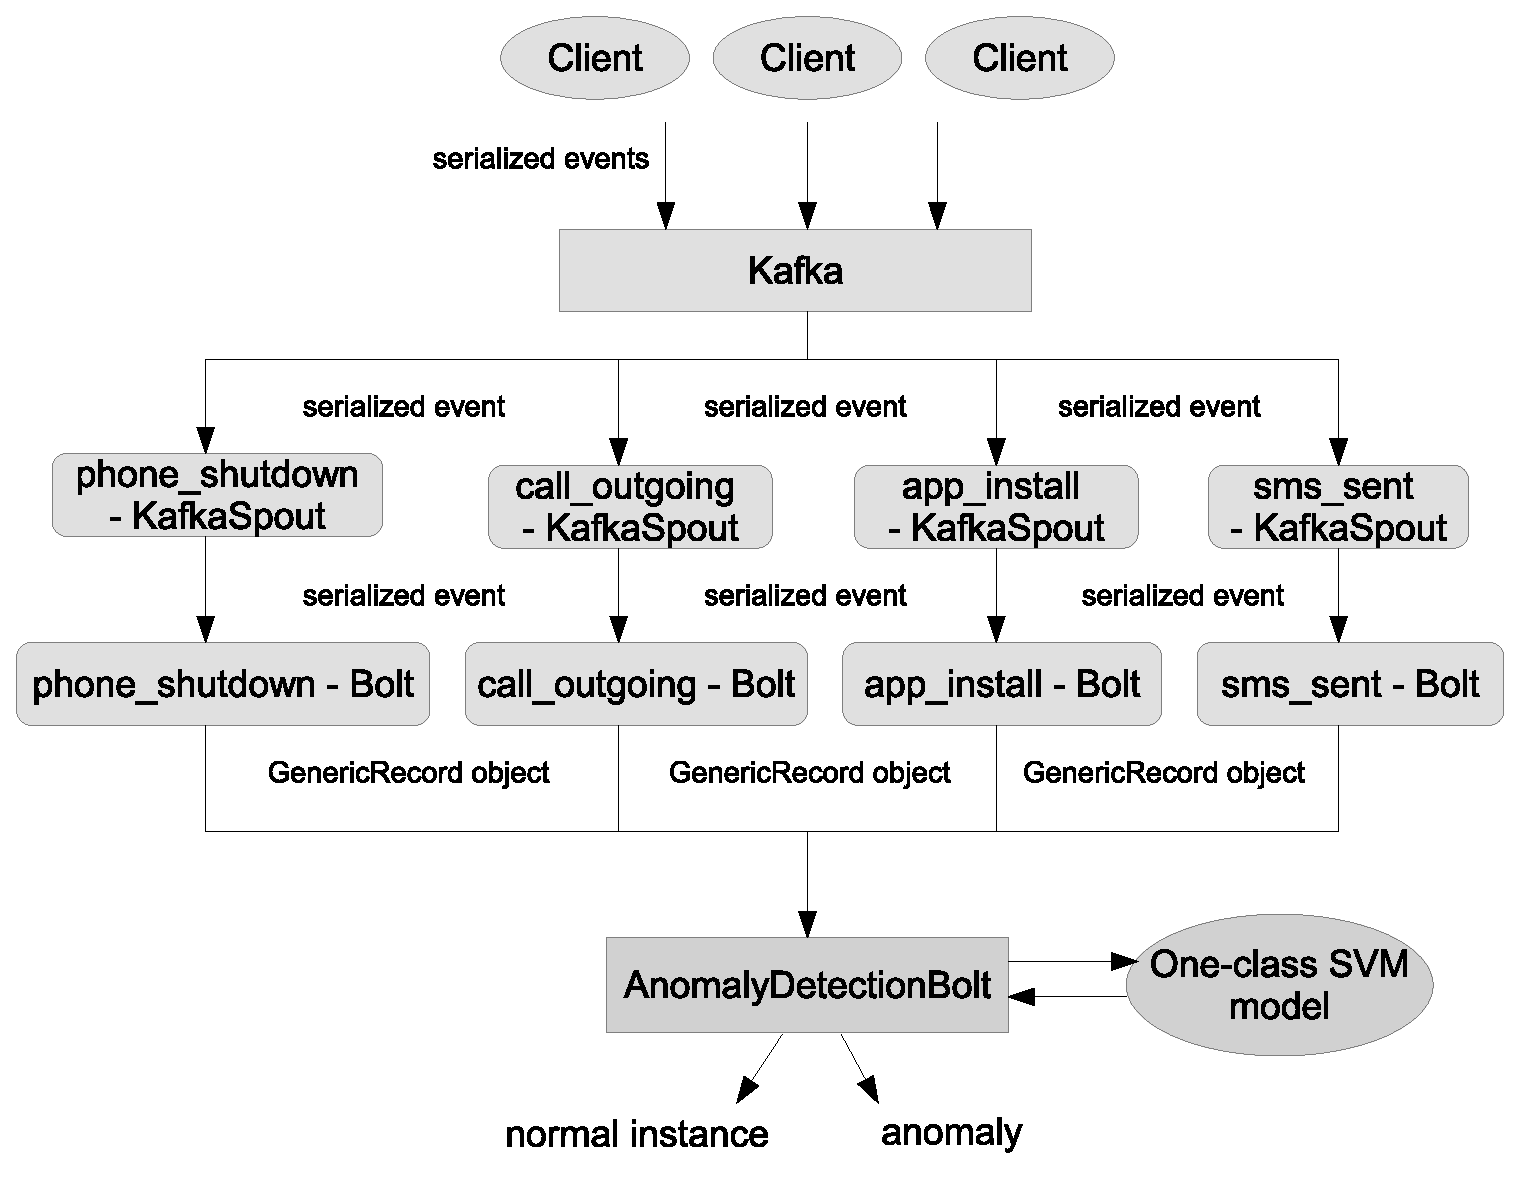
\includegraphics [width=1.0\textwidth]{images/anomaly_detection_data_flow}
  \caption{Anomaly detection: data flow}
  \label{fig:anomaly_detection_data_flow}
\end{figure}

For each Kafka topic a separate KafkaSpout receives messages.
One message contains the description of a particular event that happened on the client side (e.g. sms\_sent).
For each event type a separate bolt receives data from a corresponding KafkaSpout.
Then the bolt deserializes the received message, creating a \textit{GenericRecord} that represents the event.
For the events that are interesting for anomaly detection, there is an additional step.
Bolts, that receive data of type \textit{sms\_sent}, \textit{app\_install}, \textit{phone\_shutdown} and \textit{call\_outgoing}, emit the created GenericRecords to an \textit{AnomalyDetectionBolt}.

\mnote{Anomaly Detection bolt}
The main function of AnomalyDetectionBolt is to form data instances from incoming events.
As our version of Speed layer uses Redis as a data store, AnomalyDetectionBolt also uses it to accumulate events.
When a new event is received, AnomalyDetectionBolt extracts a type of event, a user id, and time when this event occured.
Using the user id, the bolt requests the value of \textit{lastCheckTime} that is stored in Redis.
The \textit{lastCheckTime} value is compared with the time, extracted from the received event.
If the time delta is bigger than a specified threshold, the new check for anomaly is performed.
The frequency of anomaly checks is regulated by an ANOMALY\_CHECK\_INTERVAL parameter.
This mechanism sets only one-side bound, so the check is performed not more than every half an hour by default.
However, if the bolt rare receives events from a particular user, the check for anomaly is run with the same low frequency. 

AnomalyDetectionBolt uses a sliding window to accumulate events.
The size of the window is regulated by a TTL parameter.
TTL specifies how long the event is stored in Redis.
Each time the new check for anomaly is performed, the bolt first of all deletes all outdated events from the store.
This guarantees that the data instance that participate in anomaly detection contains events that are collected over a specified period.
For example, the size of the sliding window is one hour by default.
If we want to perform an anomaly detection analysis, we take the mentioned earlier four types of events and count how many times each of them has occured during the last hour.
Using this numbers the bolt forms a data instance.  
Then it checks whether the instance is an anomaly or not using the trained one-class SVM model.

To get correct results it is essential to select the optimal parameters for One-class SVM.
Figure~\ref{fig:svm_parameters} represents the parameters, their meaning and values that are optimal for our case.
The process of parameters selection includes a technique called \textit{cross-validation}.
Here the data set is divided into two parts - training set and testing set.
This helps to avoid the problem of model overfitting.  

\begin{figure}[h]
  \centering
  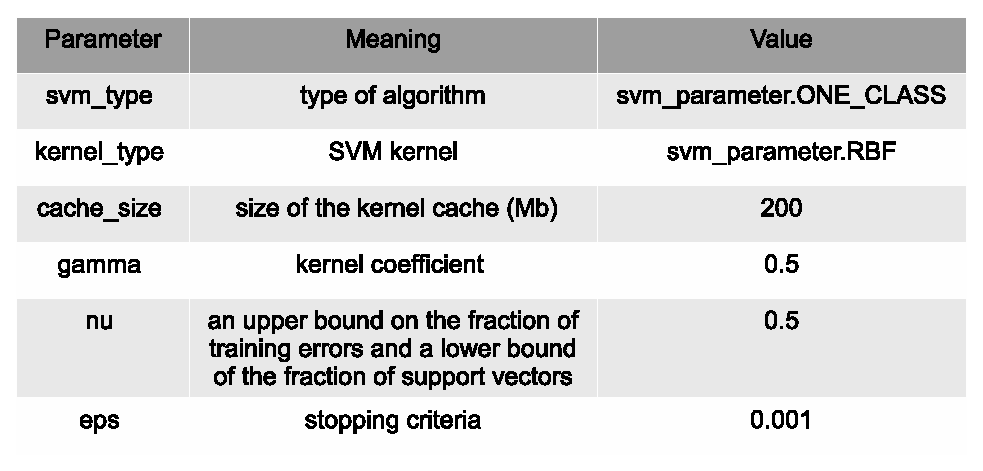
\includegraphics [width=0.9\textwidth]{images/svm_parameters}
  \caption{One-class SVM parameters}
  \label{fig:svm_parameters}
\end{figure}







 	

 
 

Part X Experiments

evaluation of possibilities of the system
\chapter{Summary}
\label{chap:summary}


%% Bibliographie
\backmatter
%\nocite{*}
\bibliography{bibliography/literature}

\appendix
\listoffigures
\listoftables
\lstlistoflistings

\end{document}
